\documentclass{beamer}

\usepackage{helvet}
\usepackage{bm}
\usepackage{graphicx}
\usepackage{breqn}
%\usepackage{enumerate}
\usepackage{wasysym}
\usepackage{amssymb}
\usepackage{hyperref}
\usepackage{color, colortbl}
\usepackage{enumitem}
\usepackage{ulem}
\usepackage{color}
\usepackage{tikz}
\usepackage{tabularx}
\usepackage{transparent}

\usetheme{progressbar}
\usefonttheme[onlymath]{serif}
\progressbaroptions{imagename=figures/lwa-antenna}

\newcommand{\tbf}{\textbf}
\renewcommand{\b}{\pmb}
\renewcommand{\d}{{\rm d}}
\newcommand{\rhat}{{\hat {\rm r}}}

\DeclareMathOperator{\Tr}{Tr}
\DeclareMathOperator{\argmin}{argmin}

\newcommand\Wider[2][3em]{%
    \makebox[\linewidth][c]{%
        \begin{minipage}{\dimexpr\textwidth+#1\relax}
            \raggedright#2
        \end{minipage}%
    }%
}

\definecolor{gray}{rgb}{.3,.3,.3}
\definecolor{red}{rgb}{1,0,0}
\definecolor{green}{rgb}{0,1,0}
\definecolor{blue}{rgb}{0,0,1}

\begin{document}
\title[Searching for the Cosmic Dawn]{
    Searching for the Cosmic Dawn with the\\
    Hyperfine Structure Transition of Hydrogen
}
\author{Michael Eastwood}
\date{September 3, 2018} 

{
    \usebackgroundtemplate{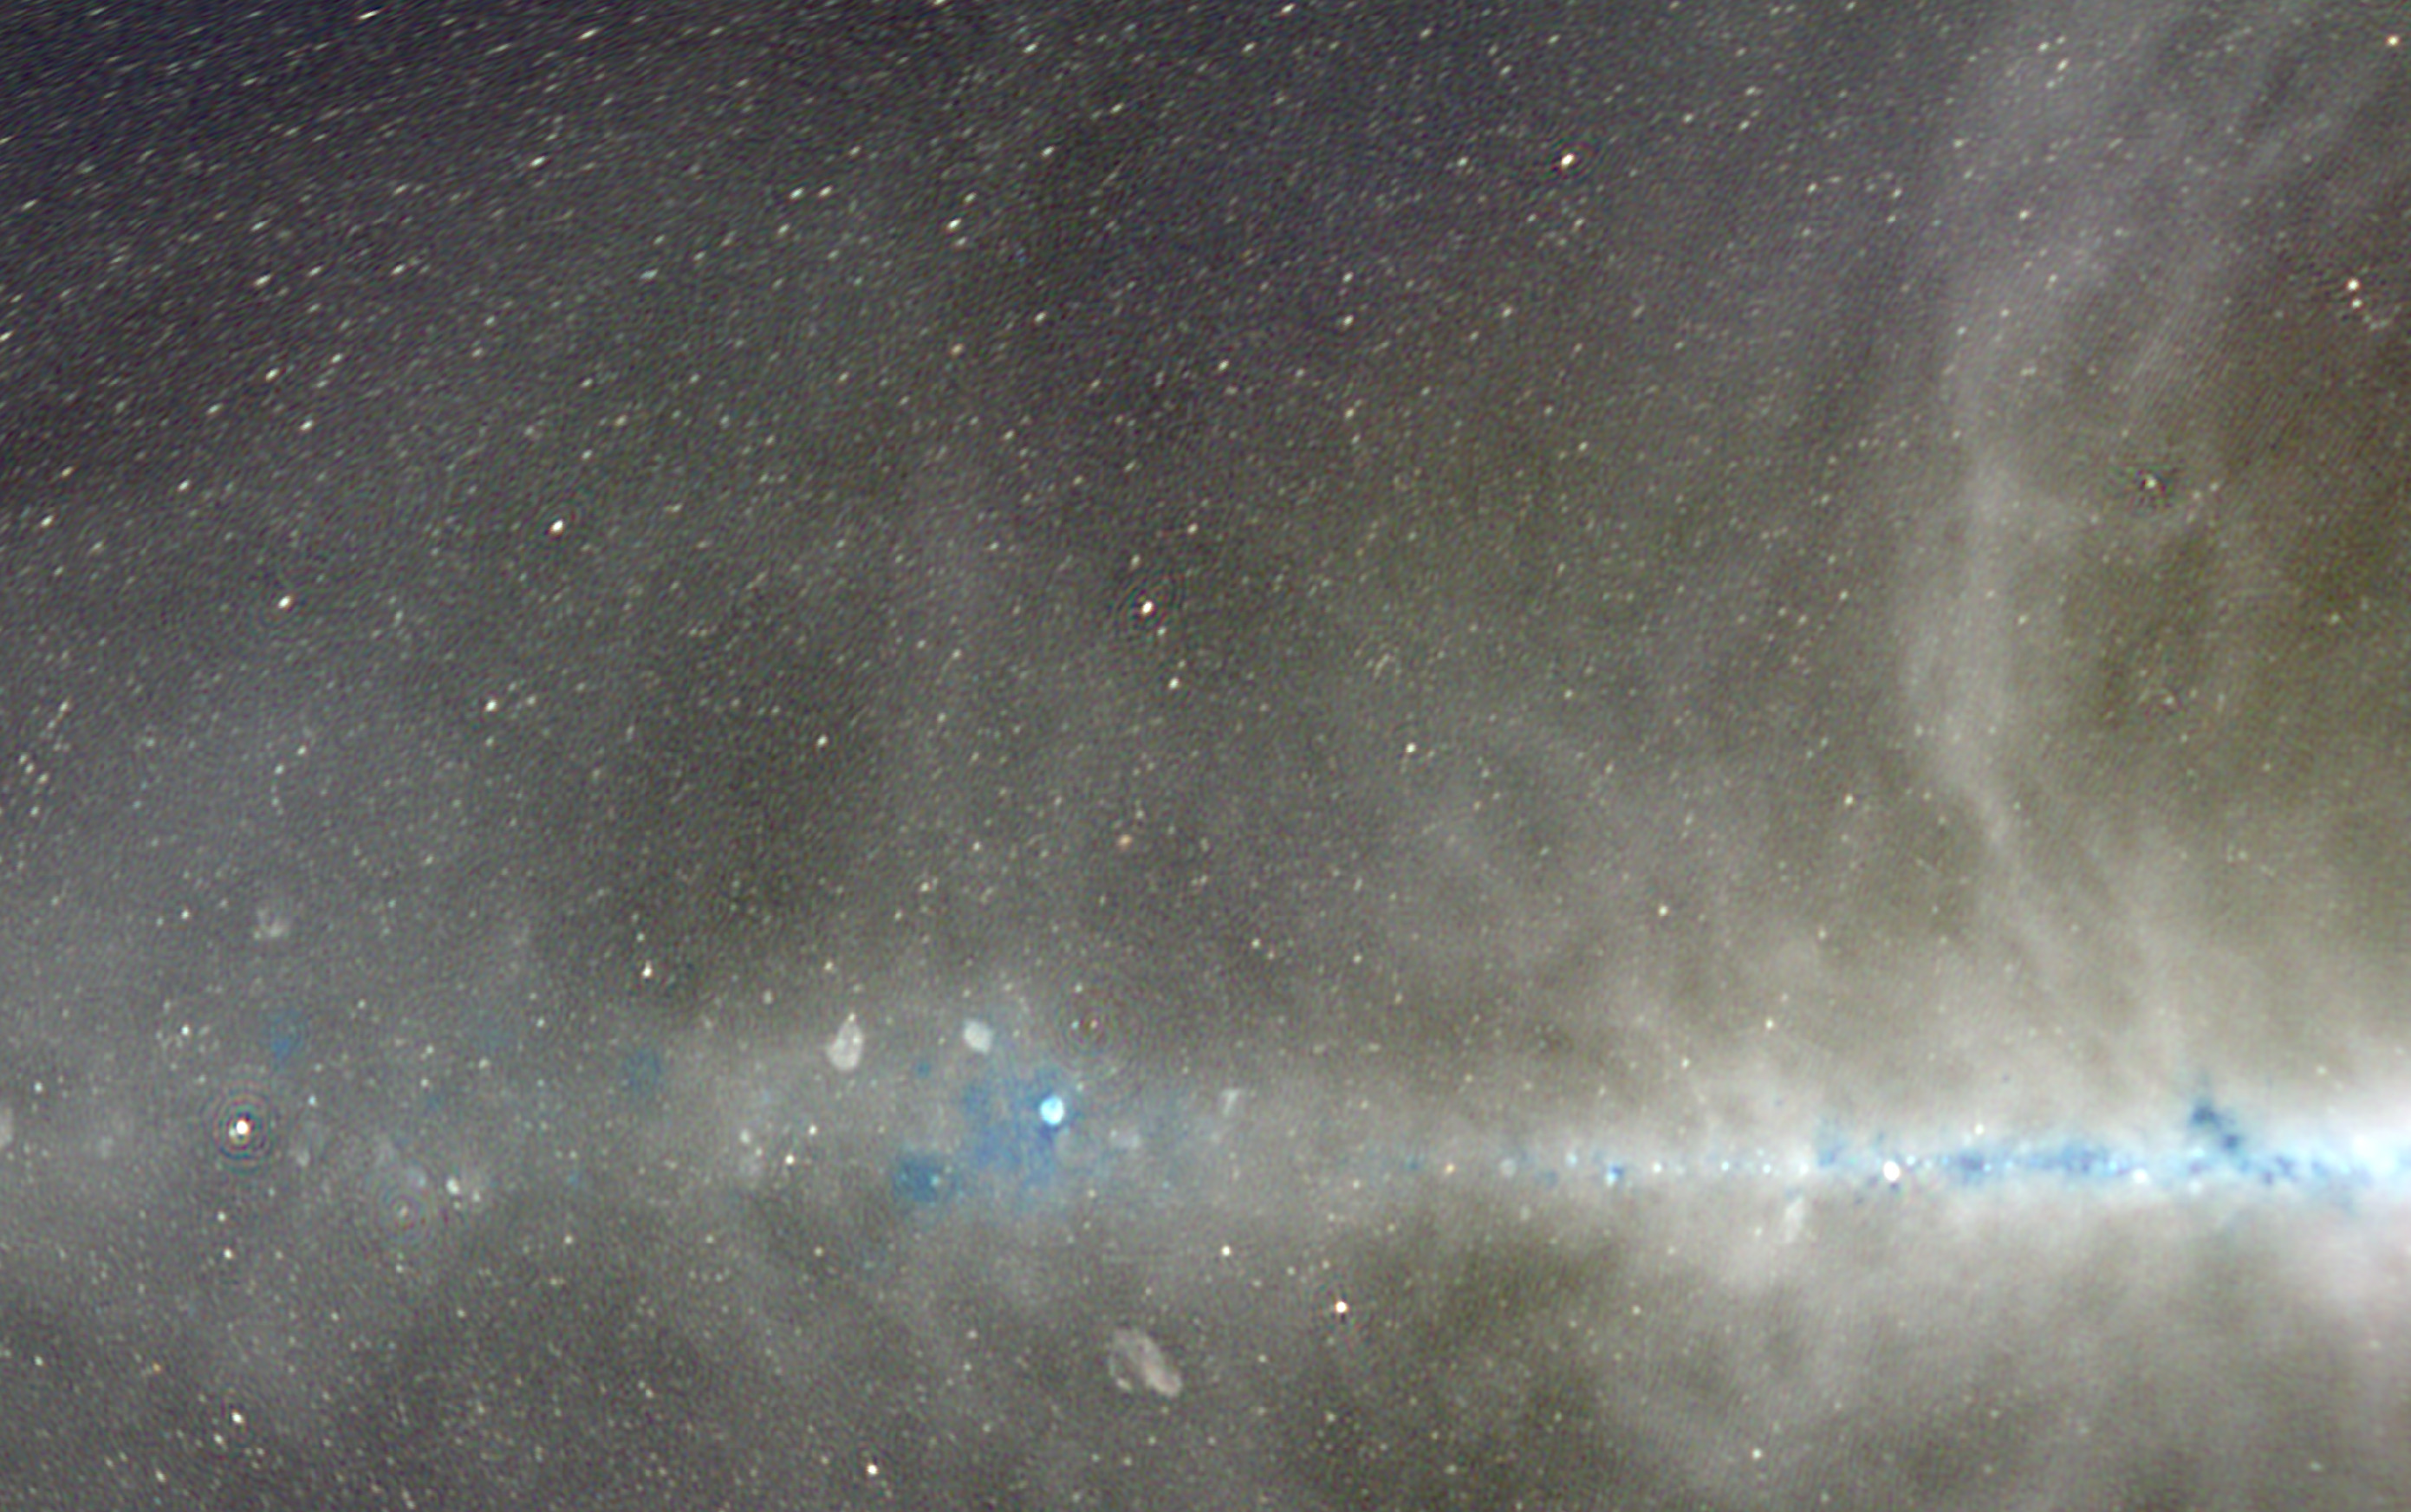
\includegraphics[height=\paperheight]{figures/title-slide.jpg}}
    \begin{frame}[t]
        \begin{center}
            \textbf{
                \Large
                Searching for the Cosmic Dawn with the\\
                \vskip4pt
                \large
                Hyperfine Structure Transition of Hydrogen
            } \\
            \vskip8pt
            \hrule
            \vskip8pt
            \textbf{Michael W. Eastwood} \\
            {\footnotesize \textbf{Thesis Defense}} \\
            {\footnotesize September 3, 2018} \\
        \end{center}
    \end{frame}
}

\begin{frame}
    \begin{columns}[t]
        \begin{column}{0.1\textwidth}
        \end{column}
        \begin{column}{0.4\textwidth}
            \begin{itemize}[leftmargin=0in]
                \item[] \textbf{Caltech}
                    \begin{itemize}[leftmargin=0.5cm]
                        \item[] {\footnotesize \color{yellow} Gregg Hallinan}
                        \item[] {\footnotesize Sandy Weinreb}
                        \item[] {\footnotesize Larry D'Addario}
                        \item[] {\footnotesize Stephen Bourke} {\tiny $\rightarrow$ Chalmers}
                        \item[] {\footnotesize Jake Hartman} {\tiny $\rightarrow$ Google}
                        \item[] {\footnotesize Harish Vedantham}
                        \item[] {\footnotesize Jonathon Kocz}
                        \item[] {\footnotesize Kate Clark}
                        \item[] {\footnotesize \color{yellow} Marin Anderson}
                        \item[] {\footnotesize \color{yellow} Ryan Monroe}
                        \item[] {\footnotesize Devin Cody}
                        \item[] {\footnotesize David Wang}
                    \end{itemize}
            \end{itemize}
        \end{column}
        \begin{column}{0.4\textwidth}
            \begin{itemize}[leftmargin=0in]
                \item[] \textbf{Harvard/SAO}
                    \begin{itemize}[leftmargin=0.5cm]
                        \item[] {\footnotesize Lincoln Greenhill}
                        \item[] {\footnotesize Ben Barsdell} {\tiny $\rightarrow$ NVIDIA}
                        \item[] {\footnotesize Danny Price} {\tiny $\rightarrow$ Swinburne}
                        \item[] {\footnotesize Hugh Garsden}
                        \item[] {\footnotesize Gianni Bernardi} {\tiny $\rightarrow$ SKA}
                    \end{itemize}
                \item[] \textbf{OVRO}
                    \begin{itemize}[leftmargin=0.5cm]
                        \item[] {\footnotesize David Woody}
                        \item[] {\footnotesize James Lamb}
                        \item[] {\footnotesize OVRO staff}
                    \end{itemize}
                \item[] \textbf{JPL}
                    \begin{itemize}[leftmargin=0.5cm]
                        \item[] {\footnotesize Joe Lazio}
                    \end{itemize}
                \item[] {\footnotesize and the rest of the LWA team}
            \end{itemize}
        \end{column}
        \begin{column}{0.1\textwidth}
        \end{column}
    \end{columns}
\end{frame}

\begin{frame}

    {\Large \bfseries This Thesis}
    \vskip8pt
    \hrule
    \vskip8pt
    \begin{enumerate}
        \item[I.] Introduction to 21\,cm Cosmology
        \item[II.] Commissioning the OVRO-LWA
        \item[III.] New Maps of the Sky at Meter Wavelengths
        \item[IV.] Upper Limits on the 21\,cm Power Spectrum ($z>18$)
    \end{enumerate}
\end{frame}

%%%%%%%%%%%%%%%%%%%%%%%%%%%%%%%%%%%%%%%%%%%%%%%%%%%%%%%%%%%%%%%%%%%%%%%%%%%%%%%%%%%%%%%%%%%%%%%%%%%%

\section{I. Introduction}

{
    \usebackgroundtemplate{
\includegraphics[height=\paperheight]{figures/waves1}}
    \begin{frame}[t]

        {\large \bfseries I. Introduction to 21\,cm Cosmology}
    \end{frame}
}

\begin{frame}
    \begin{center}
        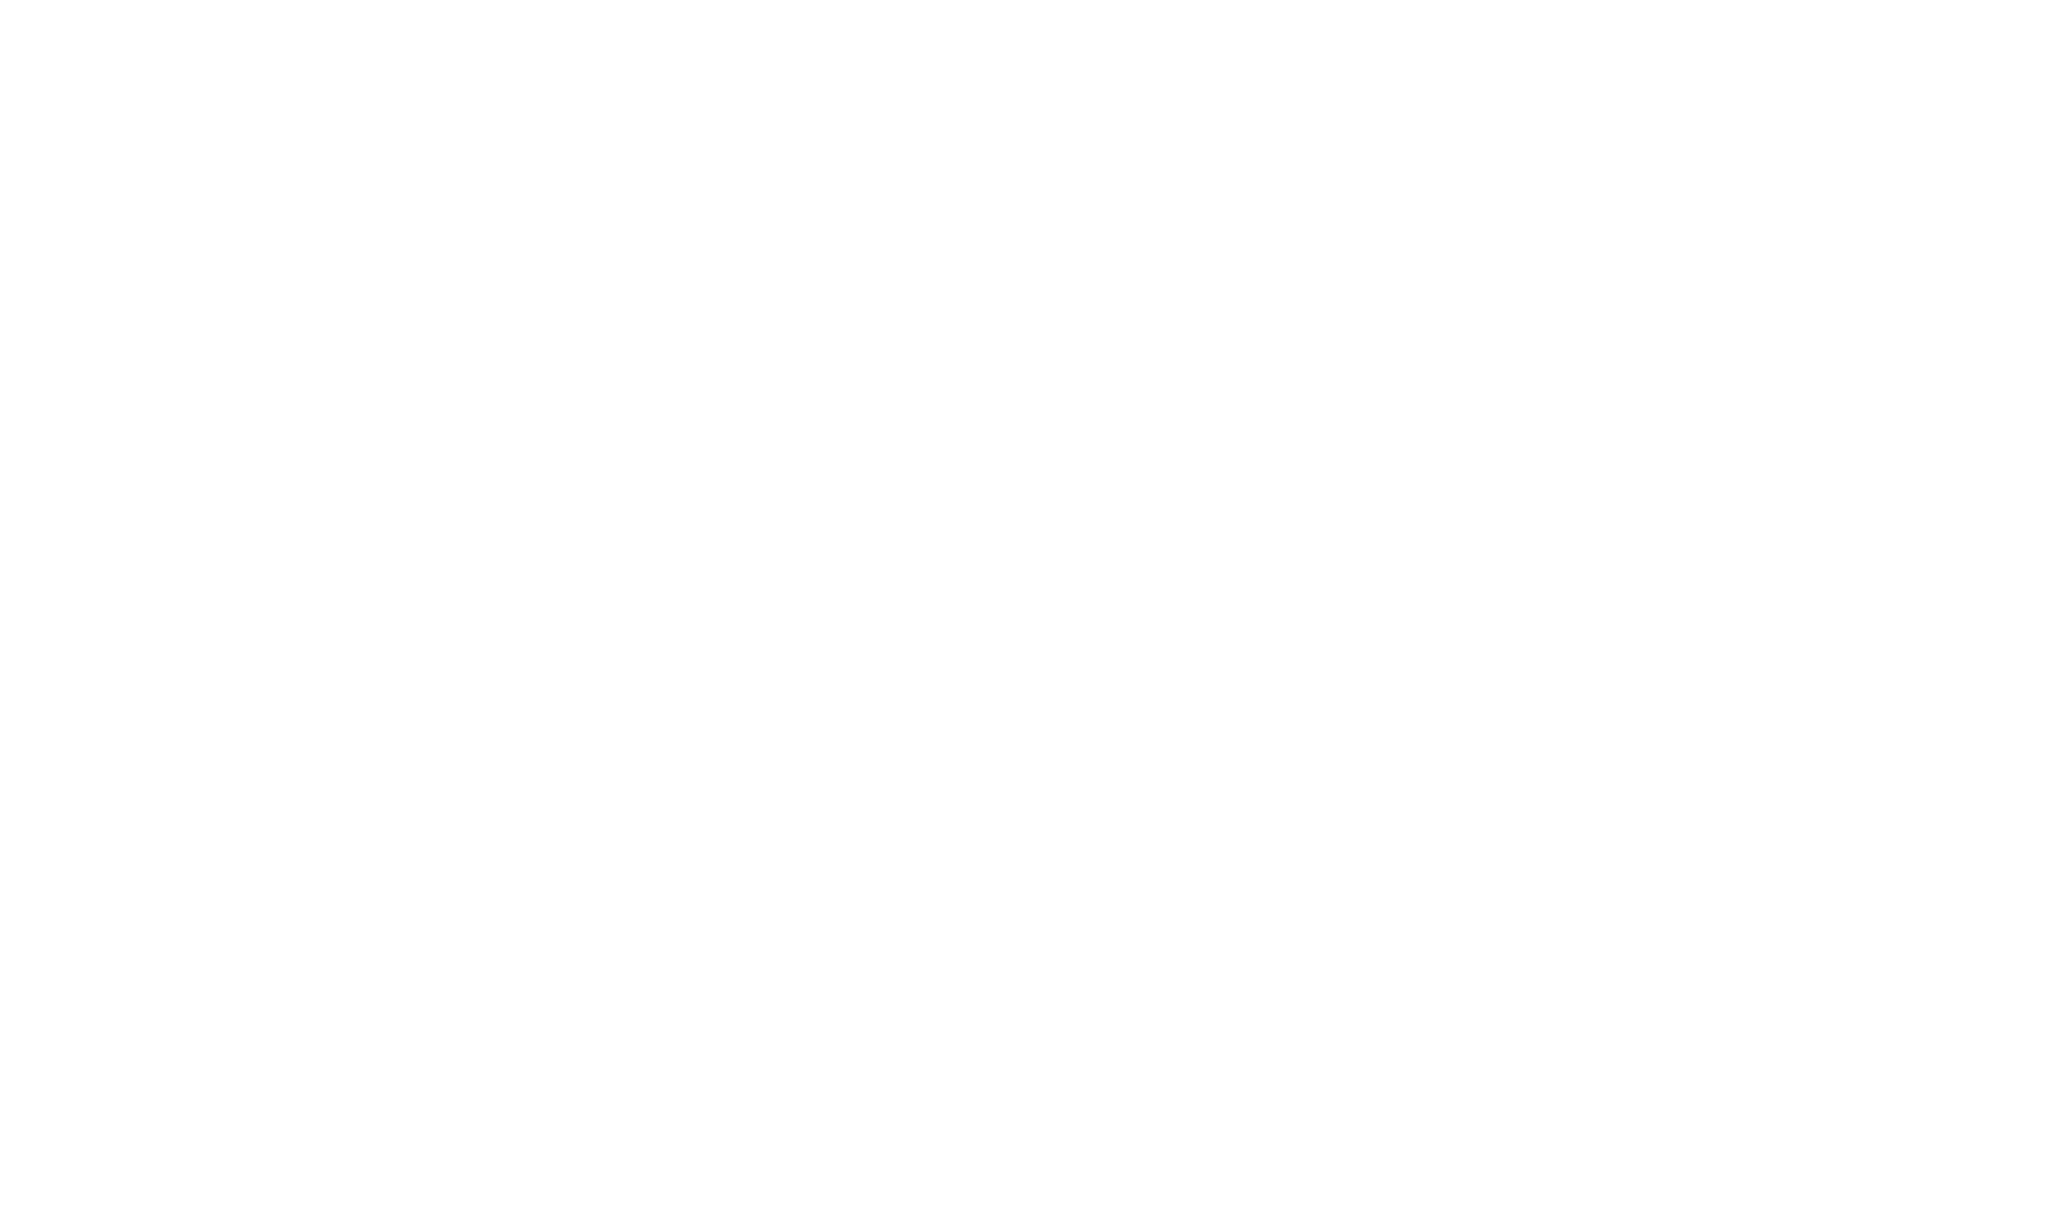
\includegraphics[width=\textwidth]{figures/2df}
    \end{center}
    \begin{center}
        \tiny{Colless et al. (2001)}
    \end{center}
\end{frame}

{
    \usebackgroundtemplate{\includegraphics[width=\paperwidth]{figures/hudf}}
    \begin{frame}\end{frame}
}

{
    \usebackgroundtemplate{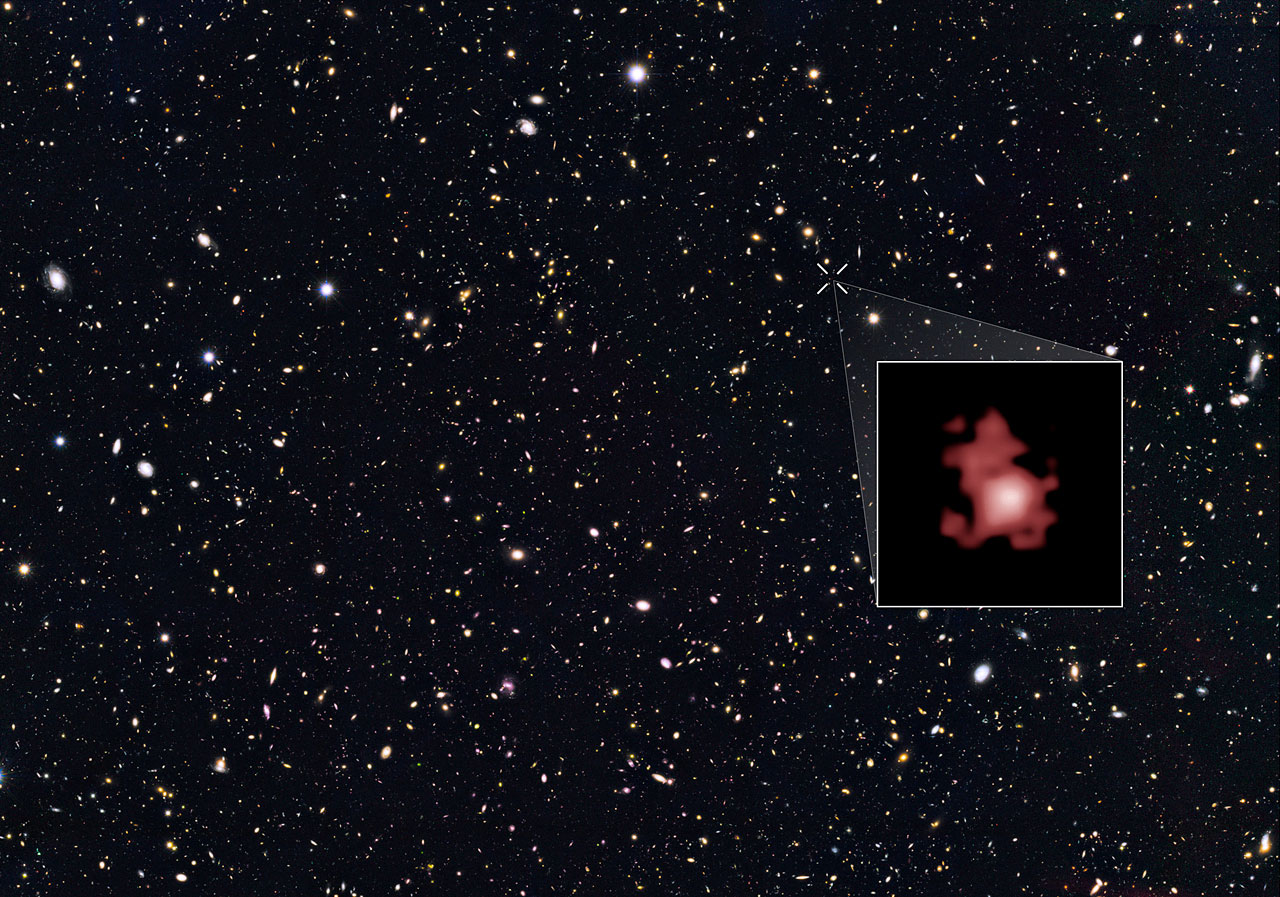
\includegraphics[height=\paperheight]{figures/oesch-gn-z11}}
    \begin{frame}\end{frame}
}

\begin{frame}
    \begin{overprint}
        \onslide<1>
        \begin{center}
            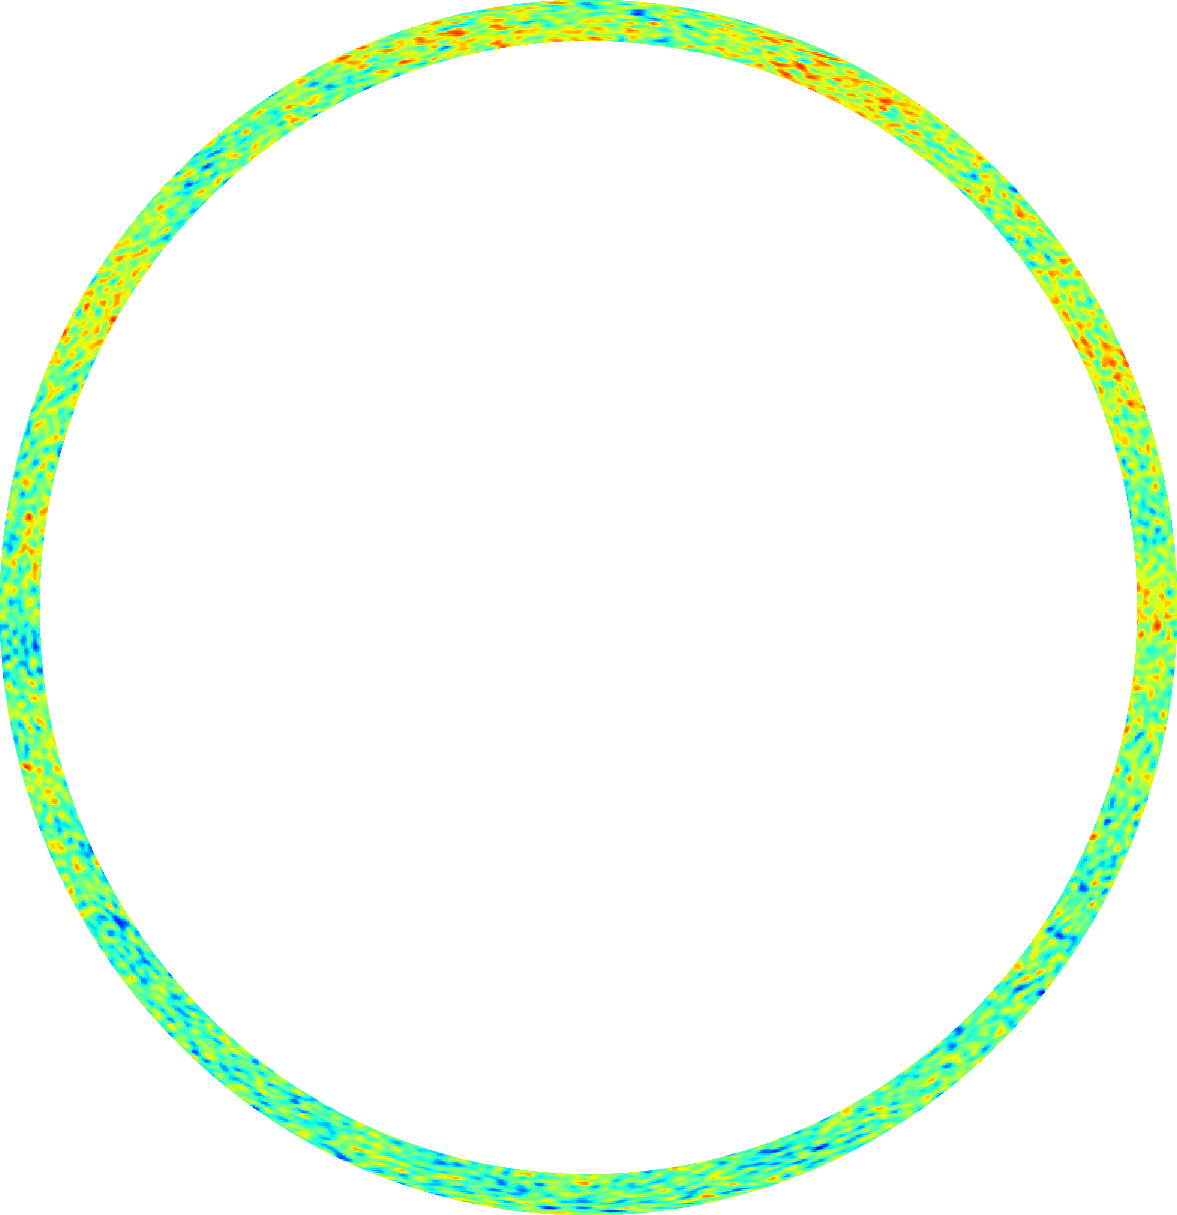
\includegraphics[height=\textheight]{figures/scalemap1}
        \end{center}
        \onslide<2>
        \begin{center}
            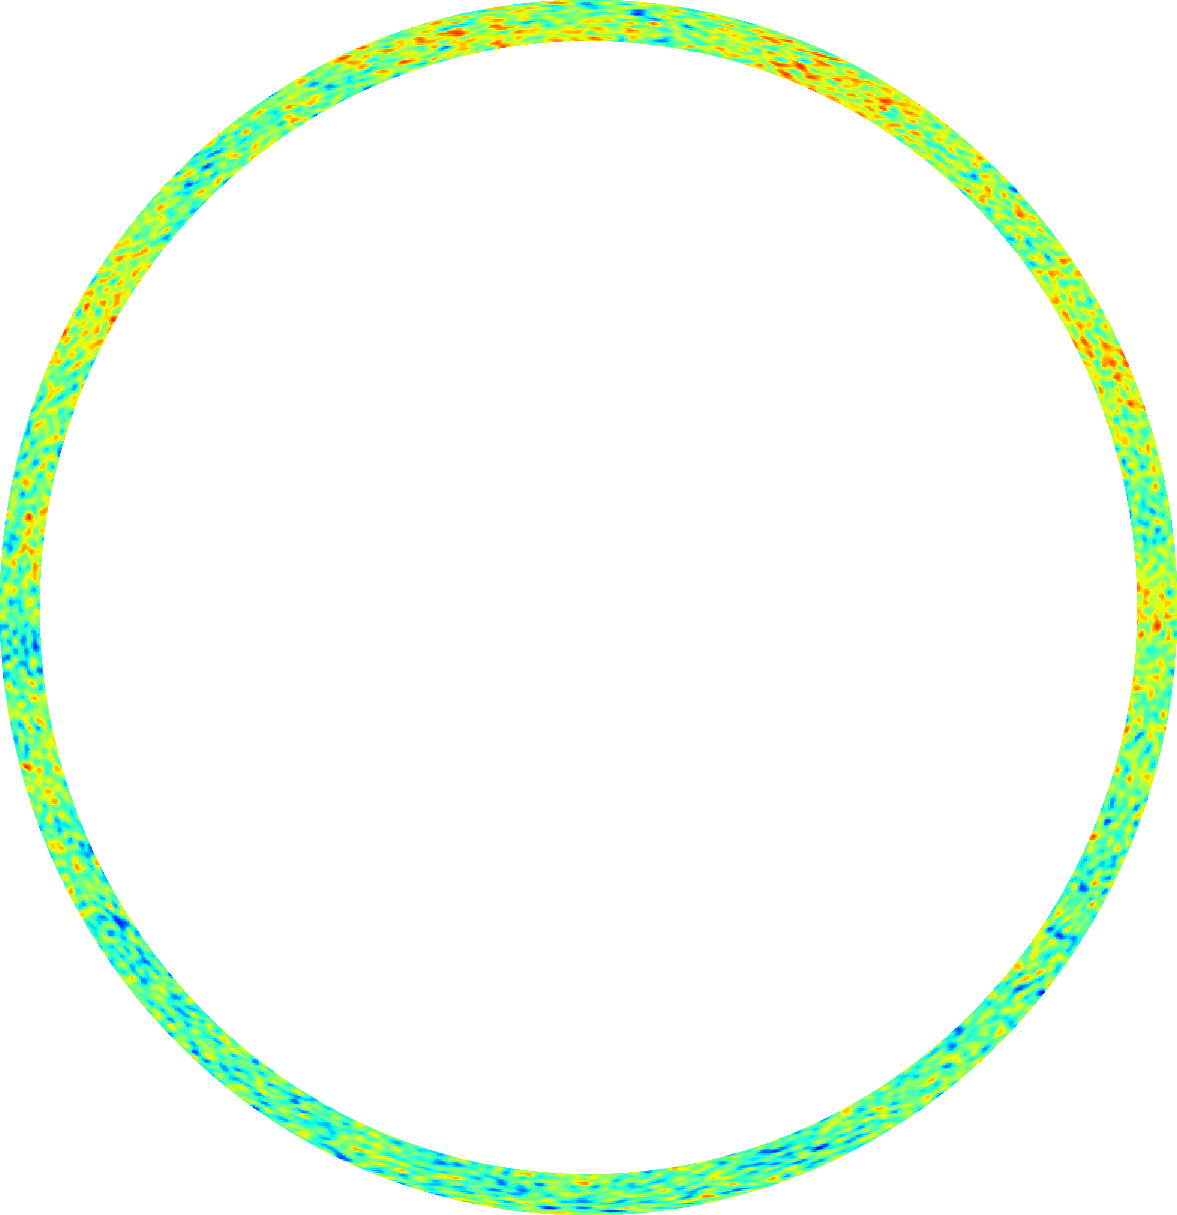
\includegraphics[height=\textheight]{figures/scalemap3} % out of order by choice
        \end{center}
        \onslide<3>
        \begin{center}
            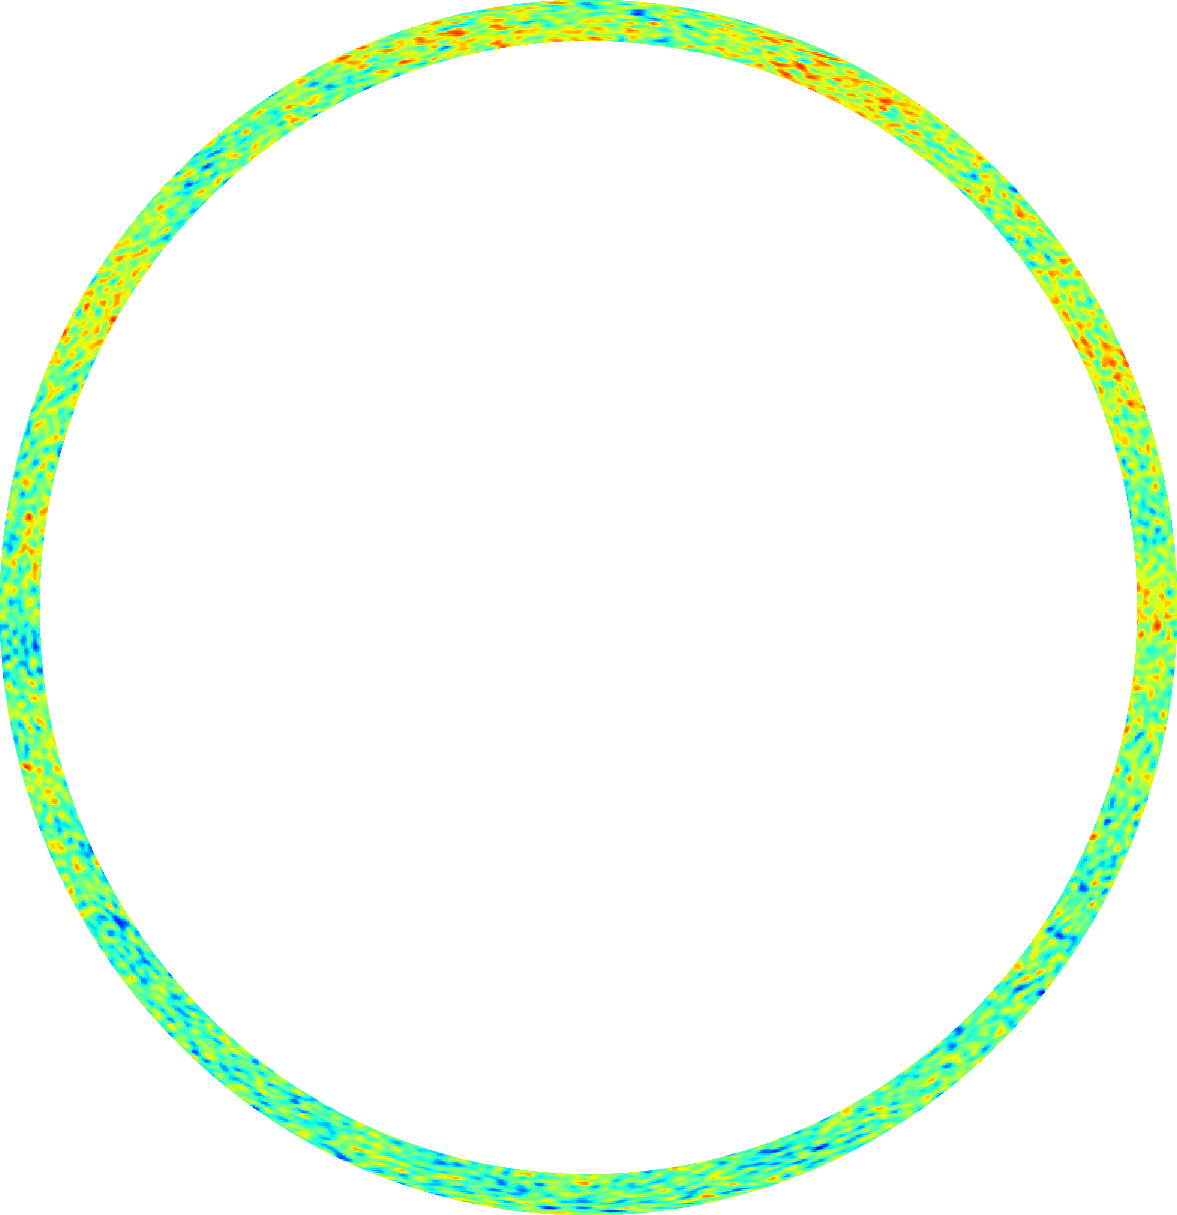
\includegraphics[height=\textheight]{figures/scalemap2} % out of order by choice
        \end{center}
        \onslide<4>
        \begin{center}
            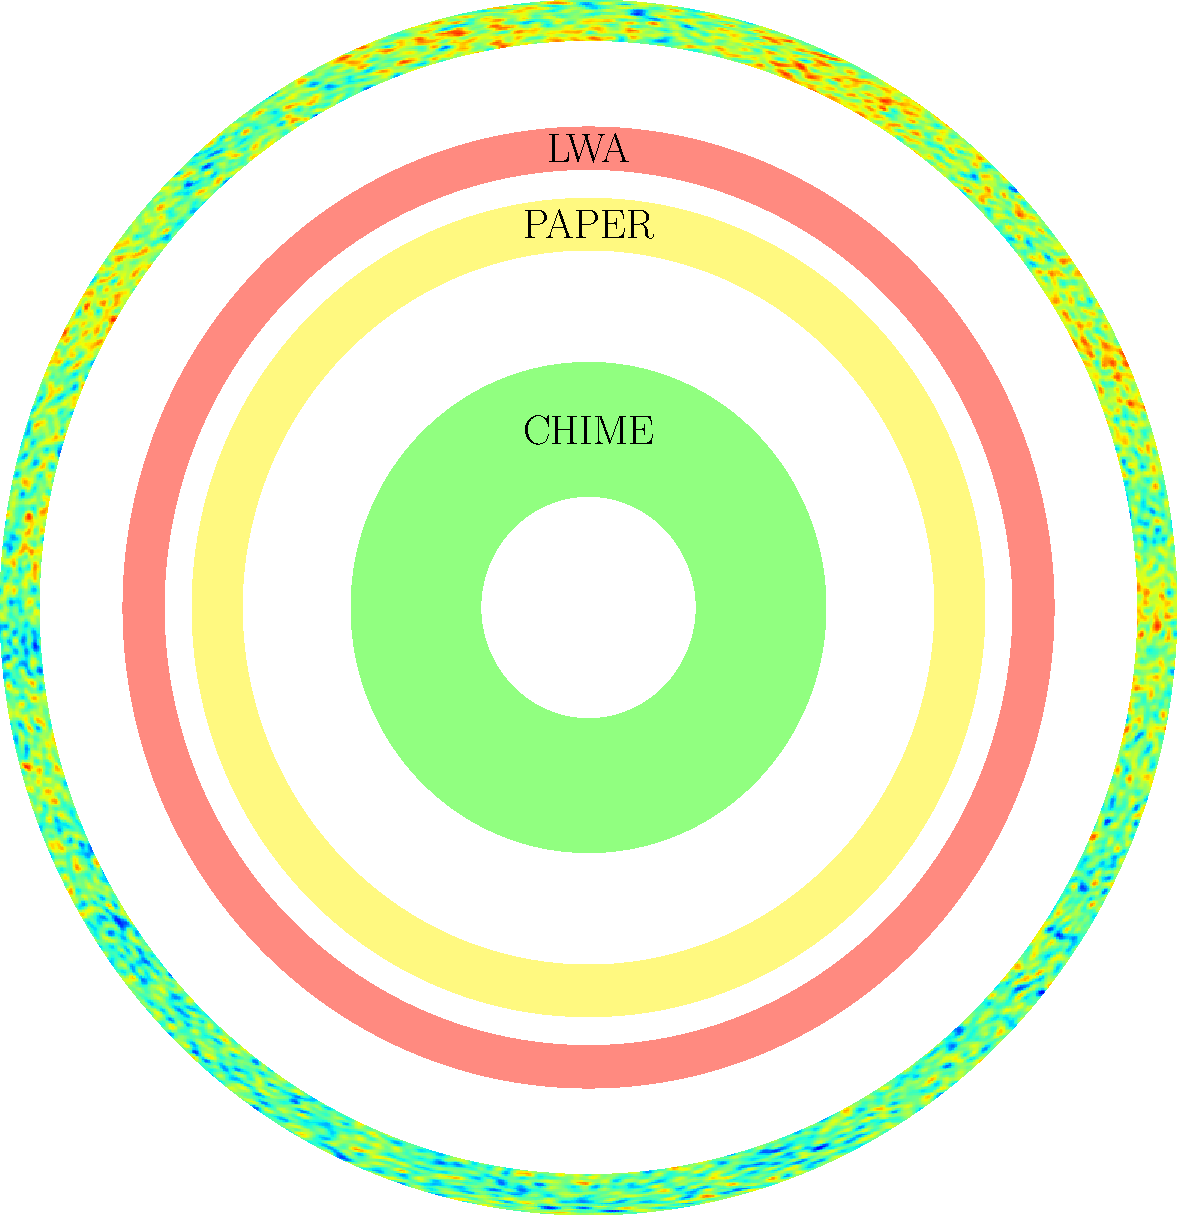
\includegraphics[height=\textheight]{figures/scalemap4}
        \end{center}
    \end{overprint}
\end{frame}

\begin{frame}{Hyperfine Structure}
    \begin{center}
        
\includegraphics[width=0.8\textwidth]{figures/finestructure}
    \end{center}
    \begin{itemize}[label=\textbullet, leftmargin=5em]
        \item Magnetic dipole transition $\rightarrow$ very weak
        \item Optically thin tracer of HI
        \item Spin temperature $\sim$ excitation state
    \end{itemize}
\end{frame}

\begin{frame}{Radiative Transfer}
    \begin{center}
        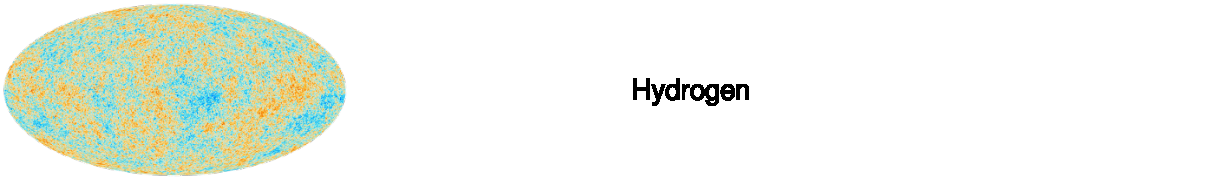
\includegraphics[width=\textwidth]{figures/radiative-transfer}
    \end{center}
    \begin{dmath*}
        T_{21} \sim 27 \left[
            \overbrace{
                x_{\rm HI} (1+\delta)
                \left(\frac{\Omega_b h}{0.0327}\right)
            }^{\text{quantity of HI}}
            \left(\frac{\Omega_m}{0.307}\right)^{-1/2}
            \left(\frac{1+z}{10}\right)^{1/2} \linebreak \times
            \underbrace{
                \left(\frac{T_{\rm spin} - T_{\rm CMB}(z)}{T_{\rm spin}}\right)
            }_{\text{relative temperature}}
        \right] \, {\rm mK}
    \end{dmath*}
    \begin{center}
        \tiny{Pritchard \& Loeb (2012)}
    \end{center}
\end{frame}

\begin{frame}{Cooling}
    \begin{center}
        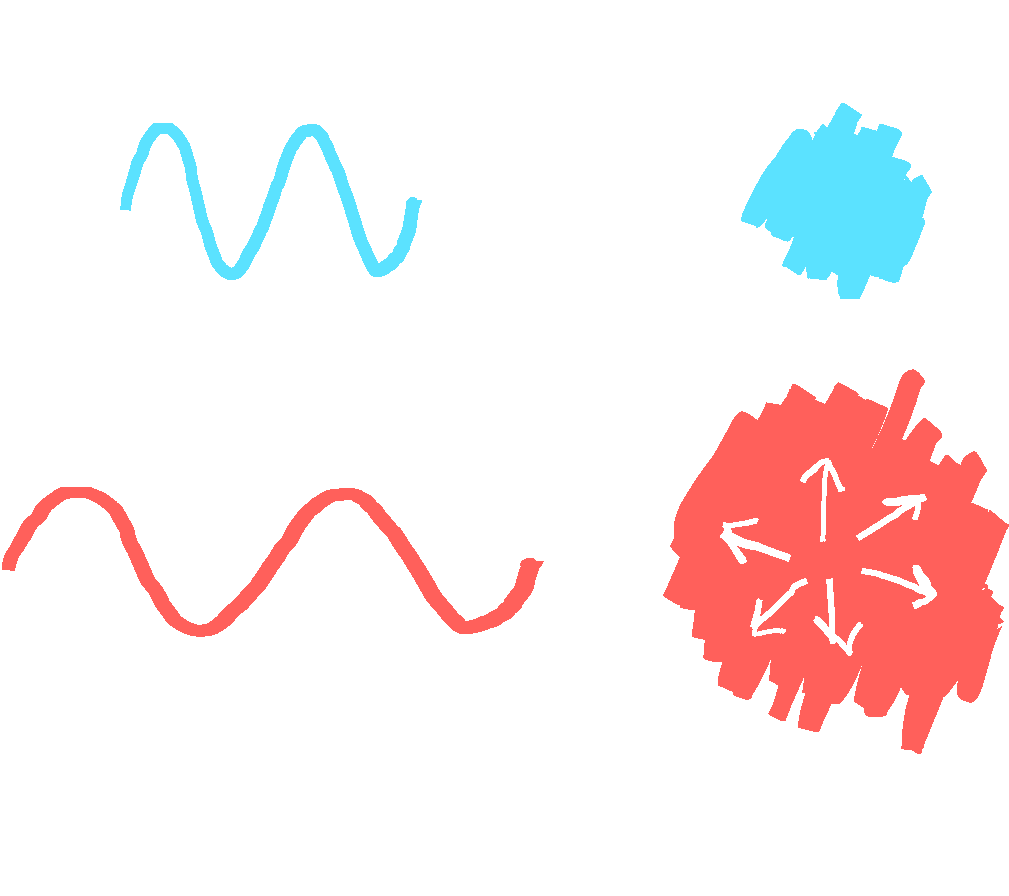
\includegraphics[height=0.6\textheight]{figures/expansion}
    \end{center}
\end{frame}

\begin{frame}{Temperature History}
    \begin{overprint}
        % note that there is no thermal-history-1
        \onslide<1>
        \begin{center}
            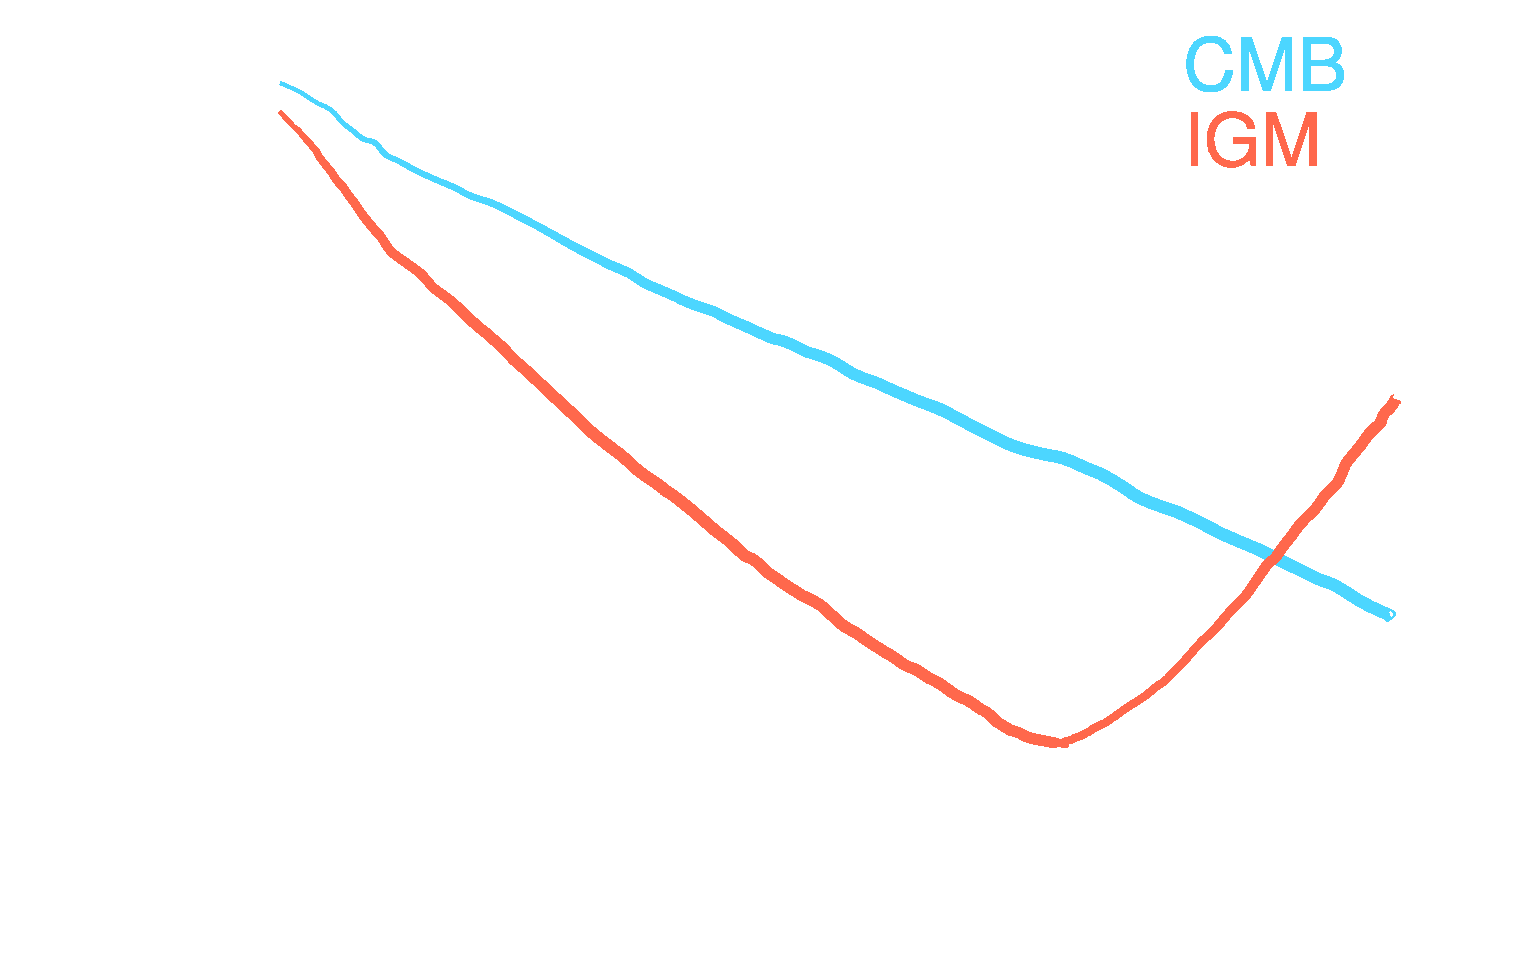
\includegraphics[height=0.6\textheight]{figures/thermal-history-2}
        \end{center}
        \onslide<2>
        \begin{center}
            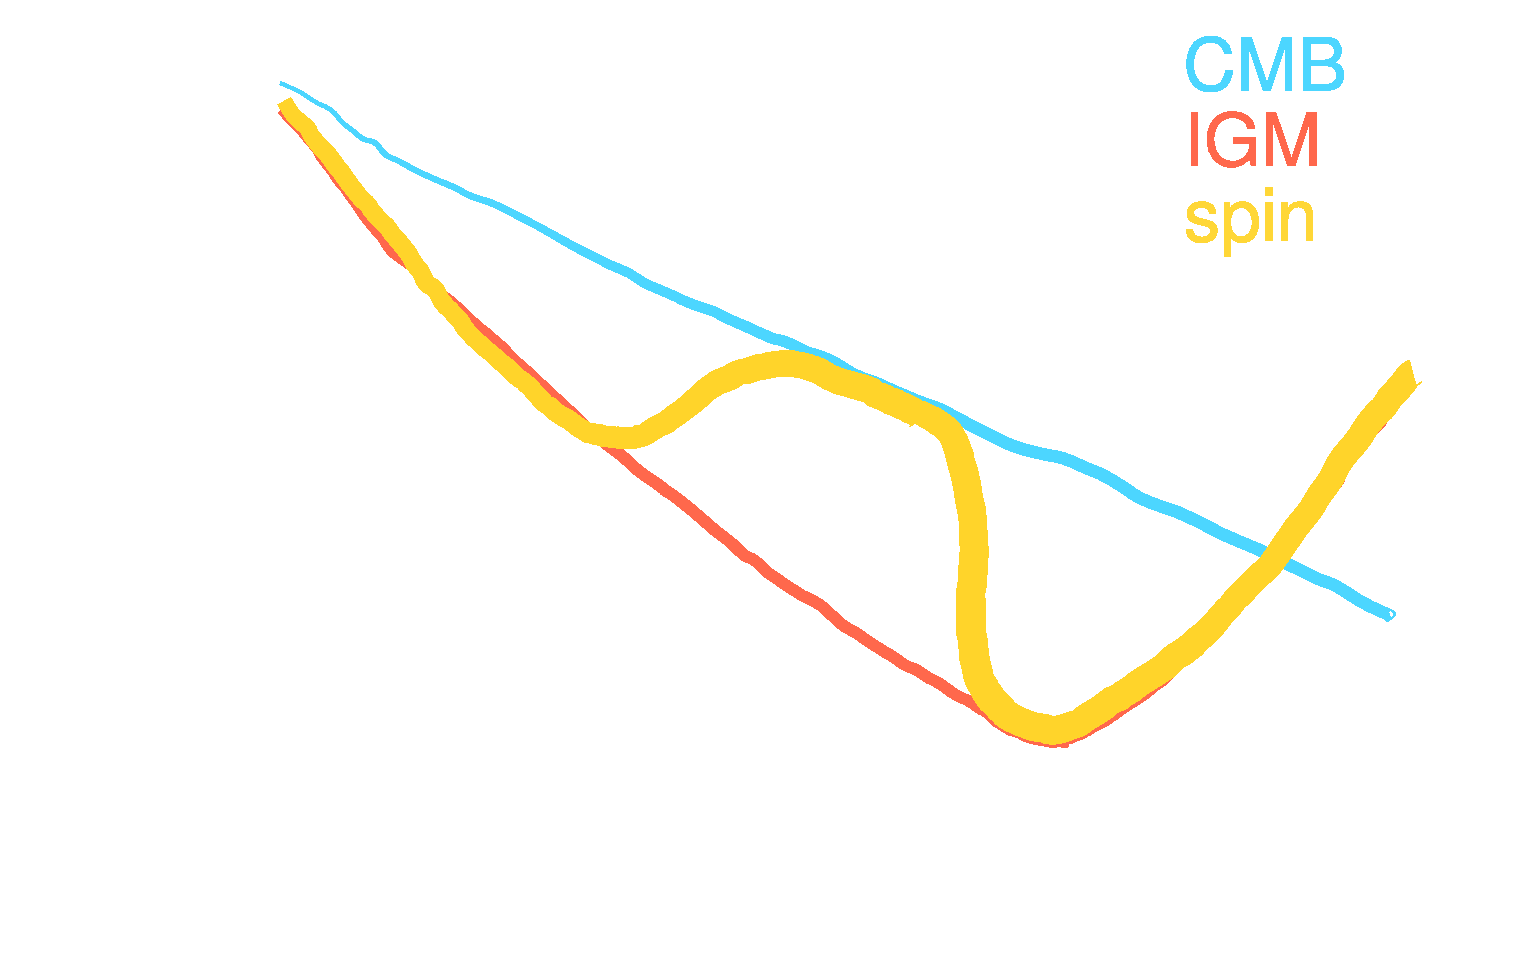
\includegraphics[height=0.6\textheight]{figures/thermal-history-3}
        \end{center}
        \onslide<3>
        \begin{center}
            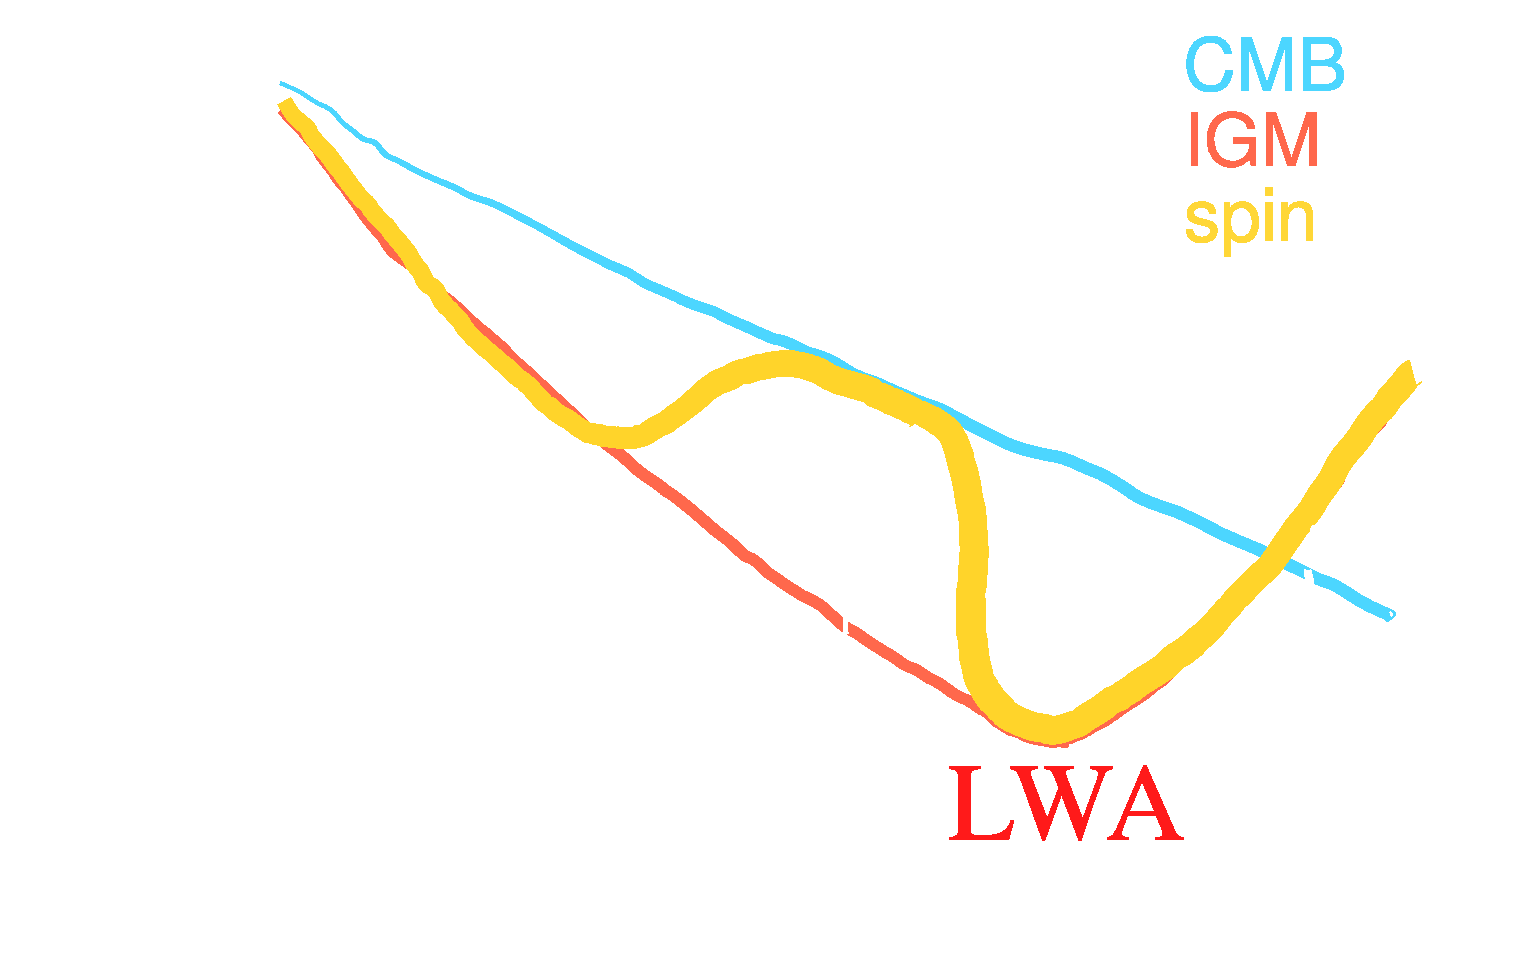
\includegraphics[height=0.6\textheight]{figures/thermal-history-4}
        \end{center}
    \end{overprint}
\end{frame}

{
    \usebackgroundtemplate{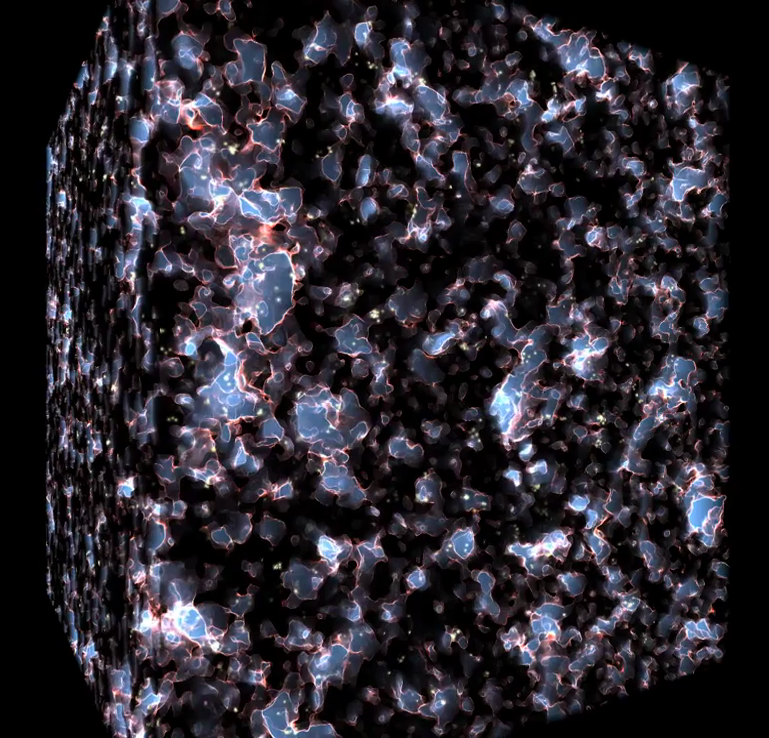
\includegraphics[width=\paperwidth]{movies/alvarez-cosmic-reionization}}
    \begin{frame}[b]
        \begin{tikzpicture}[overlay, remember picture]
            \node[anchor=center] at (current page.center) {
                \href{run:movies/alvarez-cosmic-reionization.mp4} {
                    
\includegraphics[width=30pt]{movies/play-button}
                }
            };
        \end{tikzpicture}
        \begin{center}
            \tiny{Alvarez et al. (2009)}
        \end{center}
    \end{frame}
}

\begin{frame}{The 3D Spatial Power Spectrum}
    \begin{center}
        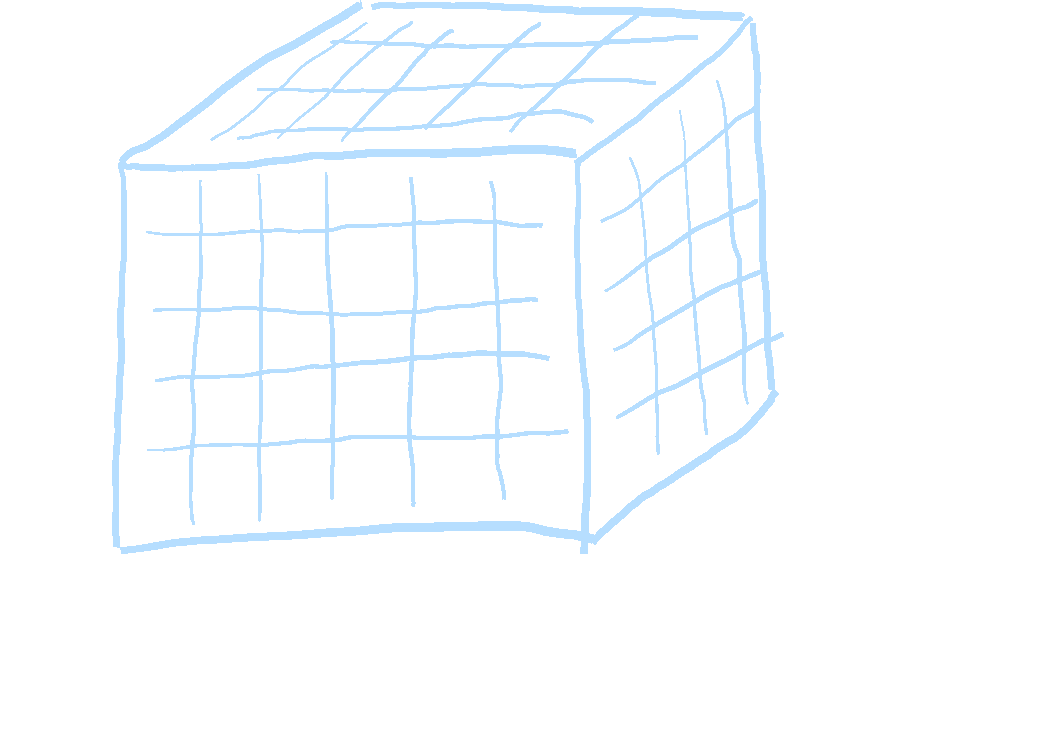
\includegraphics[height=0.5\textheight]{figures/cube}
    \end{center}
    Fourier transform and square the brightness temperature in the cosmological cube.
\end{frame}

\begin{frame}{The 21 cm Signal}
    \hskip 2em
    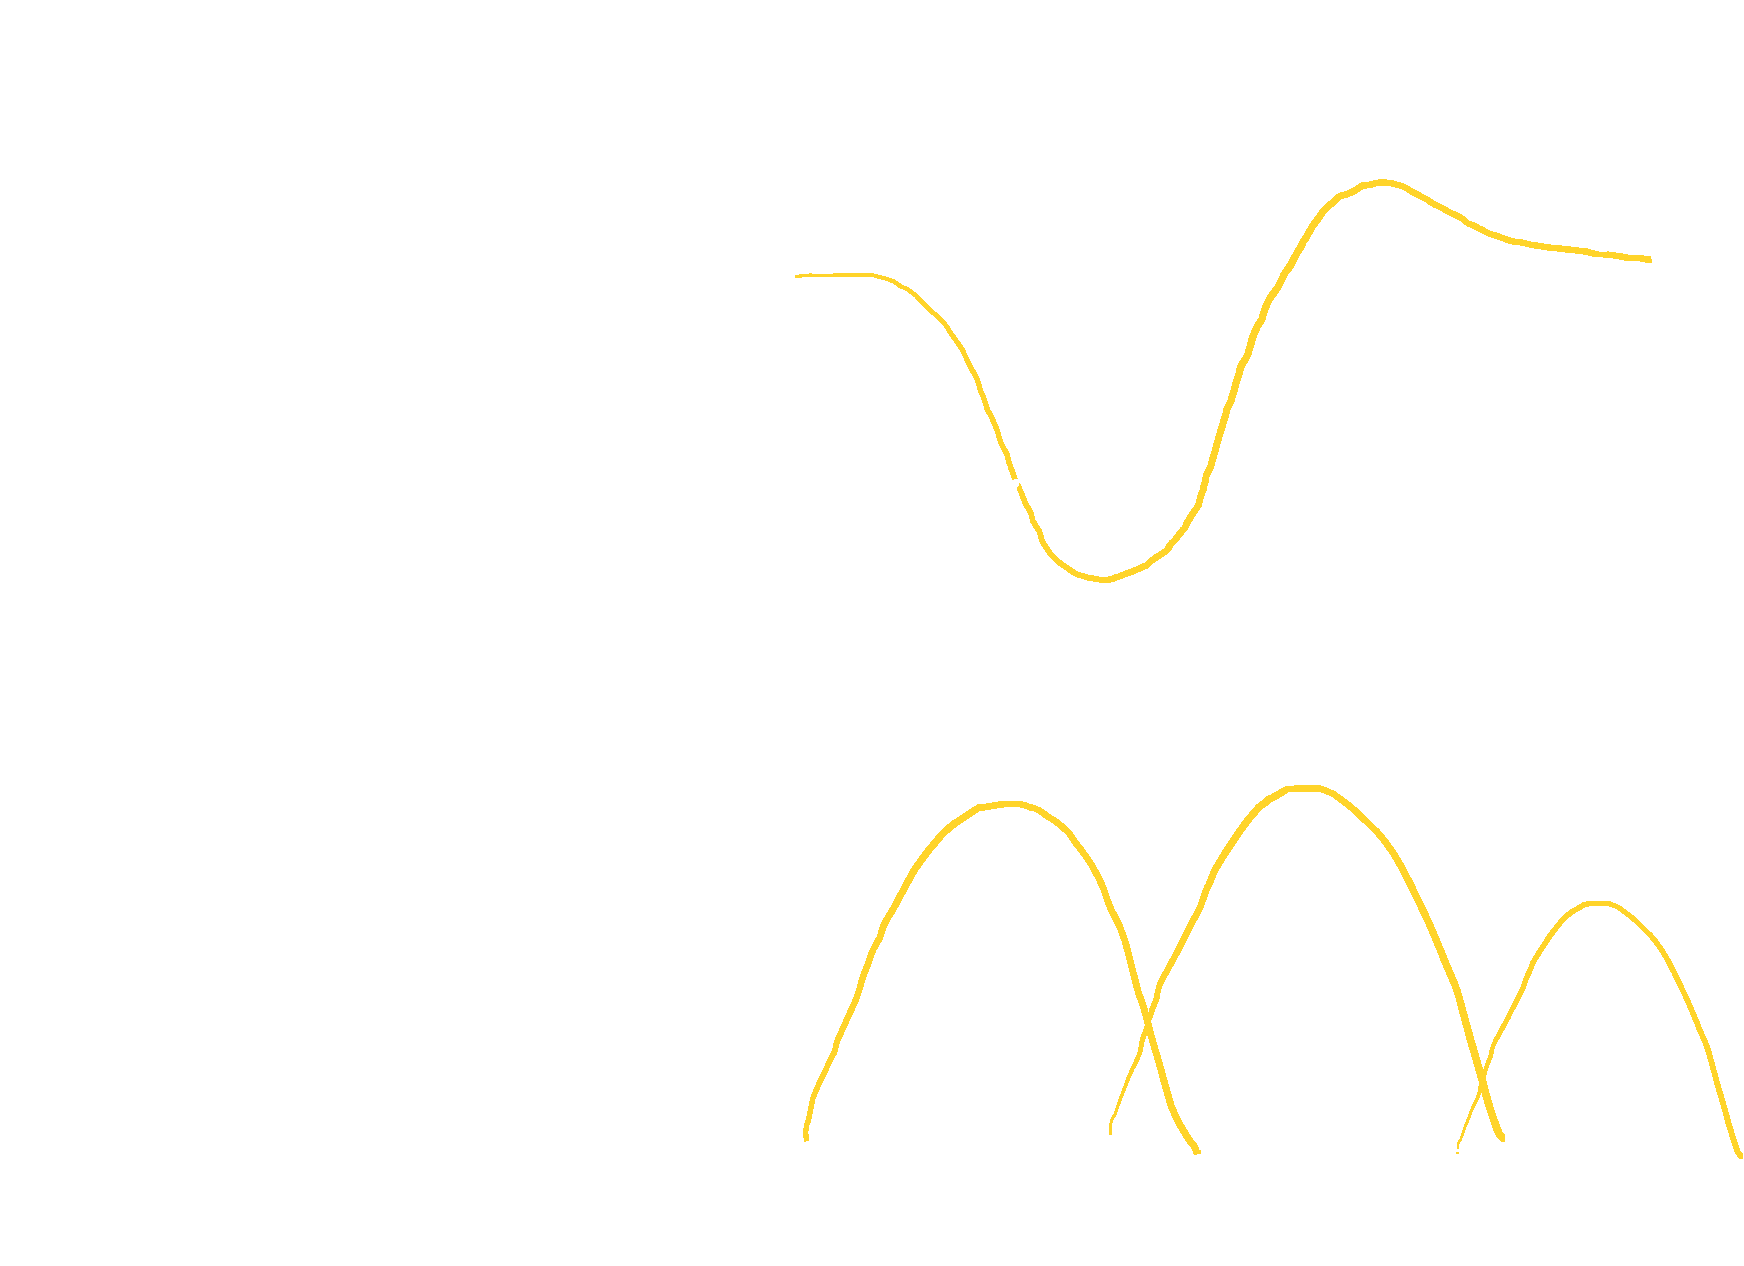
\includegraphics[height=0.8\textheight]{figures/21-cm-signal}
\end{frame}

\begin{frame}{Astrophysics from the Cosmic Dawn}
    Effects that influence the 21 cm signal \textbf{(pre-2018)}:
    \begin{itemize}[label=\textbullet]
        \item Timing of early star formation
        \item Inhomogeneous star formation
        \item Relative motion of baryons relative to dark matter\\
            {\tiny(Tseliakhovich \& Hirata 2010)}
        \item Lyman-Werner feedback\\
            {\tiny(Fialkov et al. 2013)}
        \item Flux and hardness of high-mass X-ray binaries\\
            {\tiny(Fialkov \& Barkana 2014)}
    \end{itemize}
\end{frame}

\begin{frame}
    \begin{center}
        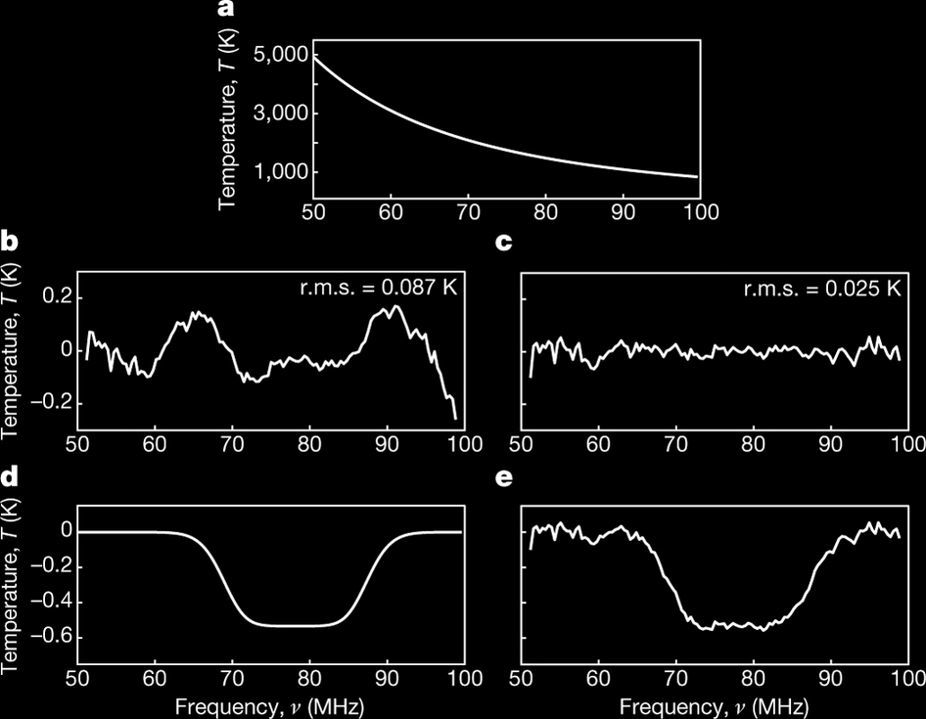
\includegraphics[height=0.9\textheight]{figures/bowman-2018-absorption-trough.jpg}
    \end{center}
    \begin{center}
        \tiny{Bowman et al. (2018)}
    \end{center}
\end{frame}

\begin{frame}{New Ideas}
    \begin{itemize}[label=\textbullet]
        \item Baryon--dark matter interactions\\
            {\tiny (Barkana 2018)}
        \item New population of high-redshift radio sources\\
            {\tiny (Ewall-Wice et al. 2018)}
        \item $\Omega_b = \Omega_m$
    \end{itemize}
    Generally, theoretical explanations of the Bowman et al. 2018 result predict an enhanced power
    spectrum amplitude ($\sim 7\times$).
\end{frame}

\begin{frame}
    \begin{center}
        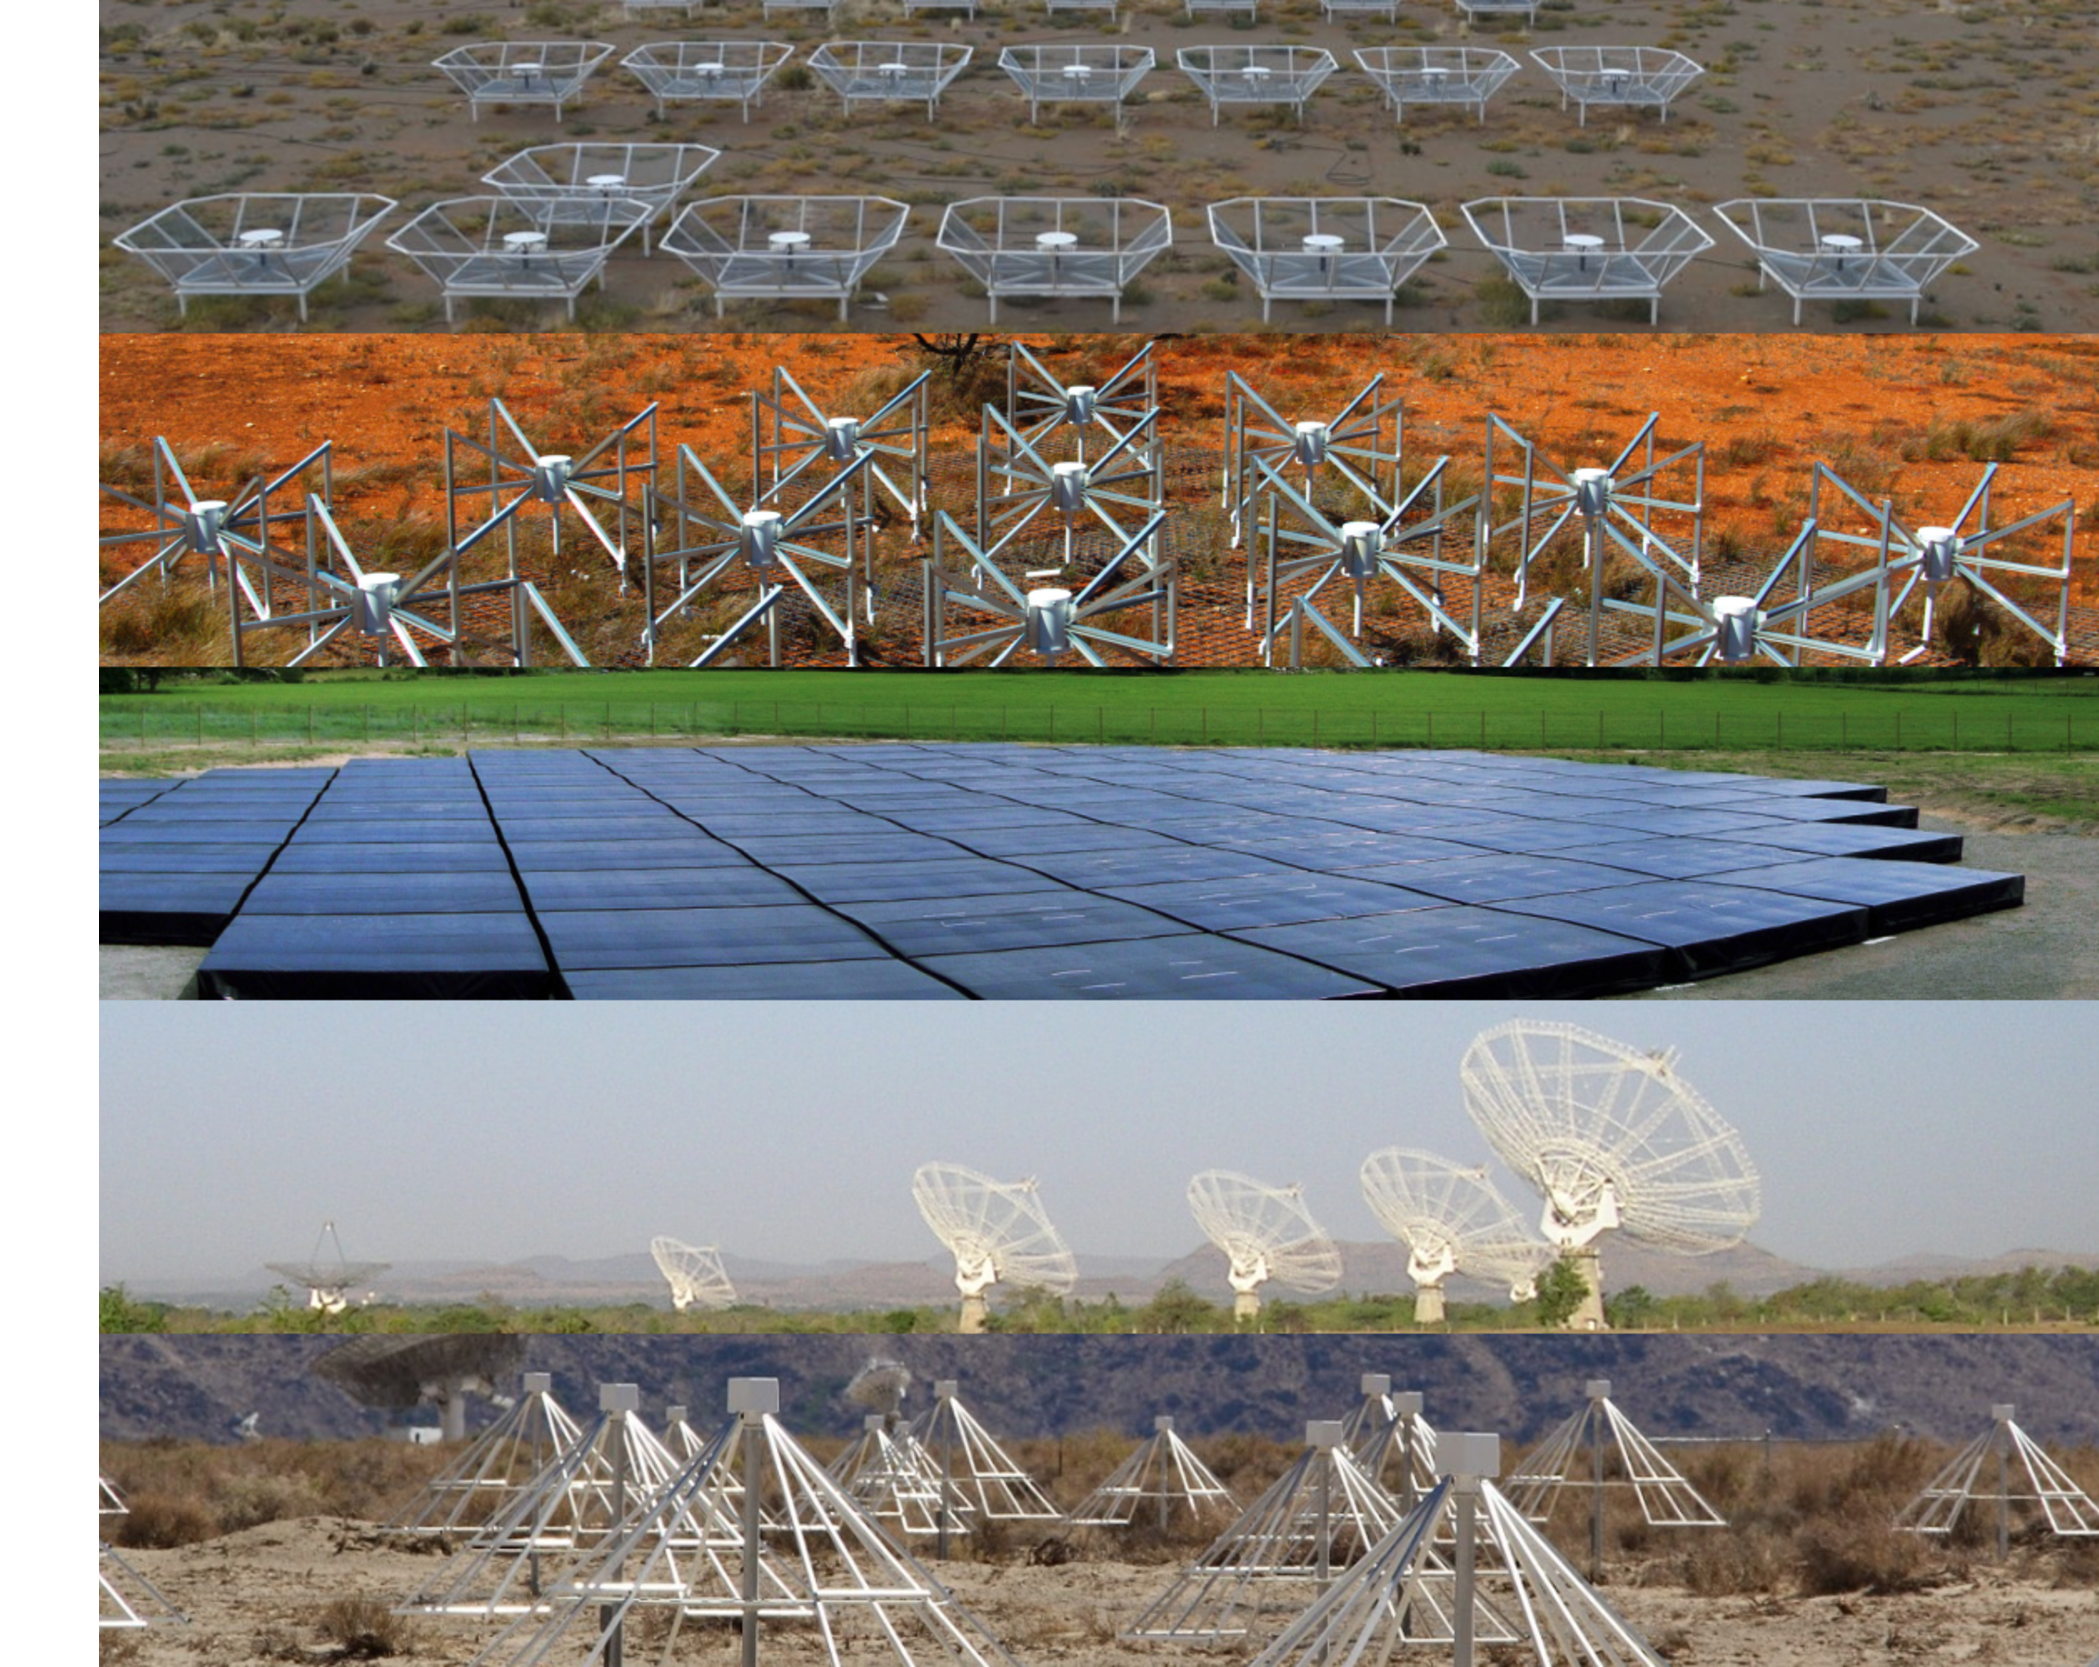
\includegraphics[width=0.9\textwidth]{figures/telescopes}
    \end{center}
\end{frame}

\begin{frame}{Power Spectrum Upper Limits}
    \begin{center}
        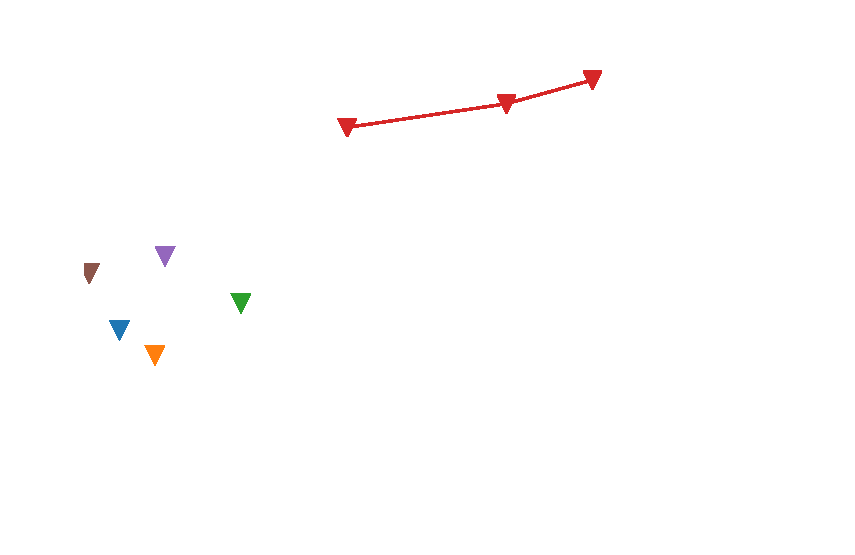
\includegraphics[height=0.75\textheight]{figures/power-spectrum-upper-limits/power-spectrum-upper-limits}
    \end{center}
\end{frame}

\begin{frame}{Foregrounds in 21 cm Cosmology}
    \begin{center}
        
\includegraphics[height=0.75\textheight]{figures/foregrounds}
    \end{center}
\end{frame}

%%%%%%%%%%%%%%%%%%%%%%%%%%%%%%%%%%%%%%%%%%%%%%%%%%%%%%%%%%%%%%%%%%%%%%%%%%%%%%%%%%%%%%%%%%%%%%%%%%%%

\section{II. The OVRO-LWA}

{
    \usebackgroundtemplate{
\includegraphics[height=\paperheight]{figures/waves2}}
    \begin{frame}[t]

        {\large \bfseries II. Commissioning the OVRO-LWA}
    \end{frame}
}

{
    \usebackgroundtemplate{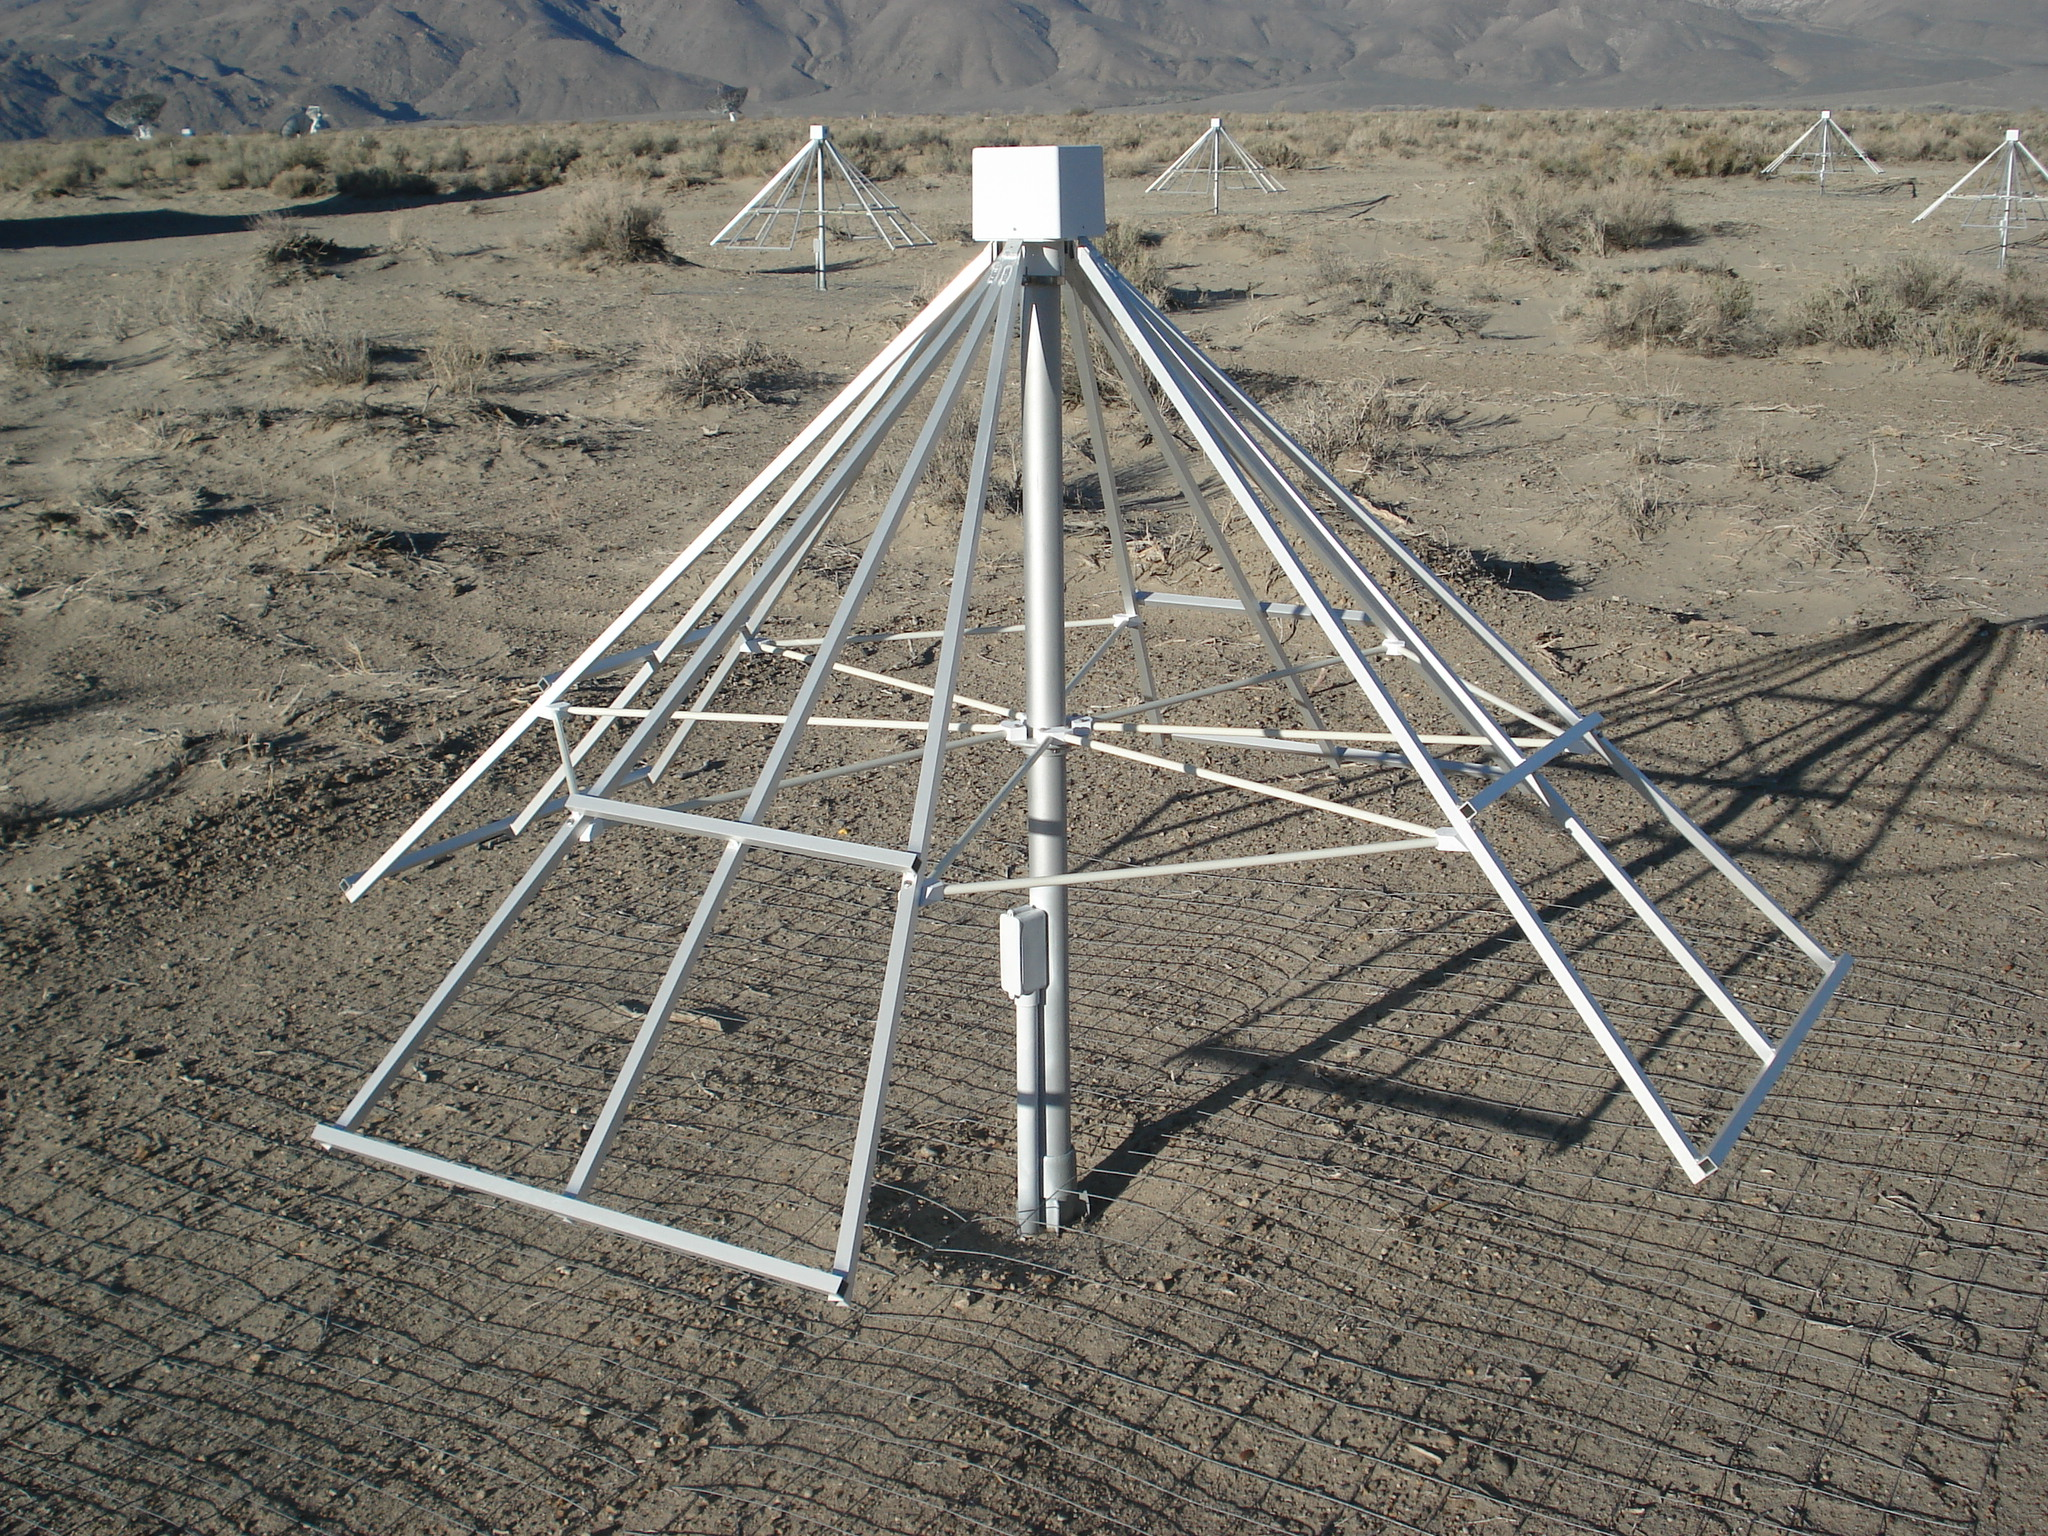
\includegraphics[height=\paperheight]{figures/antenna-picture}}
    \begin{frame}\end{frame}

    \usebackgroundtemplate{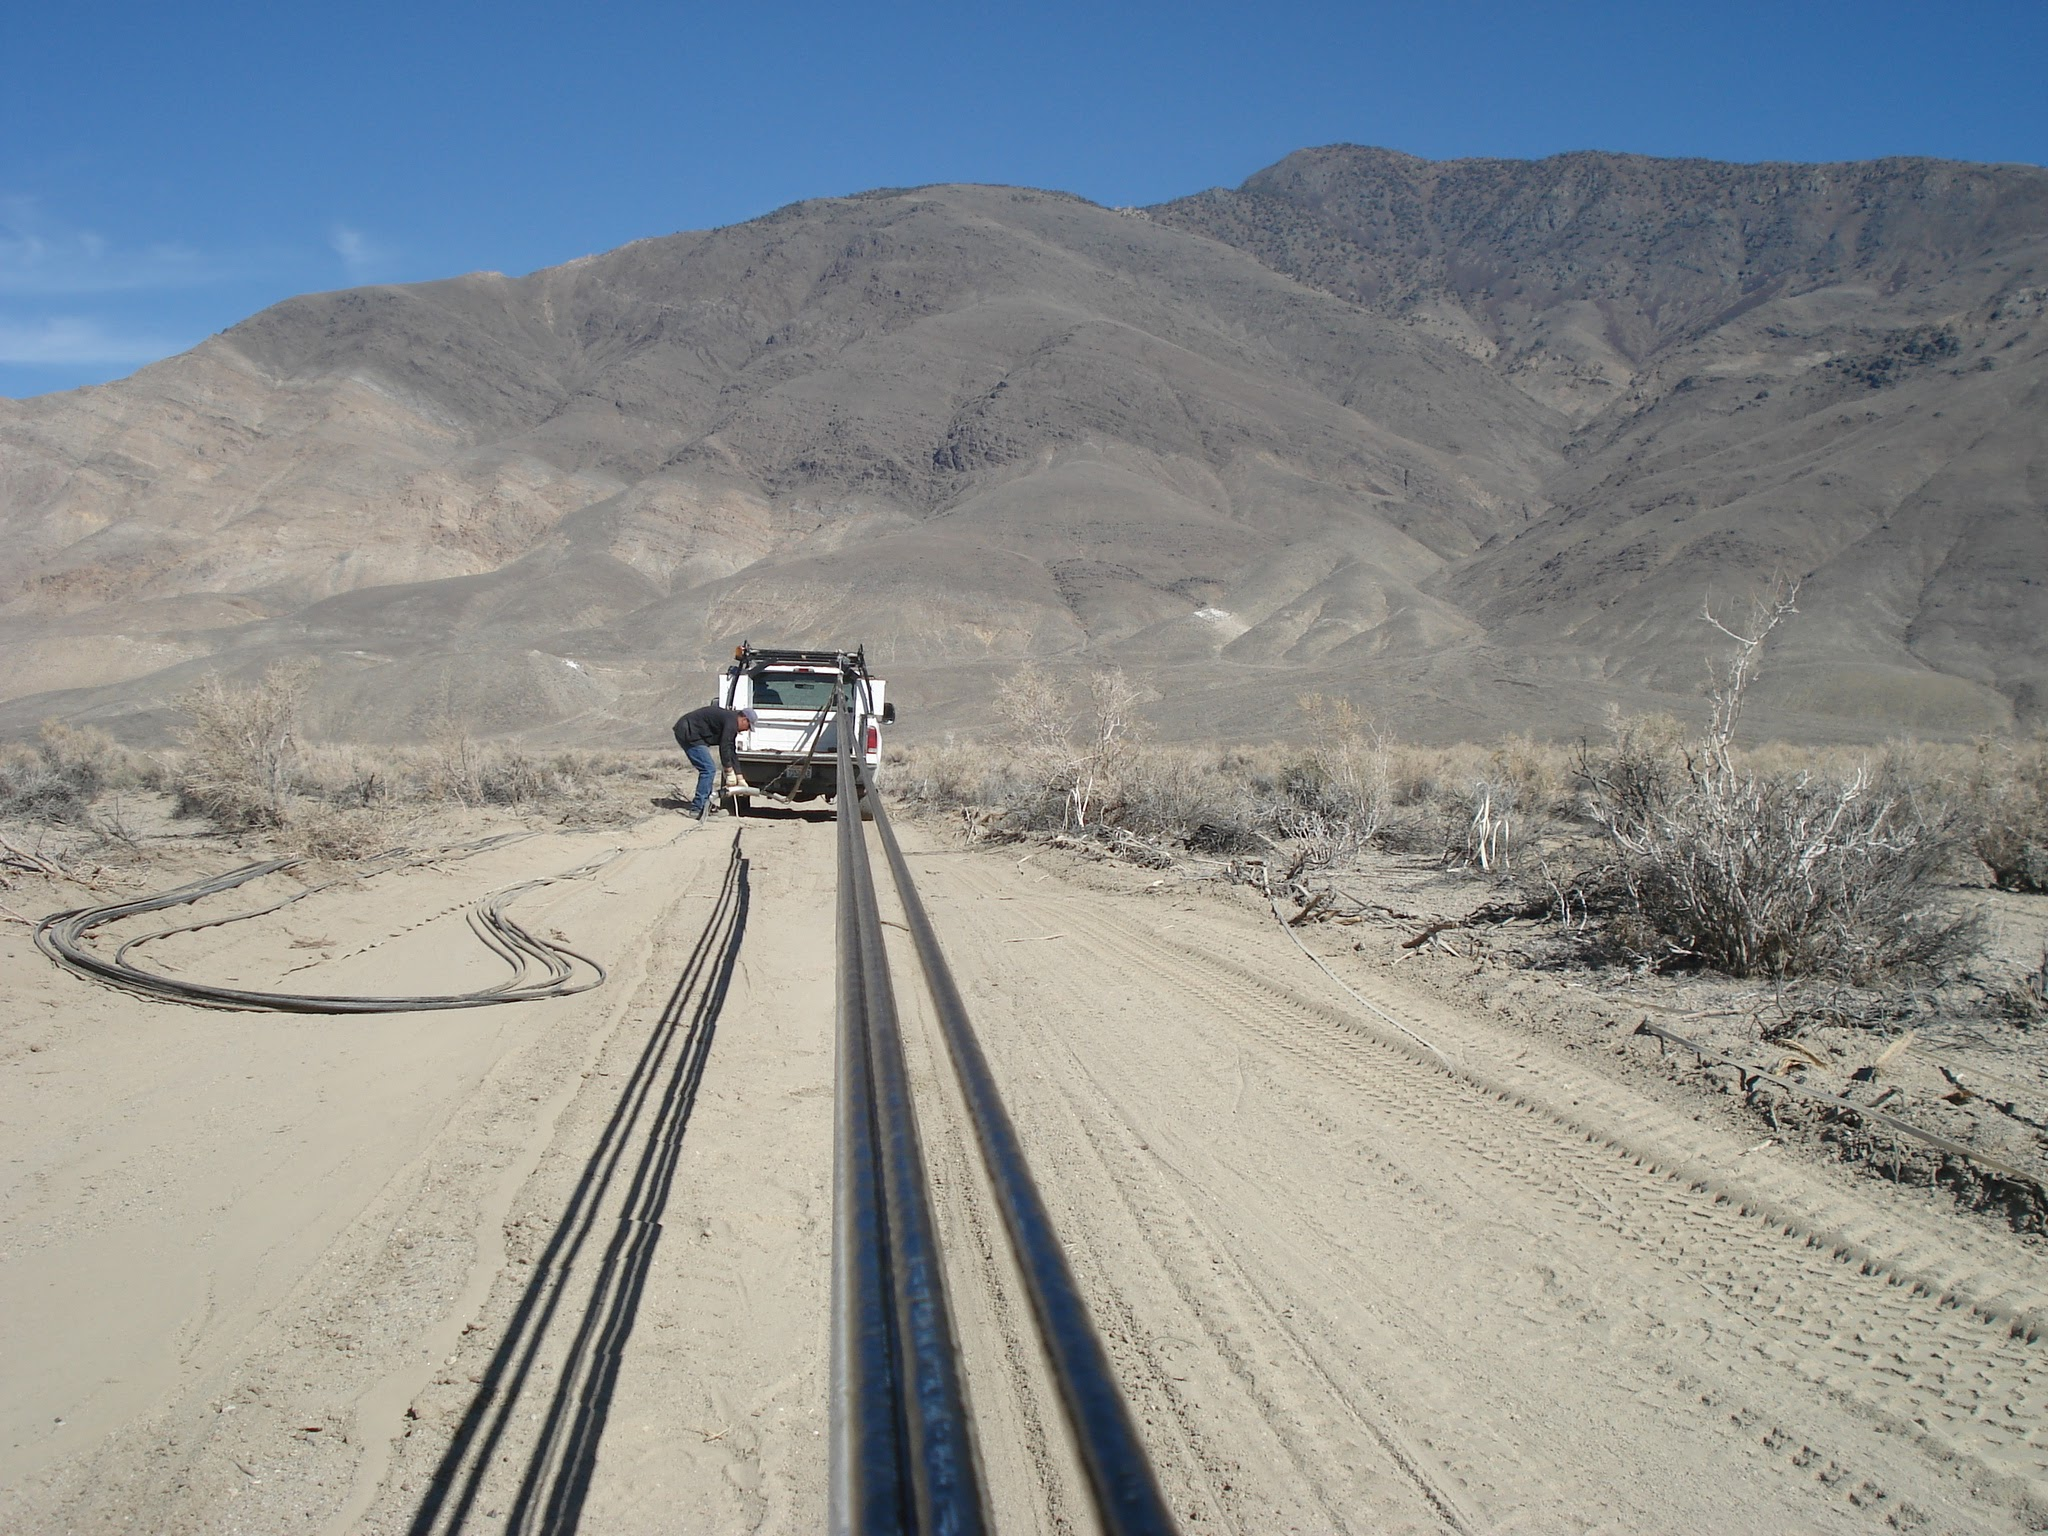
\includegraphics[height=\paperheight]{figures/lots-of-cables-1}}
    \begin{frame}\end{frame}

    \usebackgroundtemplate{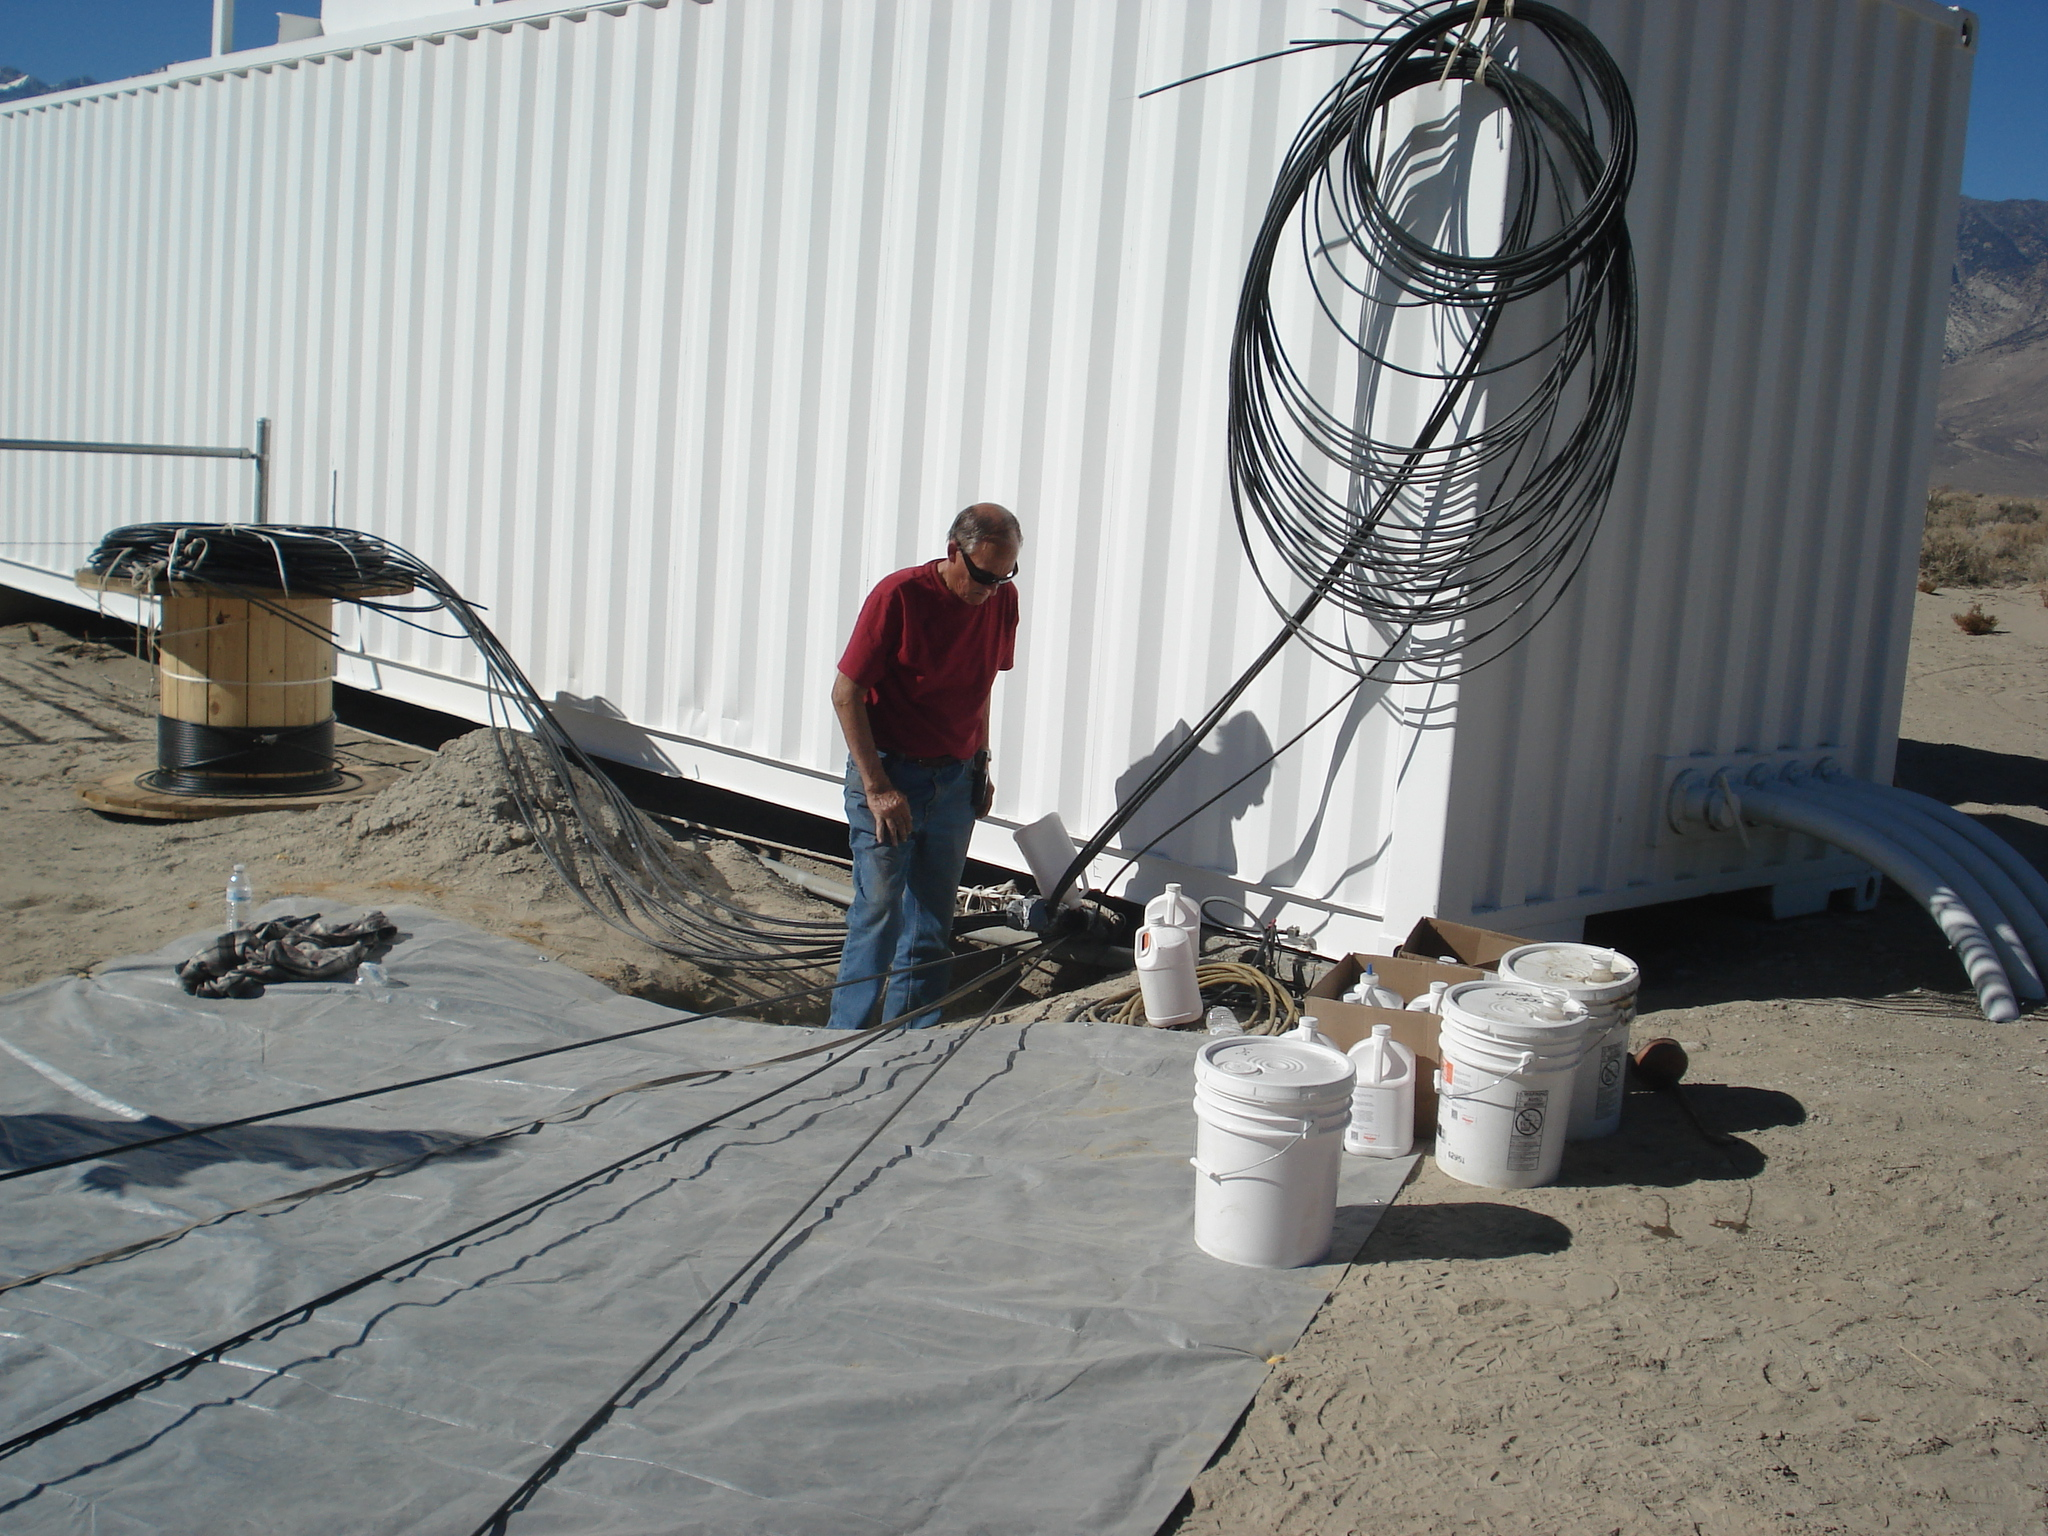
\includegraphics[height=\paperheight]{figures/ron-at-electronics-shelter}}
    \begin{frame}\end{frame}

    \usebackgroundtemplate{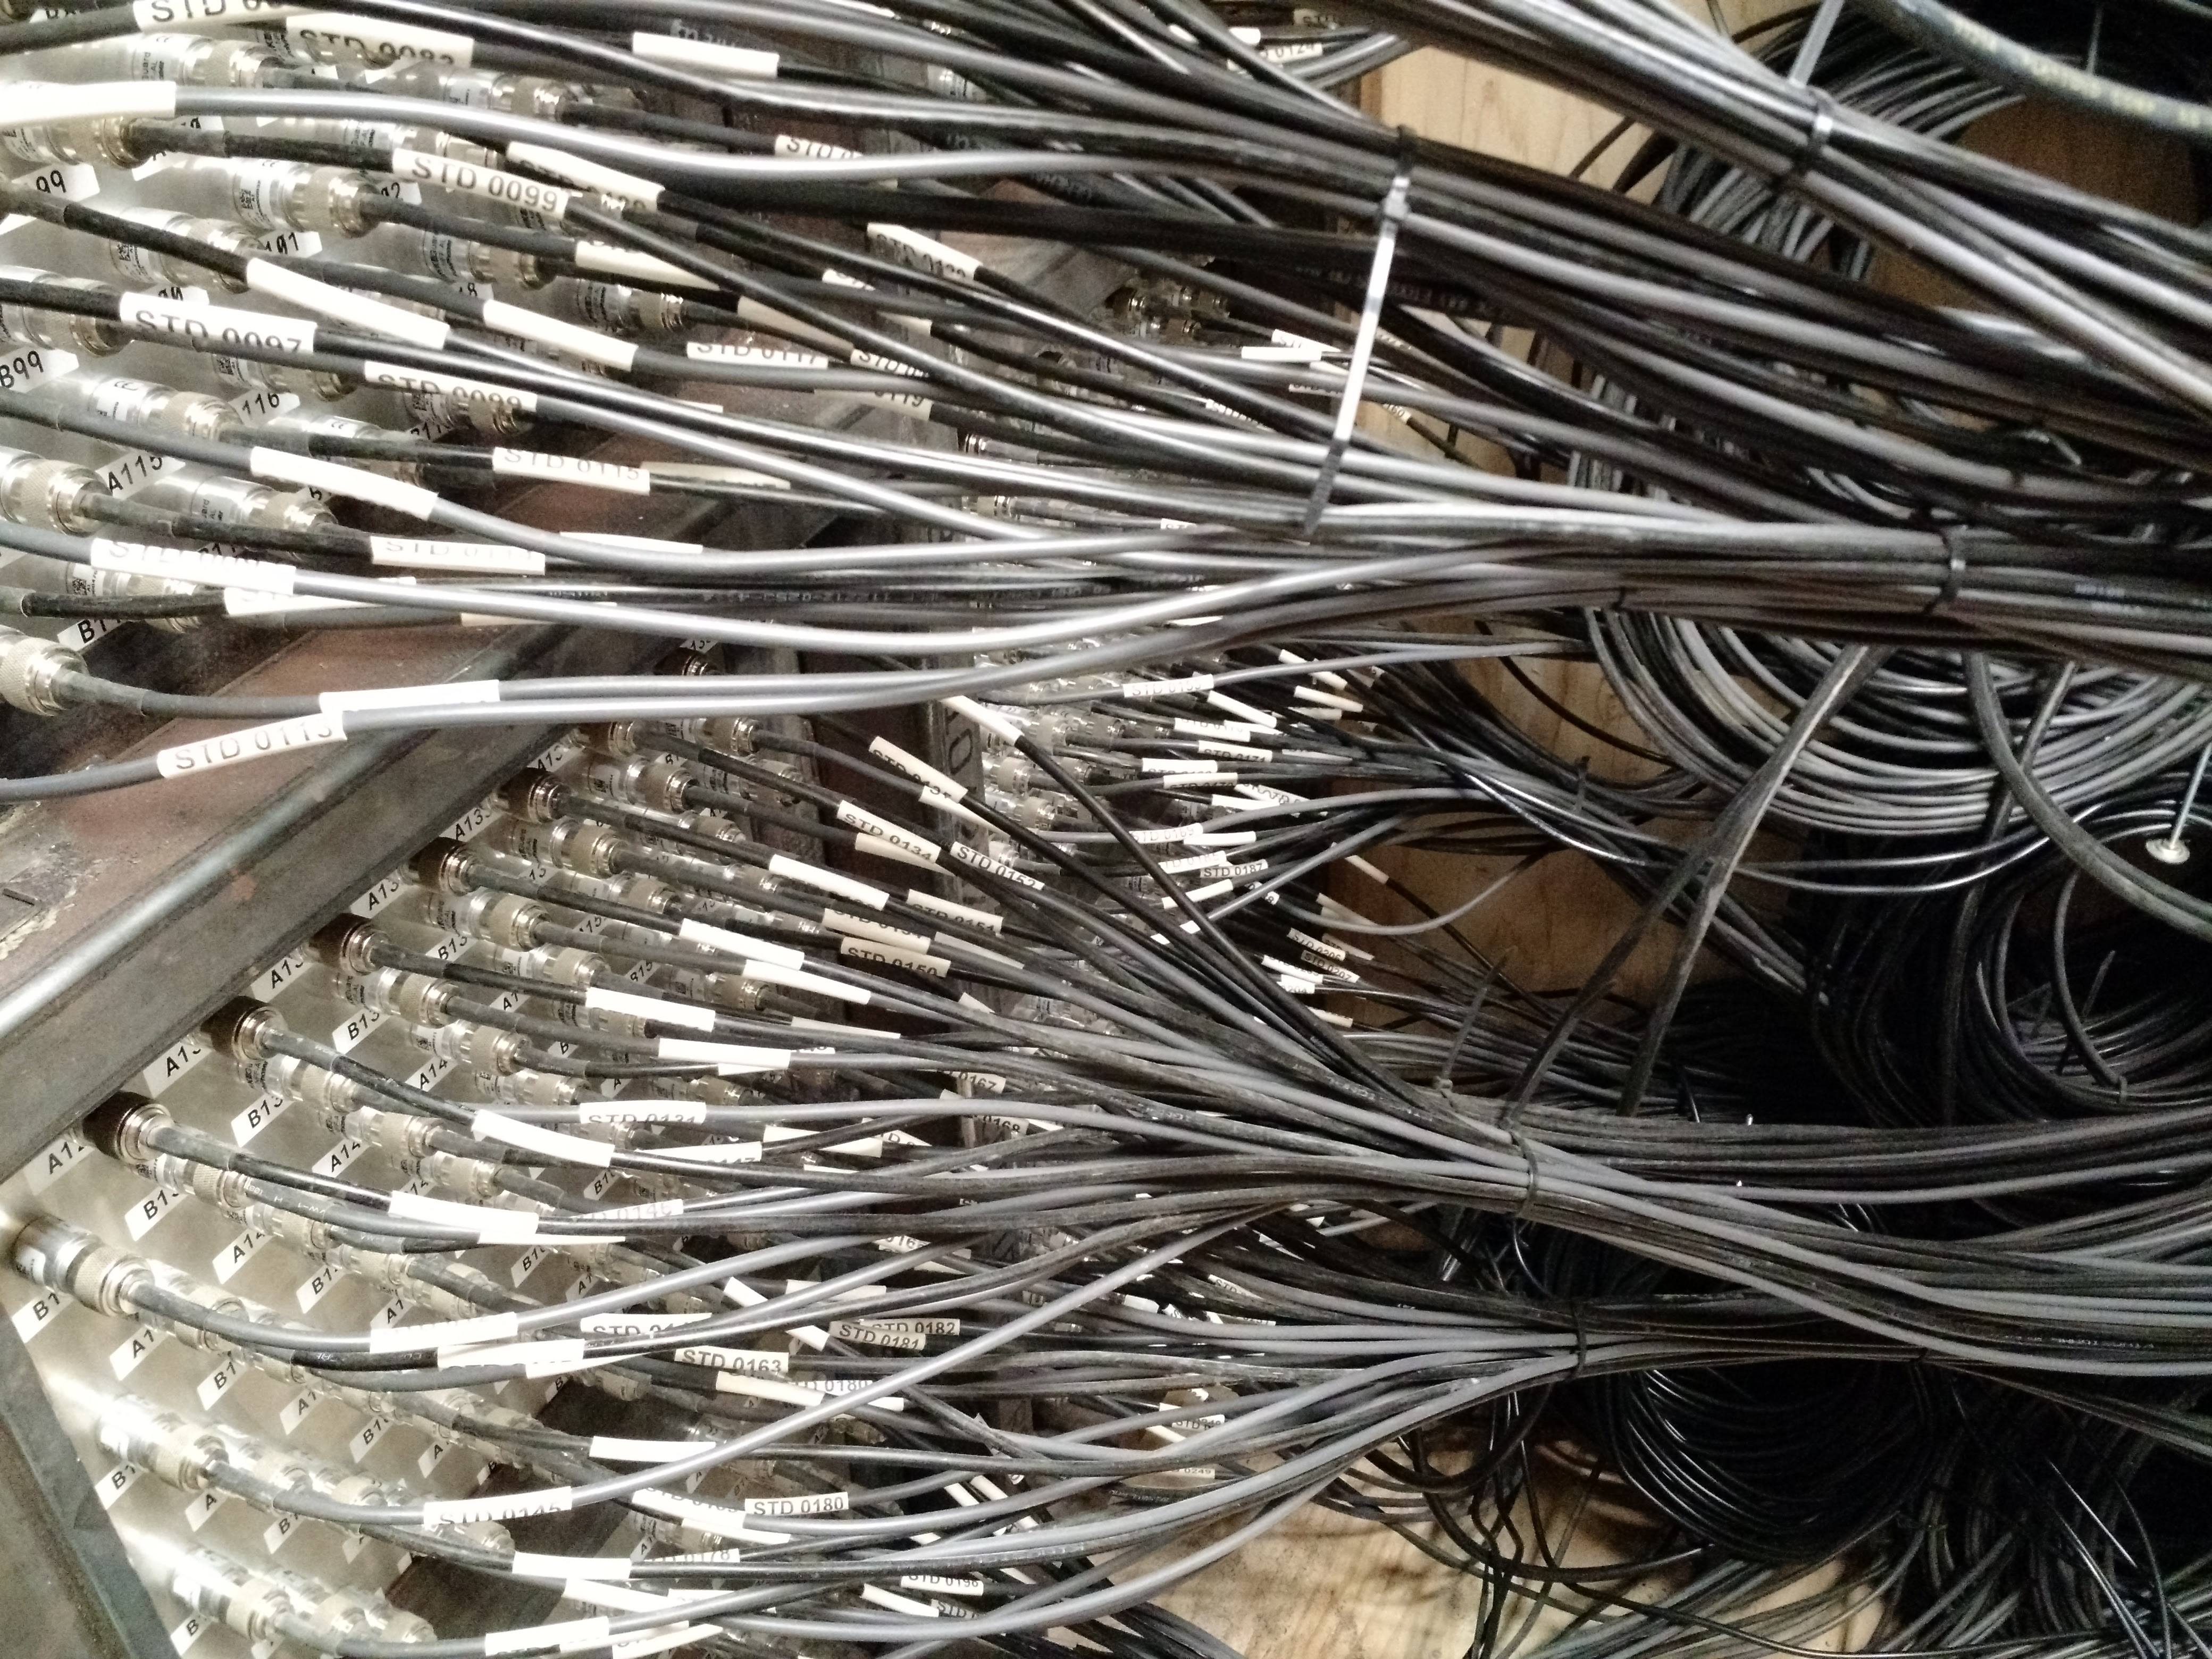
\includegraphics[height=\paperheight]{figures/lots-of-cables-2}}
    \begin{frame}\end{frame}

    \usebackgroundtemplate{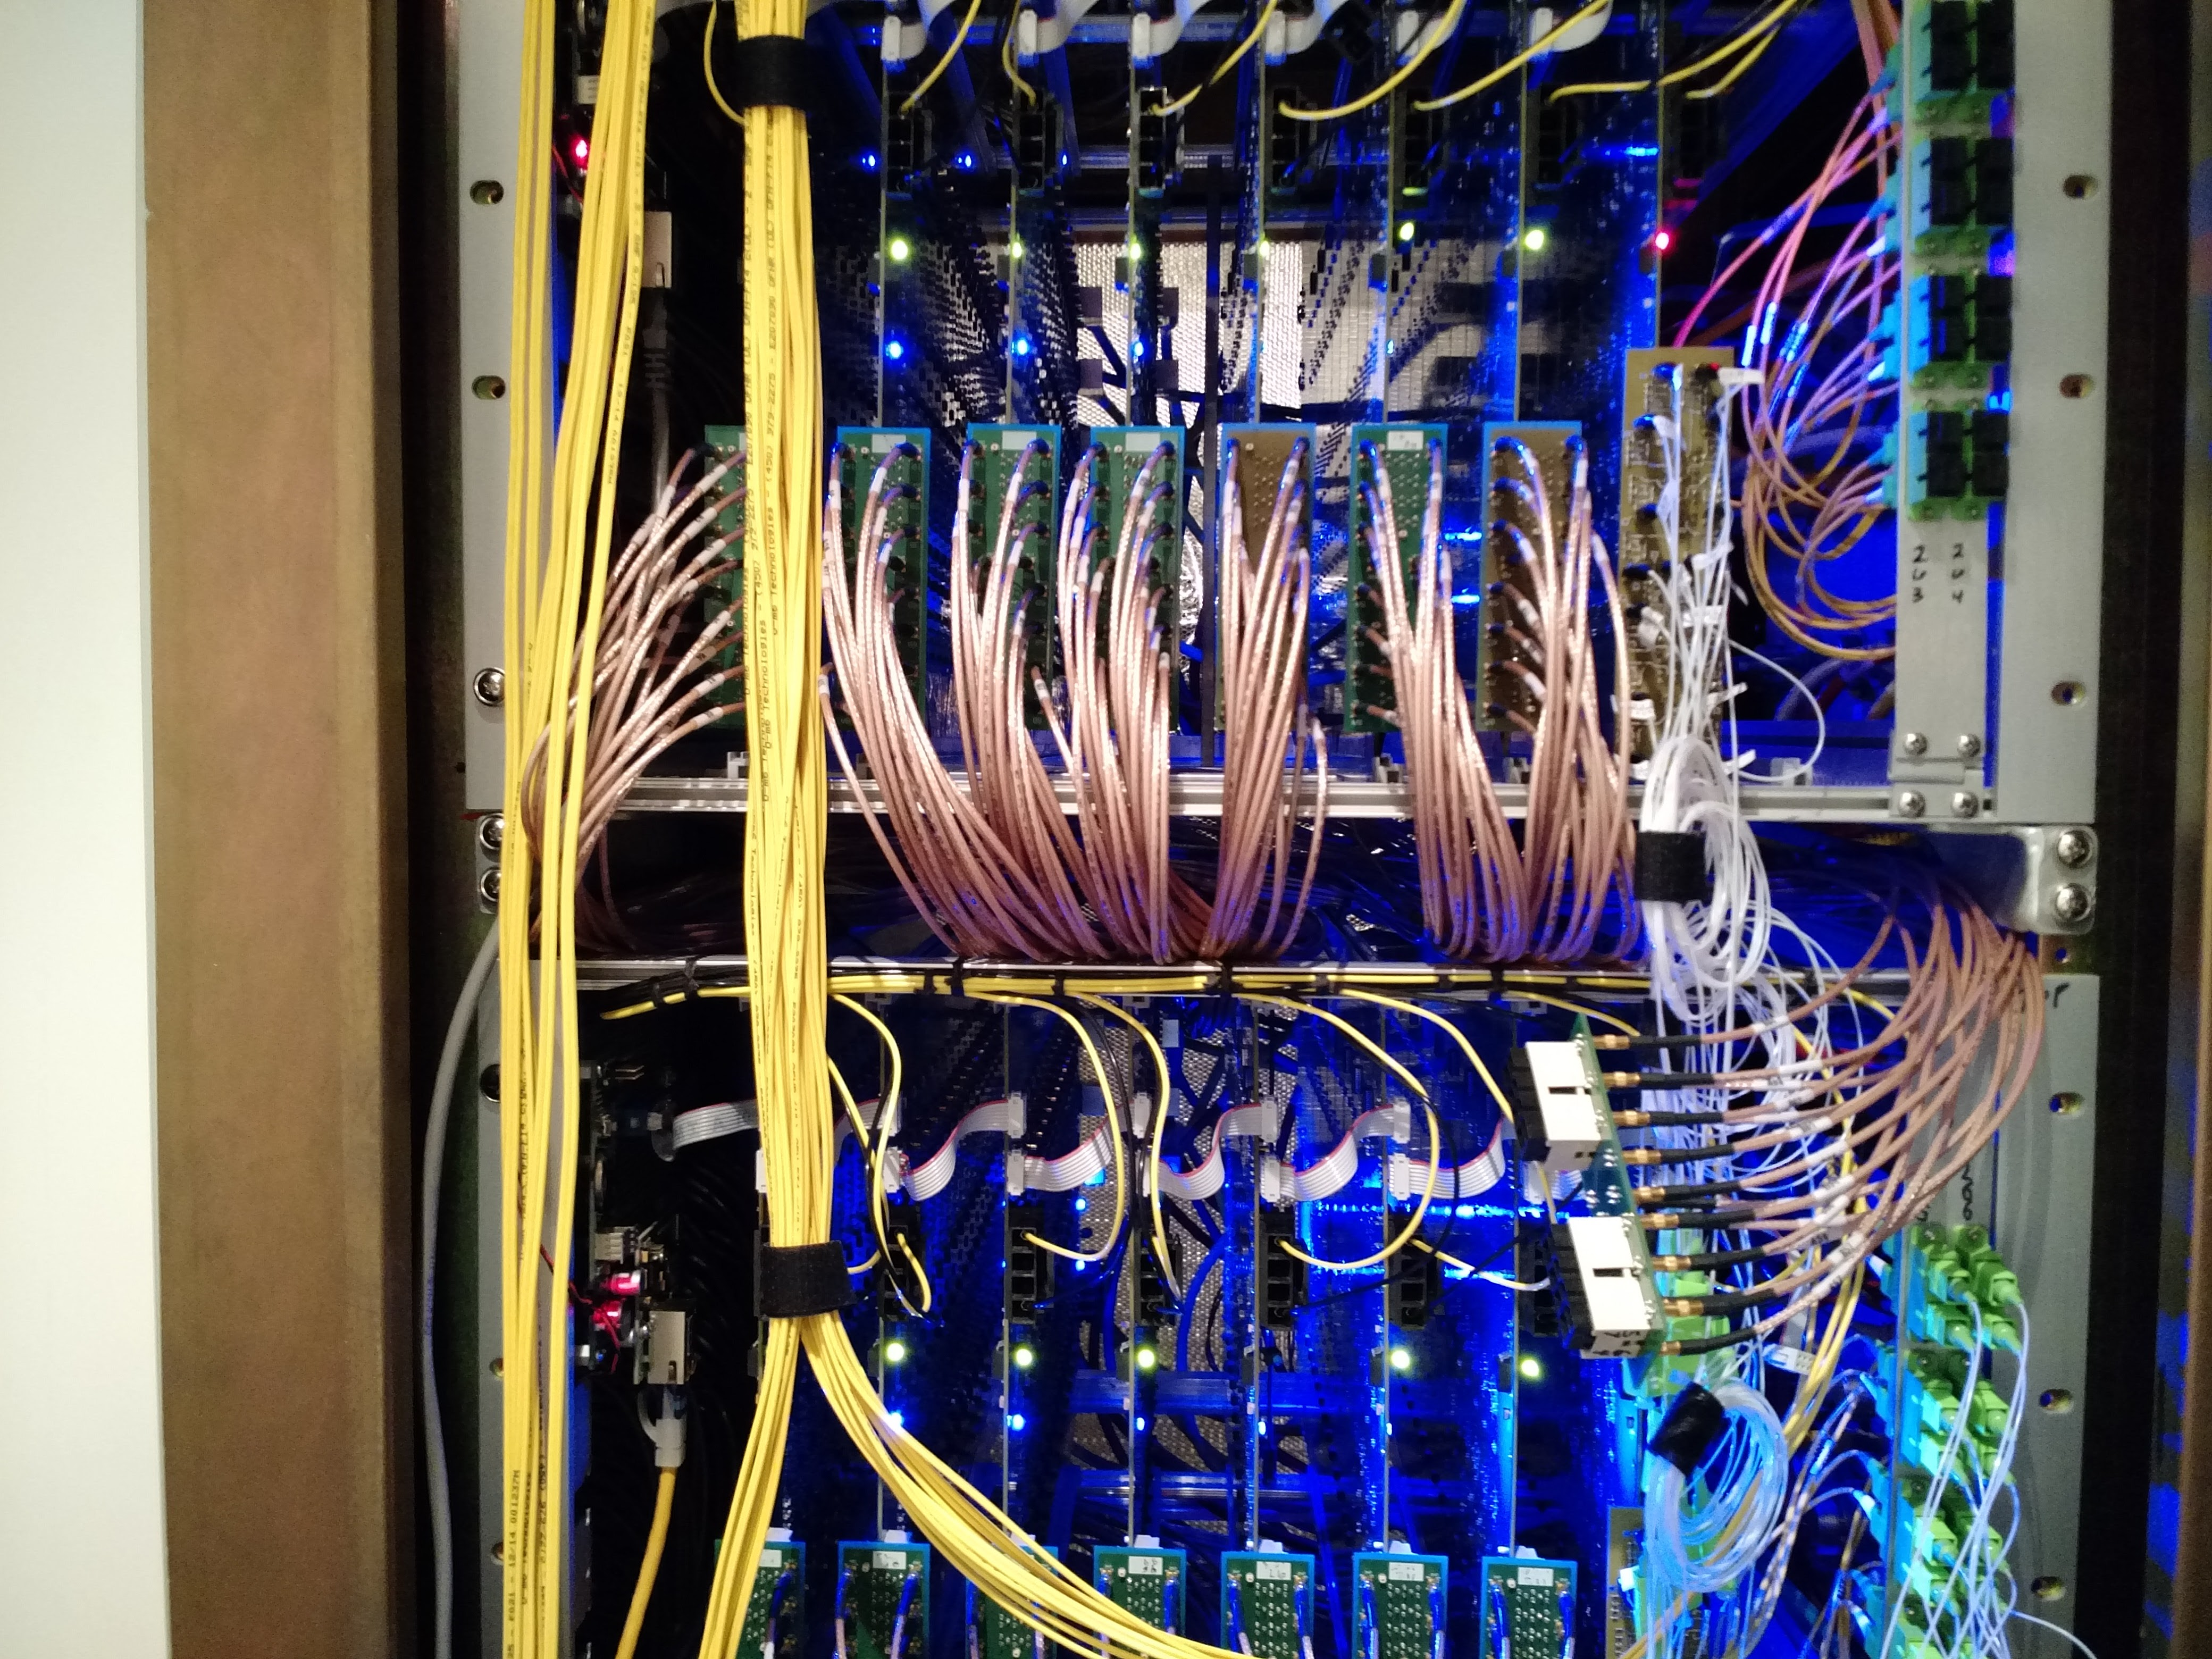
\includegraphics[height=\paperheight]{figures/asp-rack}}
    \begin{frame}\end{frame}

    \usebackgroundtemplate{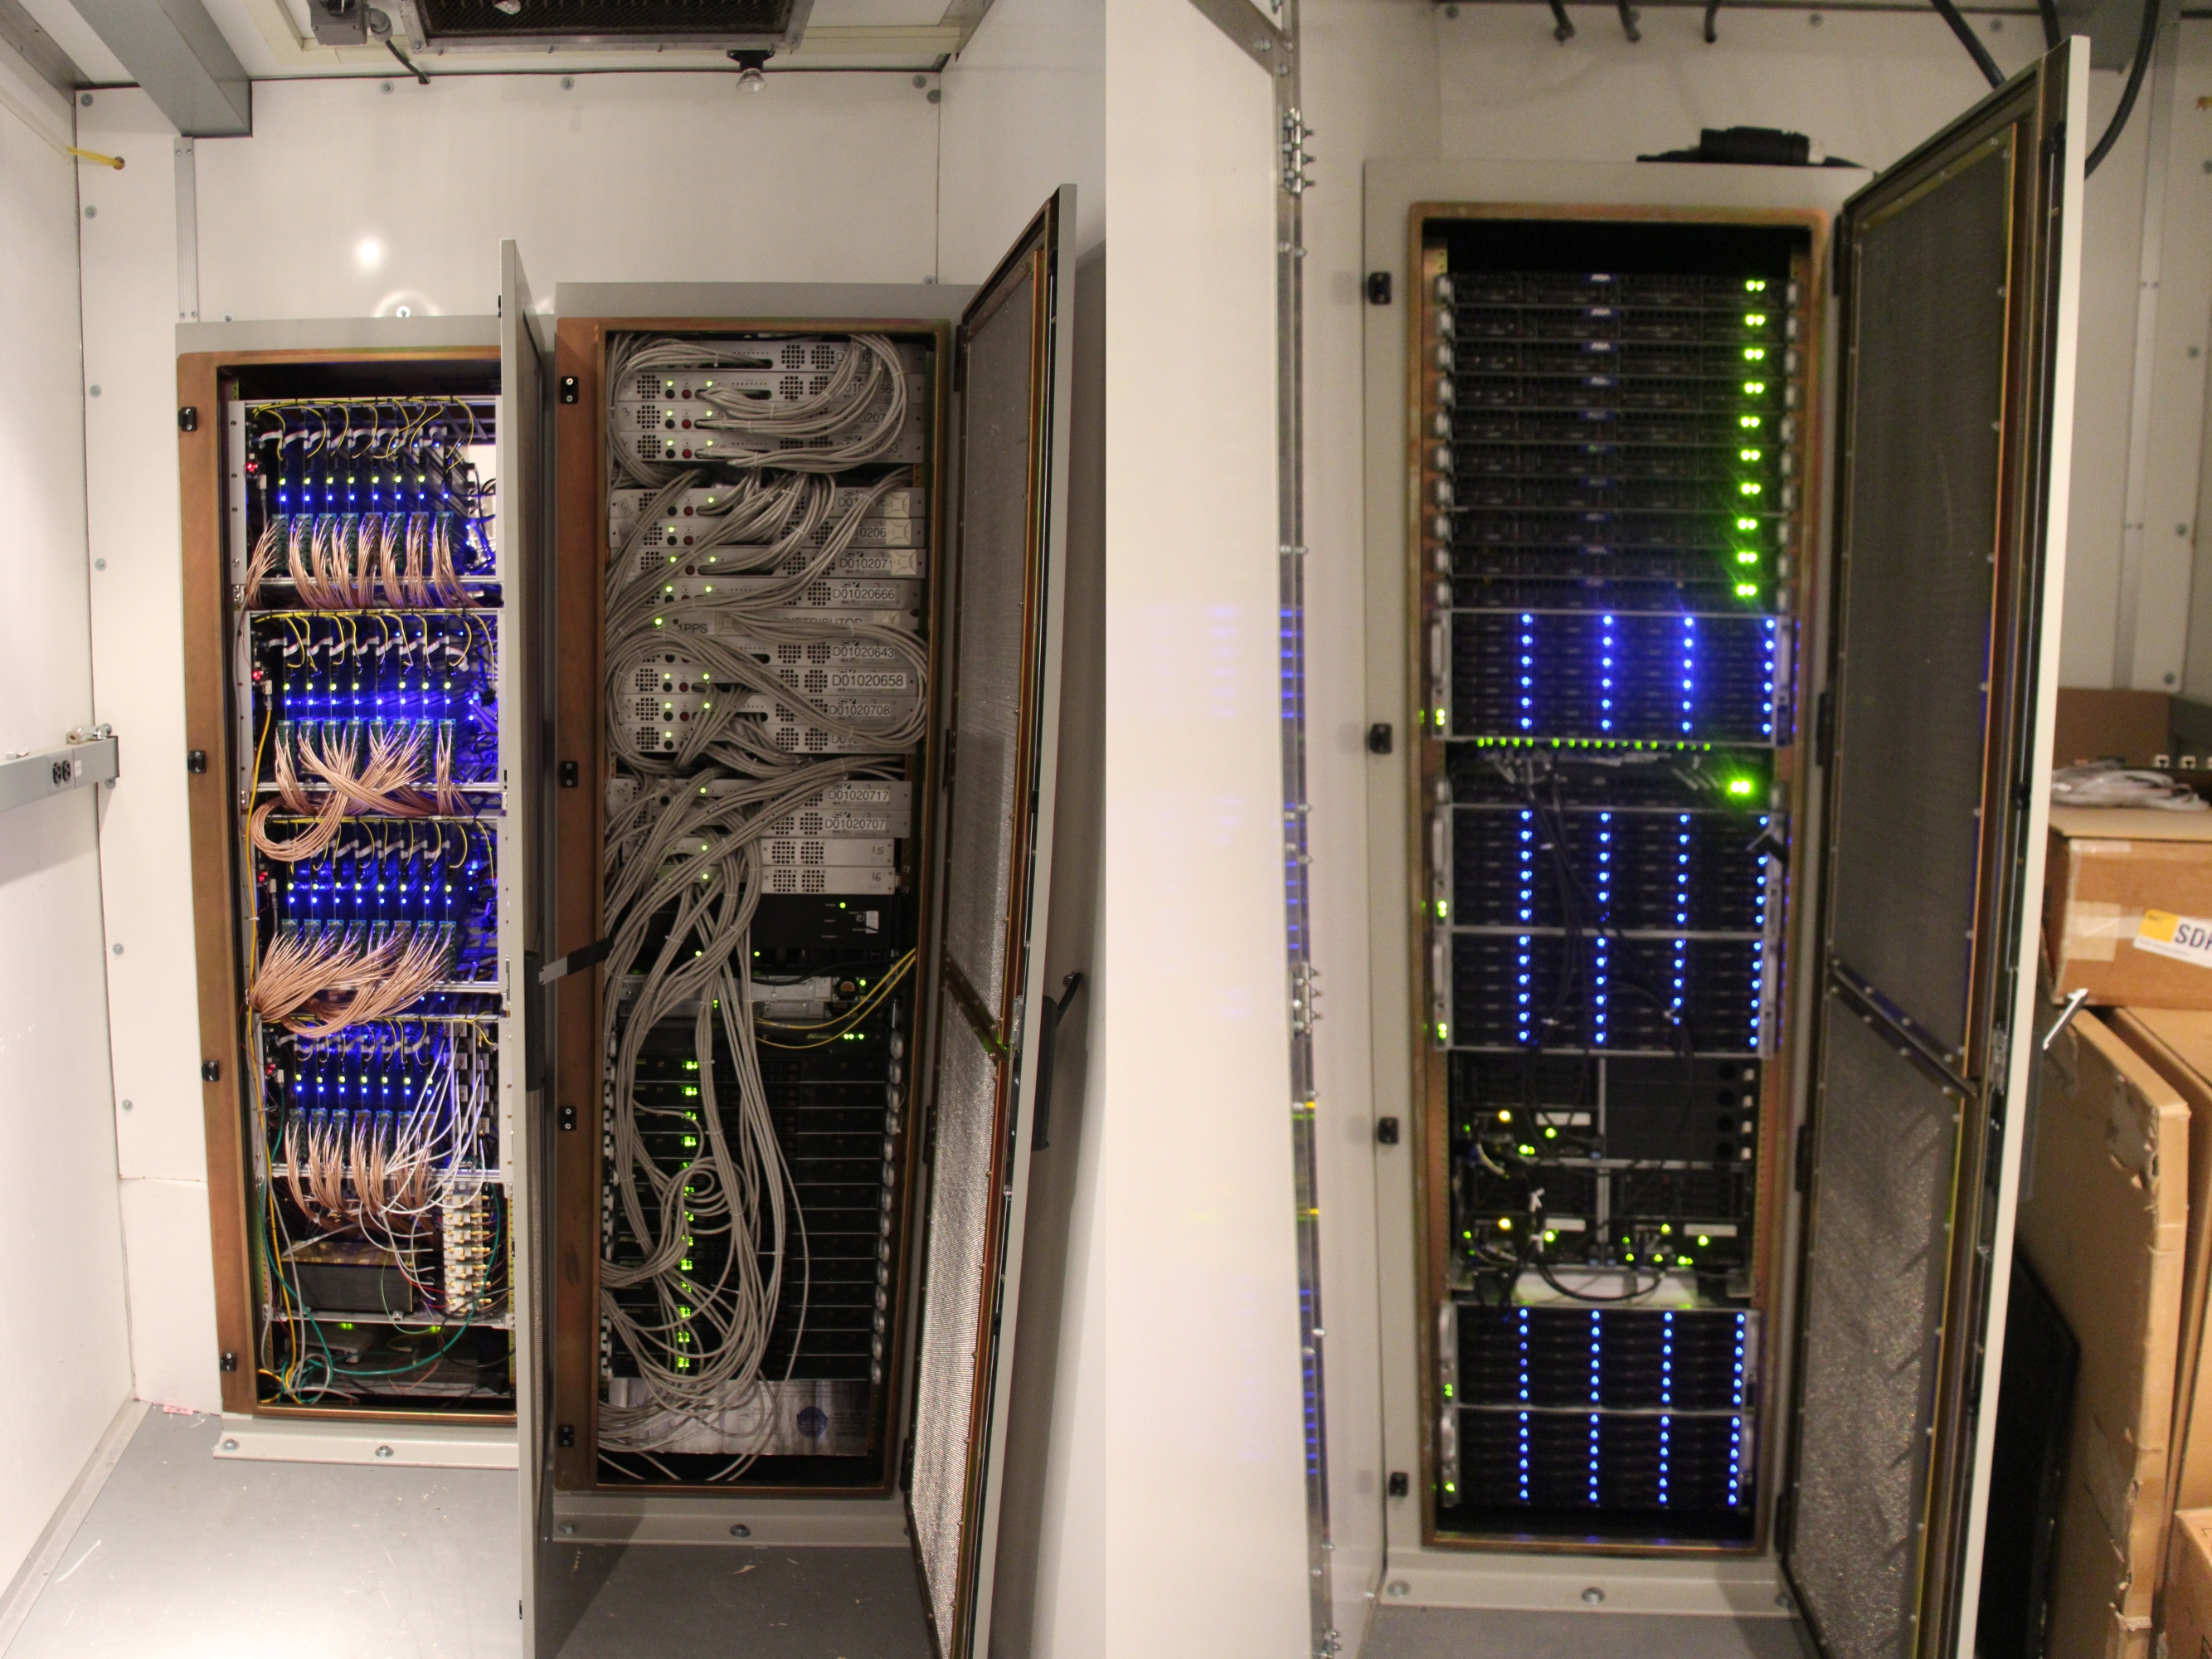
\includegraphics[height=\paperheight]{figures/all-the-computers}}
    \begin{frame}\end{frame}
}

{
    \usebackgroundtemplate{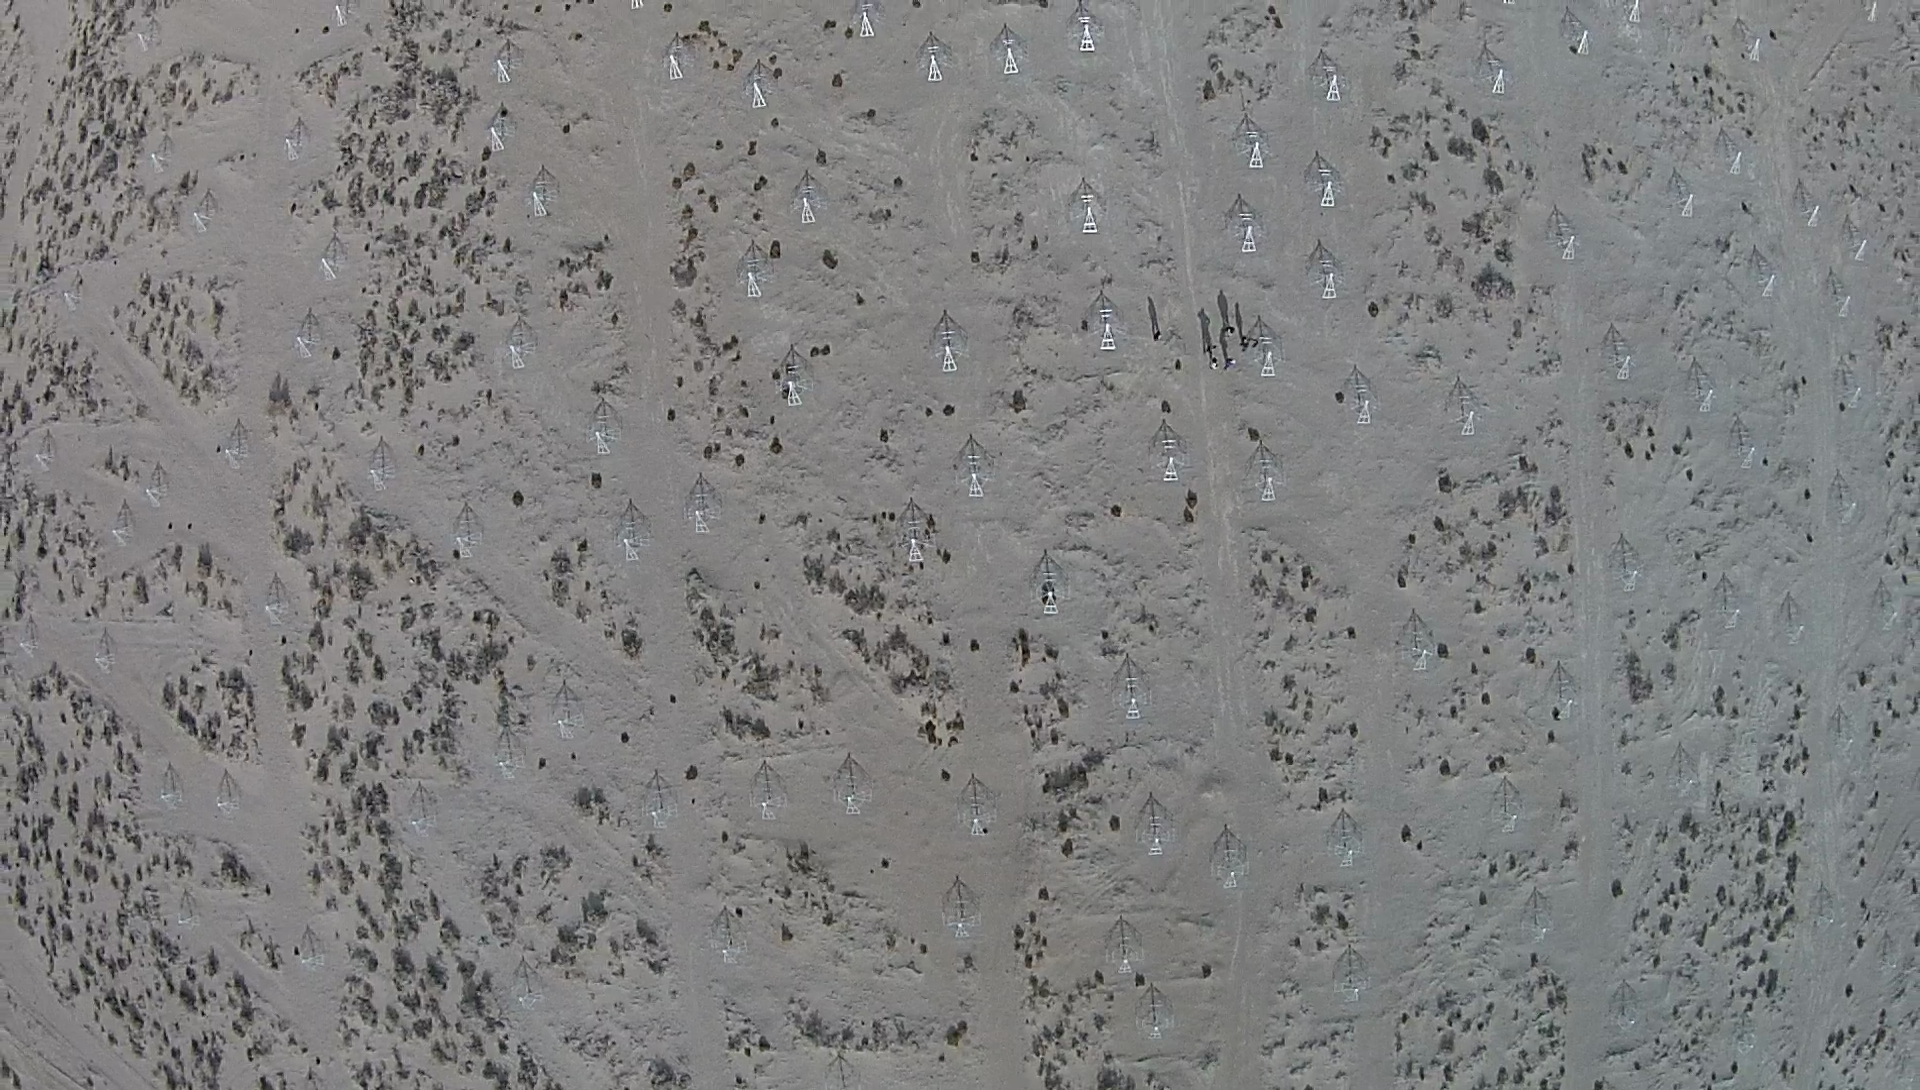
\includegraphics[height=\paperheight]{movies/ovro-lwa-drone-footage}}
    \begin{frame}
        \begin{tikzpicture}[overlay, remember picture]
            \node[anchor=center] at (current page.center) {
                \href{run:movies/ovro-lwa-drone-footage.mp4} {
                    
\includegraphics[width=30pt]{movies/play-button}
                }
            };
        \end{tikzpicture}
    \end{frame}
}

\begin{frame}
    \begin{center}
        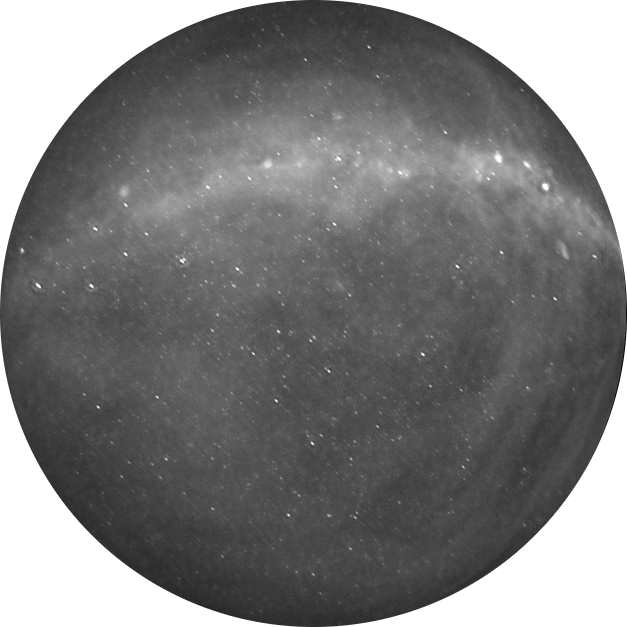
\includegraphics[height=0.95\textheight]{movies/marin-sGRB-fullband}
    \end{center}
    \begin{tikzpicture}[overlay, remember picture]
        \node[anchor=center] at (current page.center) {
            \href{run:movies/marin-sGRG-fullband.mp4} {
                
\includegraphics[width=30pt]{movies/play-button}
            }
        };
    \end{tikzpicture}
\end{frame}

{
    \usebackgroundtemplate{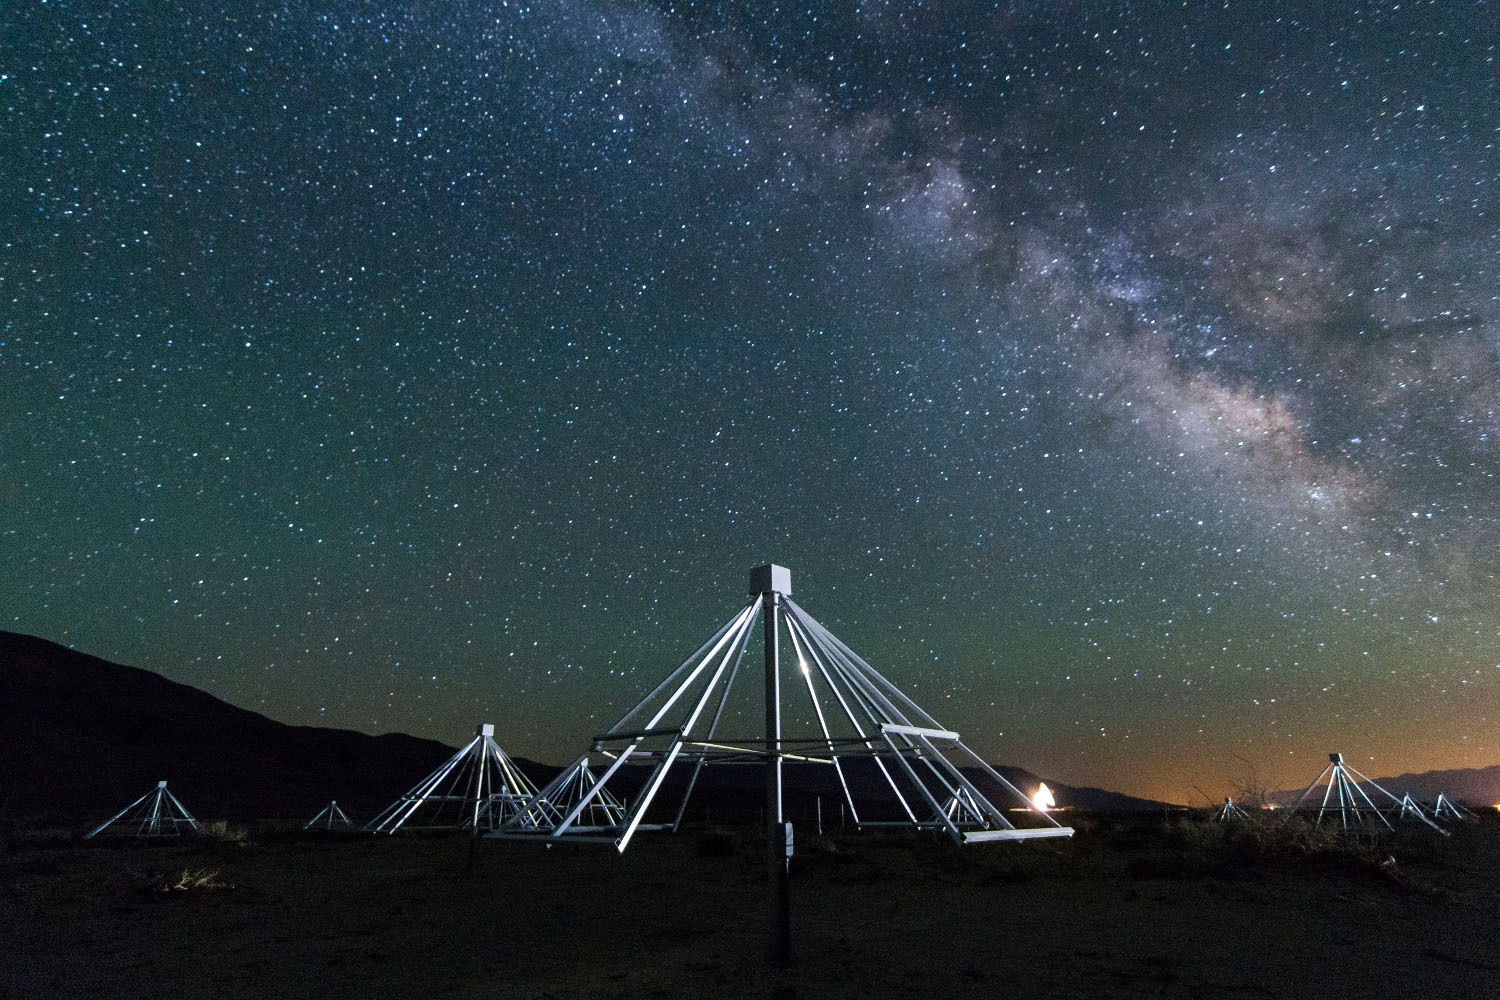
\includegraphics[height=\paperheight]{figures/lwa-night}}
    \begin{frame}[t]{The OVRO-LWA}
        \vskip -5pt
        \small
        \begin{tabular}{rl}
            \textbf{Number of Antennas} & 288 (256 correlated) \\
            \textbf{Core Diameter} & 200\,m \\
            \textbf{Maximum Baseline} & 1.5\,km \\
            \textbf{Resolution} & 10--20\,arcmin \\
            \textbf{Frequency Range} & 27--85\,MHz \\
            \textbf{Frequency Resolution} & 24\,kHz \\
            \textbf{Field of View} & Entire hemisphere \\
            \textbf{Integration Time (this work)} & 28\,hr \\
        \end{tabular}
    \end{frame}
}

\begin{frame}{Commissioning Challenges}
    \begin{itemize}[label=\textbullet]
        \item Gain calibration
        \item Gain fluctuations
        \item {\color{yellow} Direction-dependent calibration}
        \item Antenna positions
        \item Frequency labels
        \item RFI localization
        \item Common-mode RFI
        \item Primary beam mapping
    \end{itemize}
\end{frame}

\begin{frame}{Adaptive Optics}
    \begin{overprint}
        \onslide<1>
        \begin{center}
            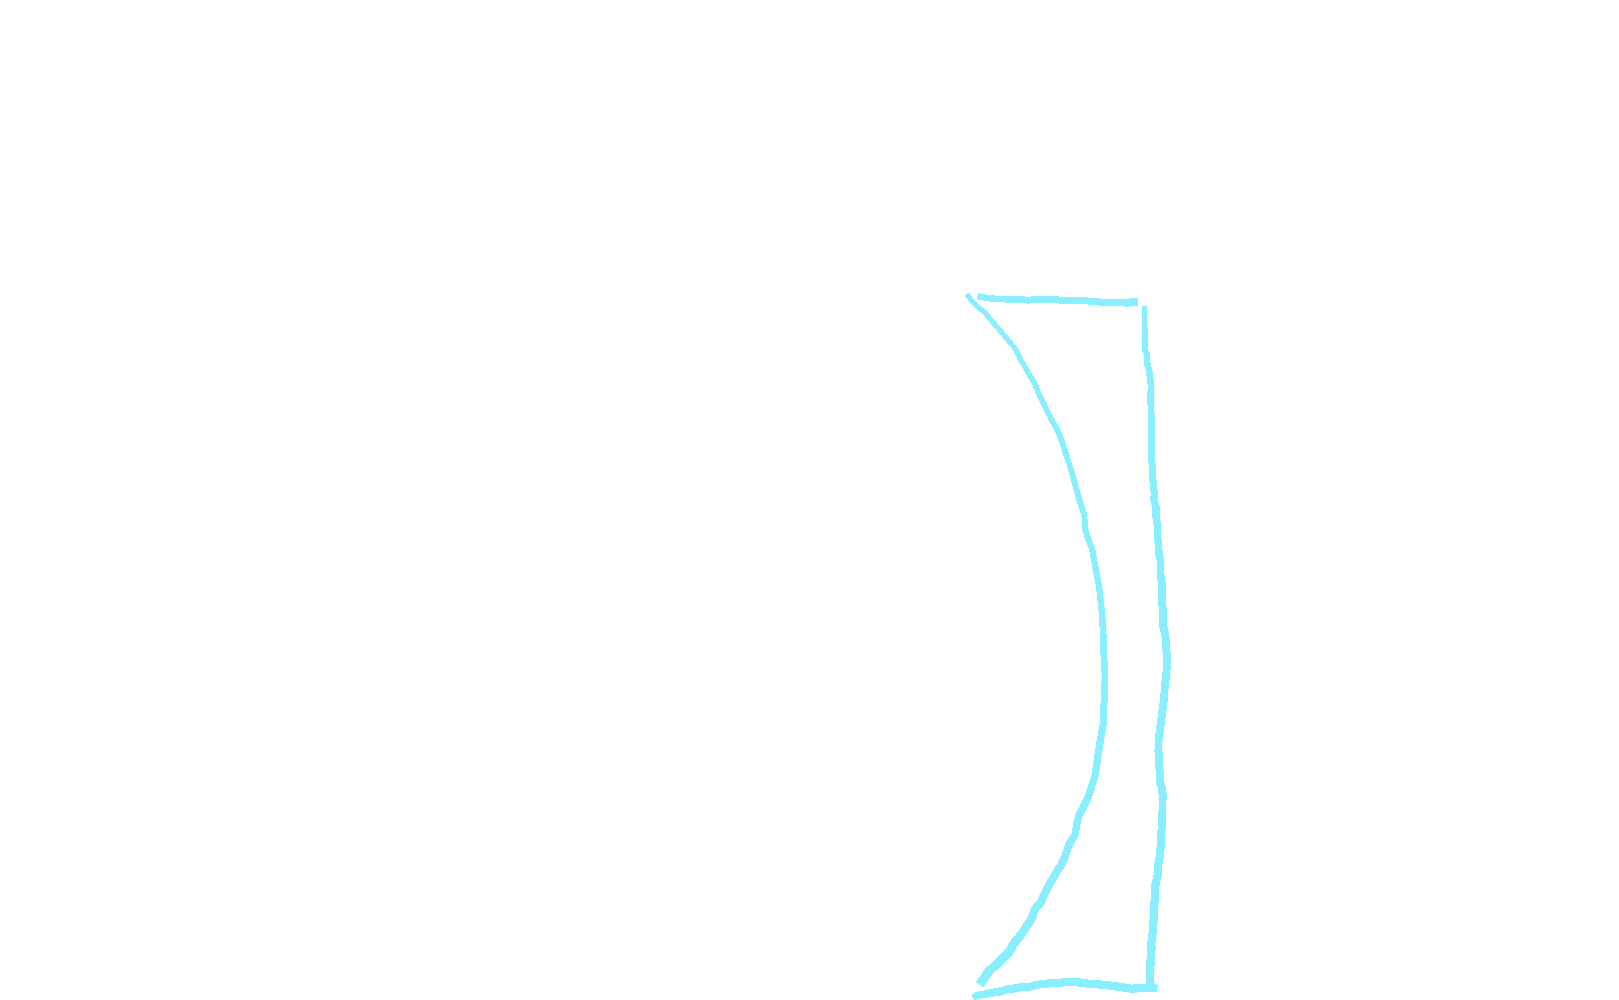
\includegraphics[width=0.8\textwidth]{figures/ao-1}
        \end{center}
        \onslide<2>
        \begin{center}
            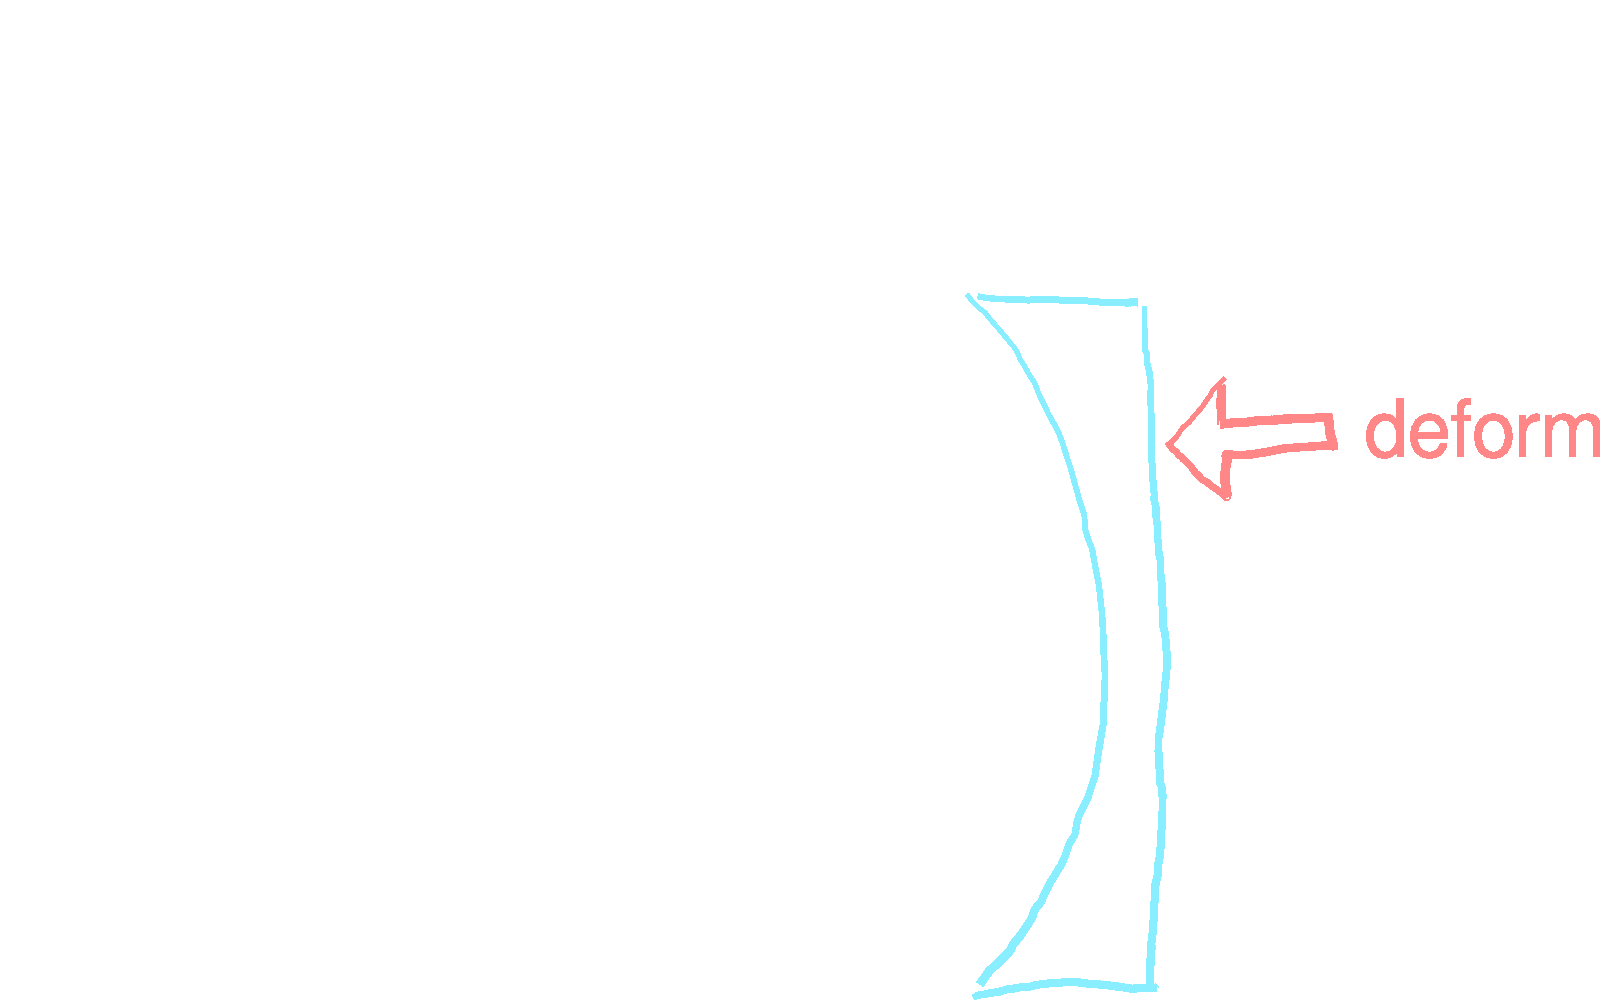
\includegraphics[width=0.8\textwidth]{figures/ao-2}
        \end{center}
        \onslide<3>
        \begin{center}
            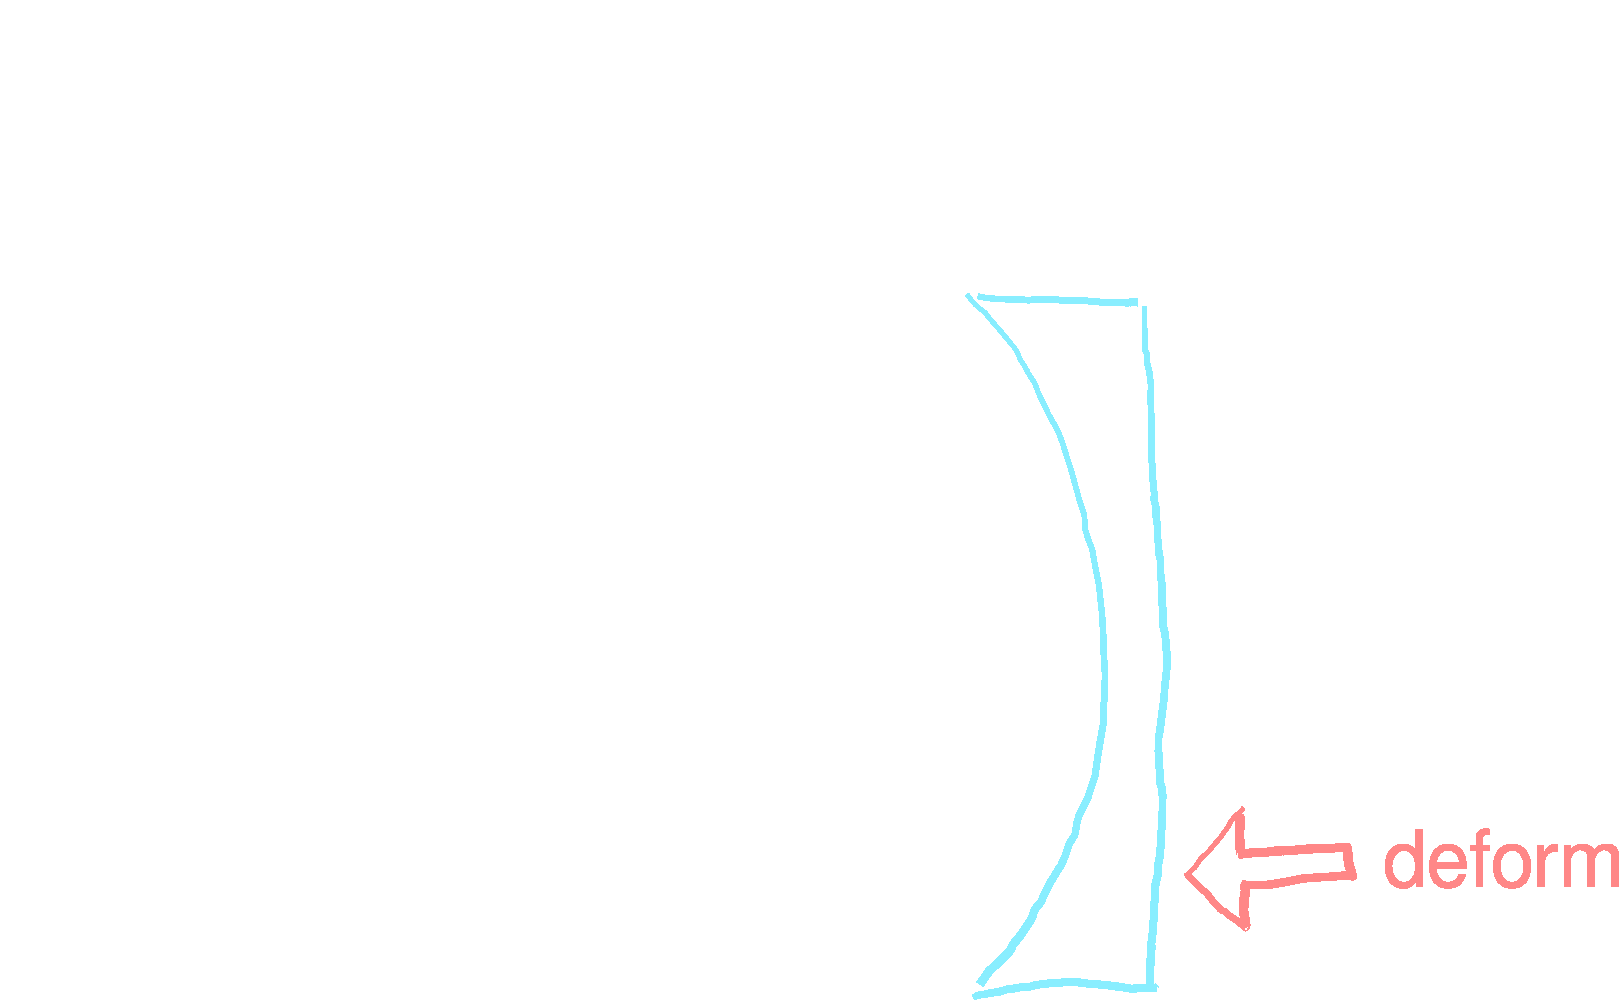
\includegraphics[width=0.8\textwidth]{figures/ao-3}
        \end{center}
    \end{overprint}
\end{frame}

\begin{frame}{Direction-Dependent Calibration}
    \begin{overprint}
        \onslide<1>
        \begin{center}
            Image of Cas A prior to removal \\
            \vskip 10pt
            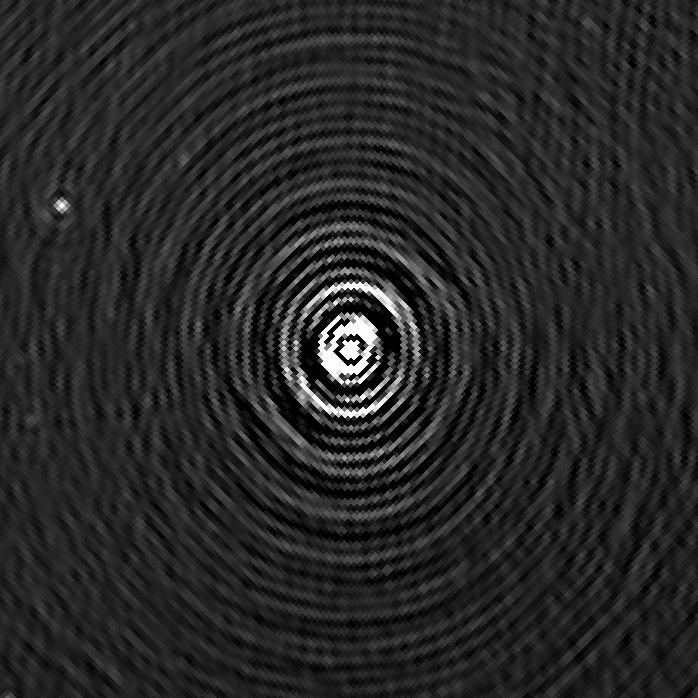
\includegraphics[height=0.6\textheight]{figures/cas-a-no-removal}
        \end{center}
        \onslide<2>
        \begin{center}
            ... after removing \textbf{without} direction dependent calibration \\
            \vskip 10pt
            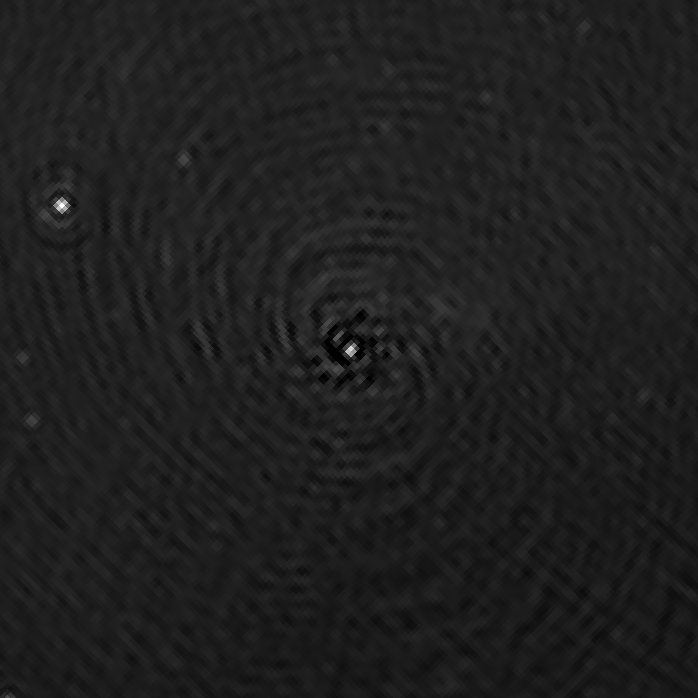
\includegraphics[height=0.6\textheight]{figures/cas-a-subtraction}
        \end{center}
        \onslide<3>
        \begin{center}
            ... after removing \textbf{with} direction dependent calibration \\
            \vskip 10pt
            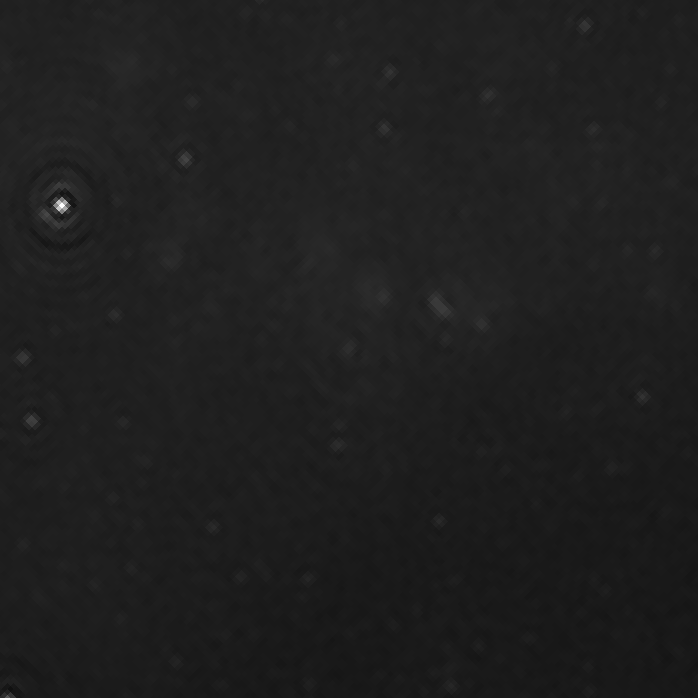
\includegraphics[height=0.6\textheight]{figures/cas-a-peeling}
        \end{center}
    \end{overprint}
\end{frame}

\begin{frame}
    \begin{tabularx}{\textwidth}{X|X}
        \begin{minipage}[t]{\linewidth}
            \hspace{0.5em}\Large \textbf{The Cosmic Dawn}
            \footnotesize
            \begin{itemize}[label=\textbullet]
                \item First generation of stars
                \item Formation and feedback
                \item Heating of the IGM
                \item Early X-ray sources
            \end{itemize}
        \end{minipage}\vskip 0.5em &
        \begin{minipage}[t]{\linewidth}
            \hspace{0.5em}\Large \textbf{Transients}
            \footnotesize
            \begin{itemize}[label=\textbullet]
                \item Stellar flares
                \item Extrasolar planets
                \item SWIFT and LIGO follow-up
                \item \color{yellow} See Anderson thesis
            \end{itemize}
        \end{minipage} \vskip 0.5em \\ \hline
        \vskip 0.5em \begin{minipage}[t]{\linewidth}
            \hspace{0.5em}\Large \textbf{Space Weather}
            \footnotesize
            \begin{itemize}[label=\textbullet]
                \item Solar flares
                \item Jovian flares
            \end{itemize}
        \end{minipage} &
        \vskip 0.5em \begin{minipage}[t]{\linewidth}
            \hspace{0.5em}\Large \textbf{Cosmic Rays}
            \footnotesize
            \begin{itemize}[label=\textbullet]
                \item Real-time detection
                \item \color{yellow} See Monroe thesis
            \end{itemize}
        \end{minipage}
    \end{tabularx}
\end{frame}

%%%%%%%%%%%%%%%%%%%%%%%%%%%%%%%%%%%%%%%%%%%%%%%%%%%%%%%%%%%%%%%%%%%%%%%%%%%%%%%%%%%%%%%%%%%%%%%%%%%%

\section{III. VHF Sky Maps}

{
    \usebackgroundtemplate{
\includegraphics[height=\paperheight]{figures/waves3}}
    \begin{frame}[t]

        {\large \bfseries III. New Maps of the Sky at Meter Wavelengths}
    \end{frame}
}

\begin{frame}{Imaging and Cleaning}
    \onslide<1->{\begin{dmath*}
        \textrm{visibility} = \int \big(\textrm{sky brightness}\big)
            \times \big(\textrm{beam}\big)
            \times \big(\textrm{fringe pattern}\big) \, \d\Omega  
    \end{dmath*}}
    \onslide<2->{\begin{dmath*}
        \textrm{visibility} \xrightarrow{\textrm{\small sidereal time Fourier transform}} \textrm{m-mode}
    \end{dmath*}}
    \onslide<3->{\begin{dmath*}
        \underbrace{\left(
            \begin{array}{c}
                \vdots \\
                \textrm{m-modes} \\
                \vdots \\
            \end{array}
        \right)}_{\b v}
        =
        \underbrace{\left(
            \begin{array}{ccc}
                \ddots & & \\
                       & \textrm{transfer matrix} & \\
                       & & \ddots \\
            \end{array}
        \right)}_{\b B}
        \underbrace{\left(
            \begin{array}{c}
                \vdots \\
                a_{lm} \\
                \vdots \\
            \end{array}
        \right)}_{\b a}
    \end{dmath*}}
    \begin{center}
        \tiny{Shaw et al. (2014, 2015)}
    \end{center}
    \onslide<4->{\begin{dmath*}
        \b{\hat a} = \argmin \left\{ \|\b v - \b B\b a\|^2 + \varepsilon\|\b a\|^2 \right\} \nolinebreak
            = (\b B^* \b B + \varepsilon \b I)^{-1} \b B^* \b v
    \end{dmath*}
    \begin{center}
        \tiny{Eastwood et al. (2018)}
    \end{center}}
\end{frame}

{
    \usebackgroundtemplate{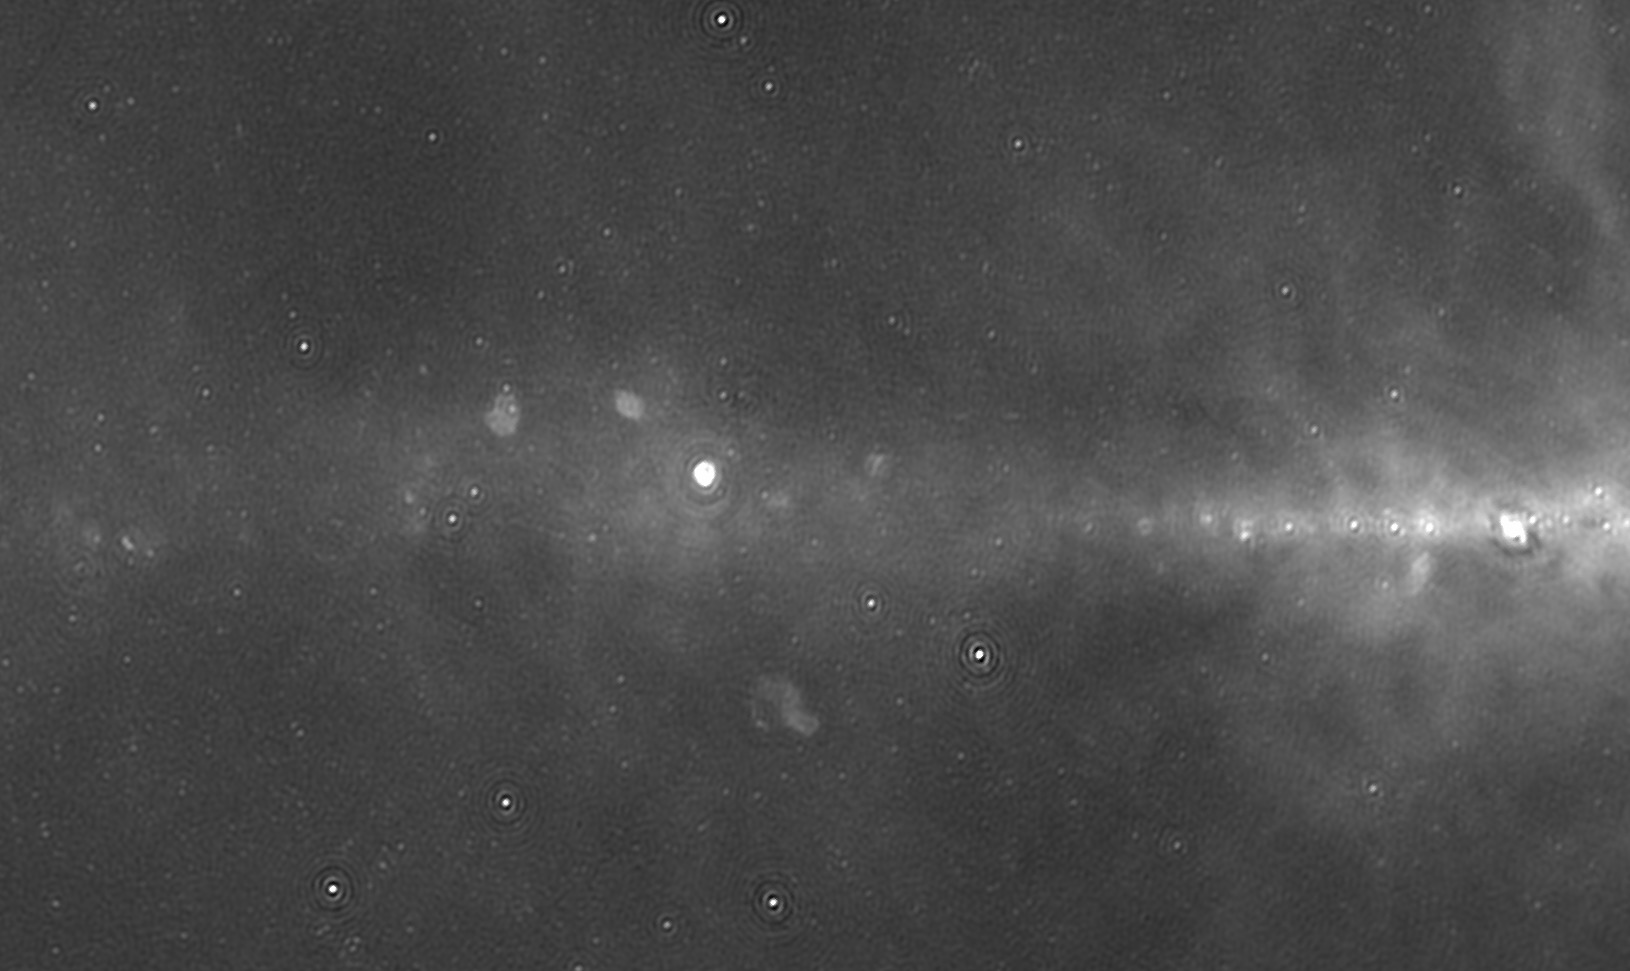
\includegraphics[height=\paperheight]{figures/dirty.jpg}}
    \begin{frame}{Dirty Map}
    \end{frame}

    \usebackgroundtemplate{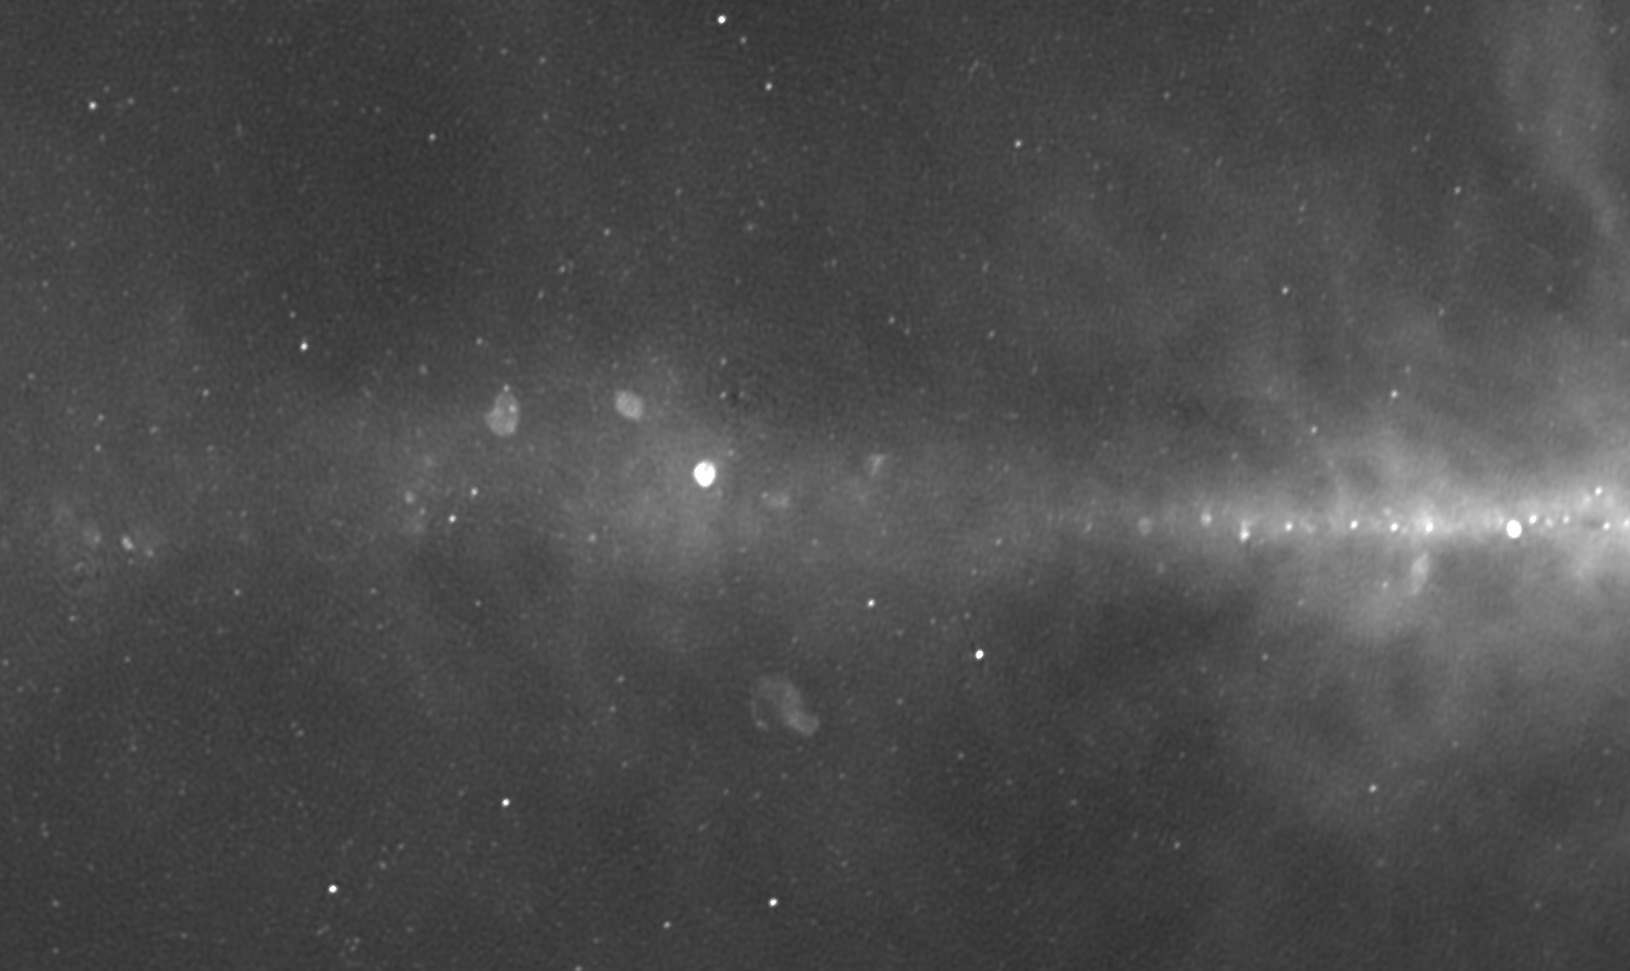
\includegraphics[height=\paperheight]{figures/clean.jpg}}
    \begin{frame}{Clean Map}
    \end{frame}
}

\begin{frame}{Advantages and Disadvantages}
    \textbf{Advantages}
    \begin{itemize}[label=\textbullet]
        \item No gridding step
        \item No mosaicing step
        \item Exact treatment of widefield effects
        \item Optimal foreground filters
    \end{itemize}
    \textbf{Disadvantages}
    \begin{itemize}[label=\textbullet]
        \item Matrix equation is block diagonal, but still large!
        \item 500 GB/frequency channel (!)
        \item Rapid ionospheric changes break assumptions
    \end{itemize}
\end{frame}

\begin{frame}{Eight New Low-Frequency Sky Maps}
    \setlength\tabcolsep{0pt} \Wider[5em]{\begin{tabular}{cccc}
        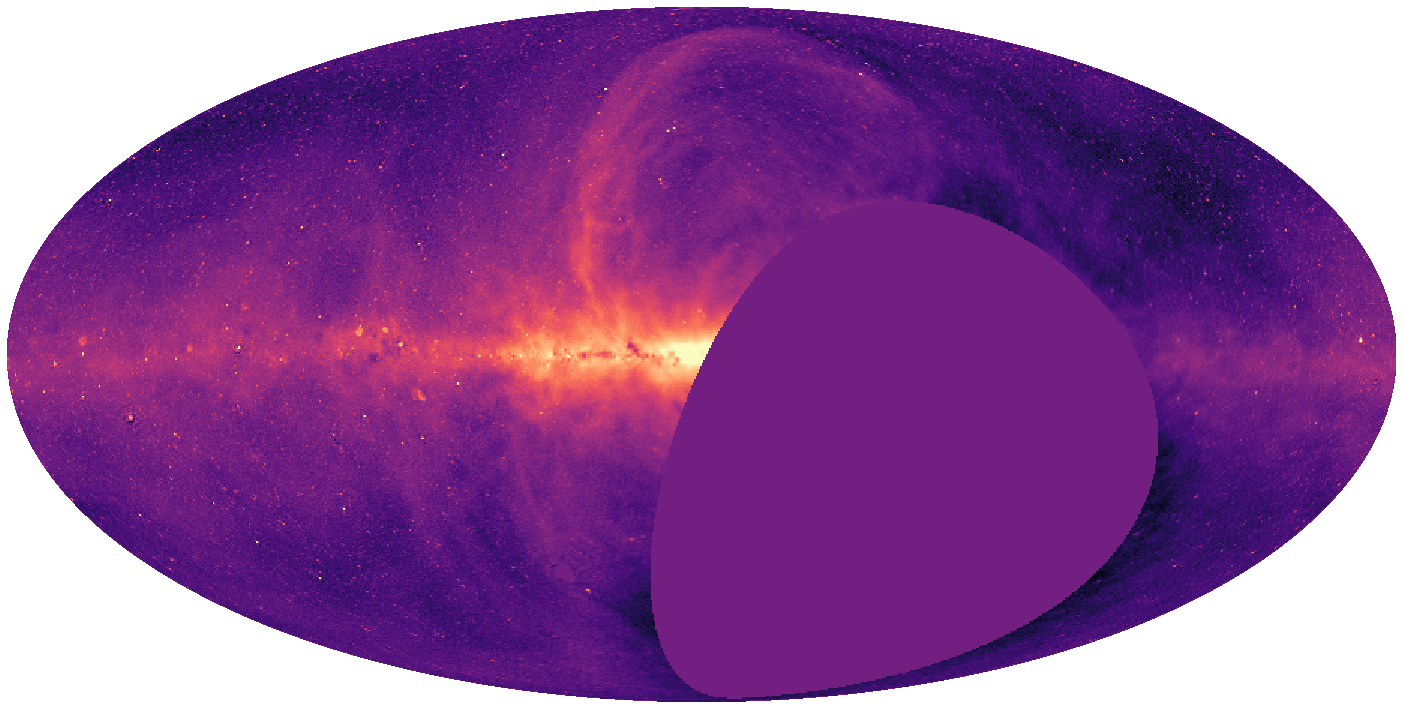
\includegraphics[width=0.25\textwidth]{figures/spw04-notext} &
        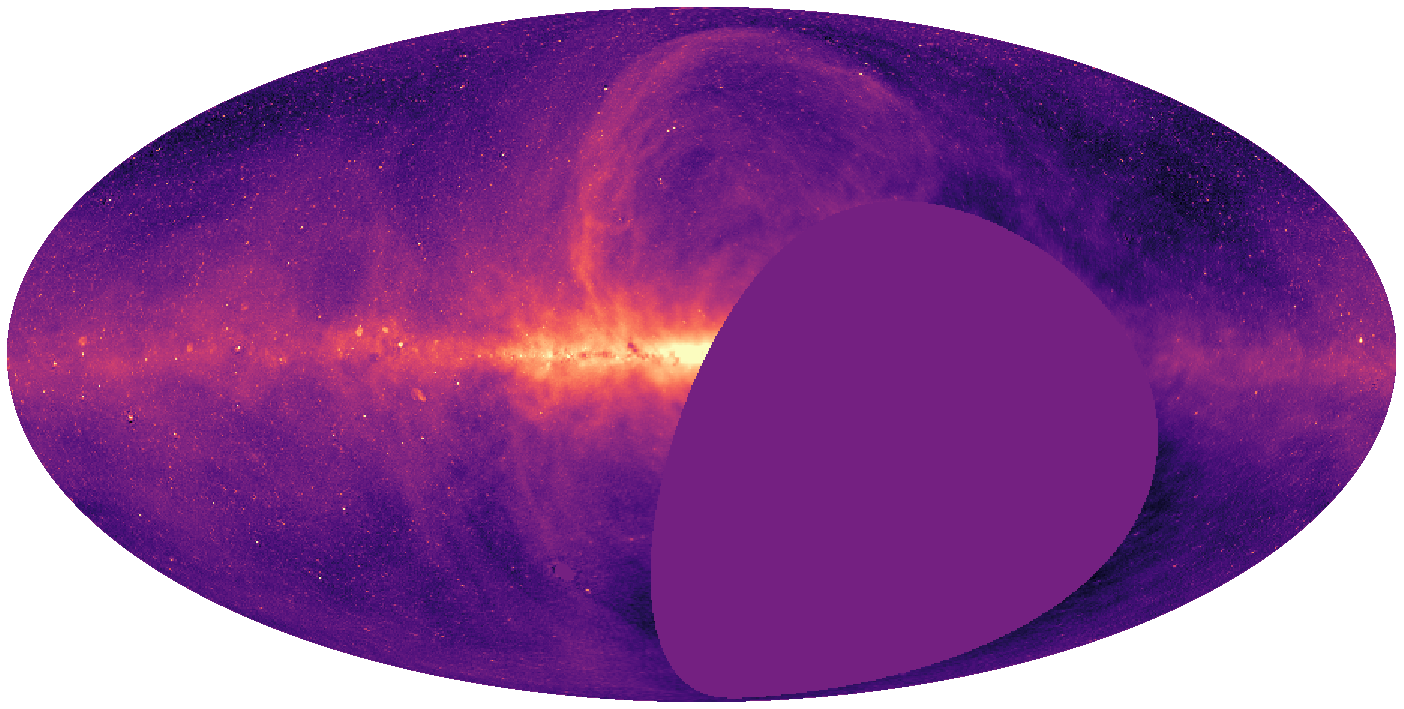
\includegraphics[width=0.25\textwidth]{figures/spw06-notext} &
        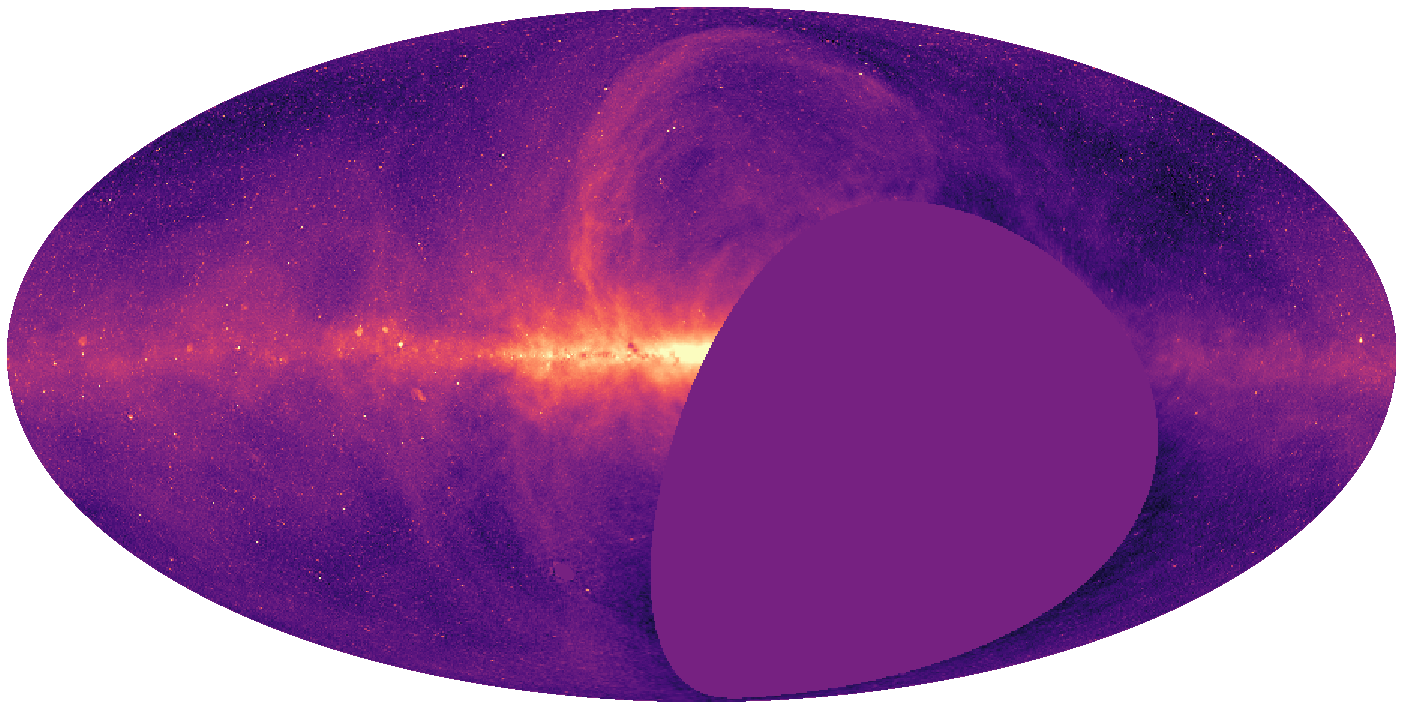
\includegraphics[width=0.25\textwidth]{figures/spw08-notext} &
        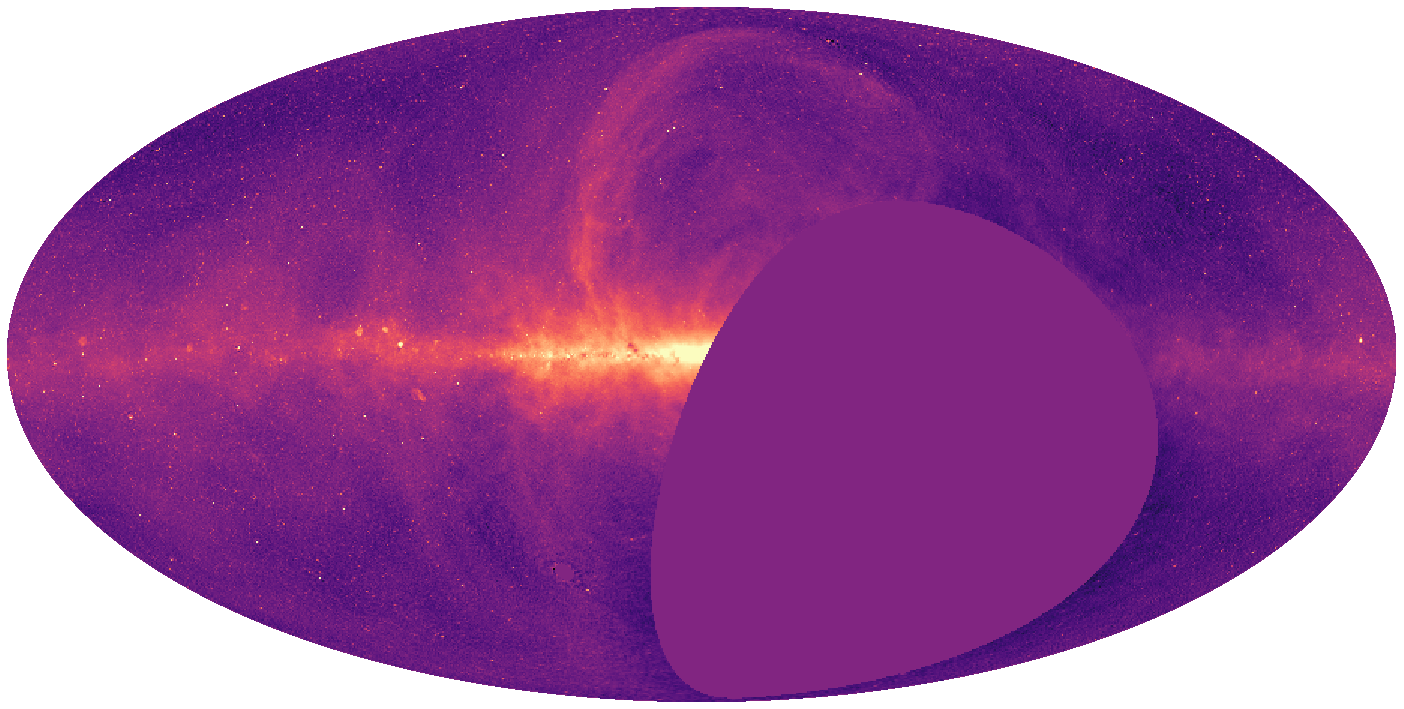
\includegraphics[width=0.25\textwidth]{figures/spw10-notext} \\
        36.528 MHz & 41.760 MHz & 46.992 MHz & 52.224 MHz \\
        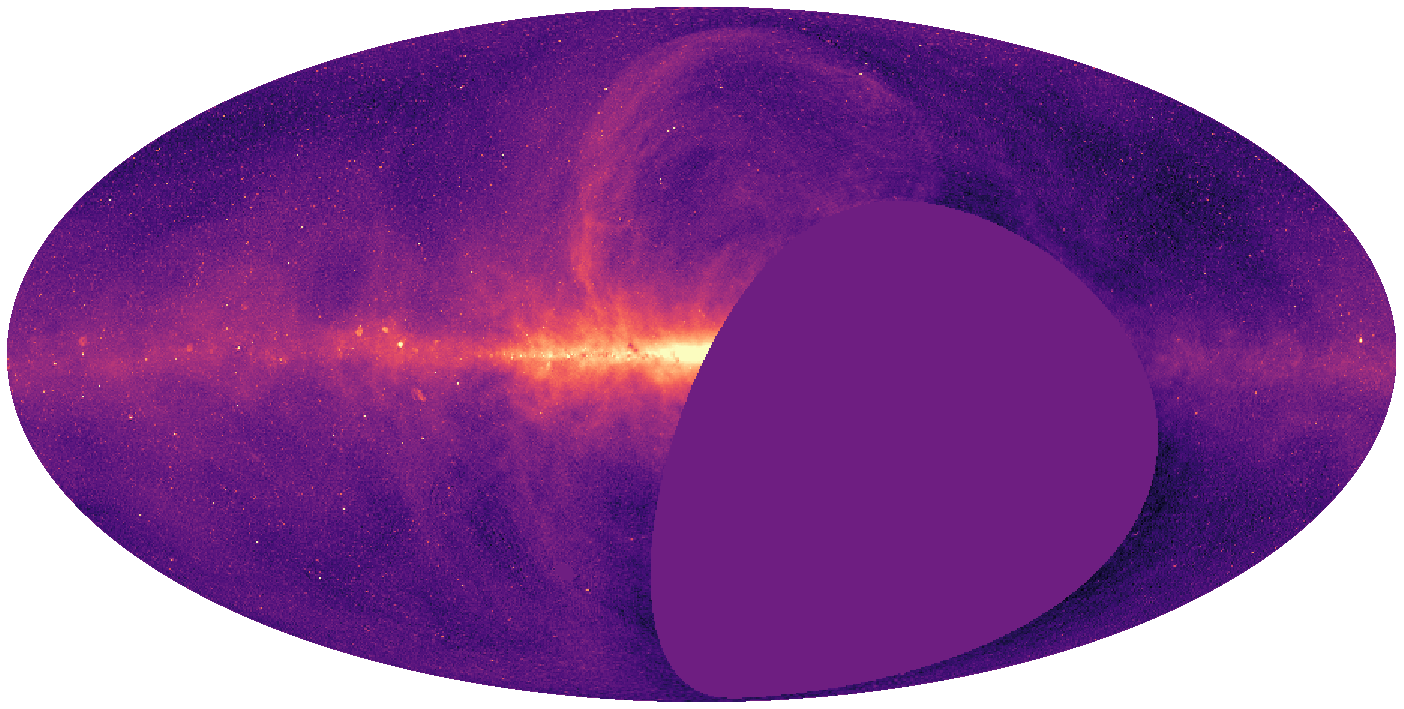
\includegraphics[width=0.25\textwidth]{figures/spw12-notext} &
        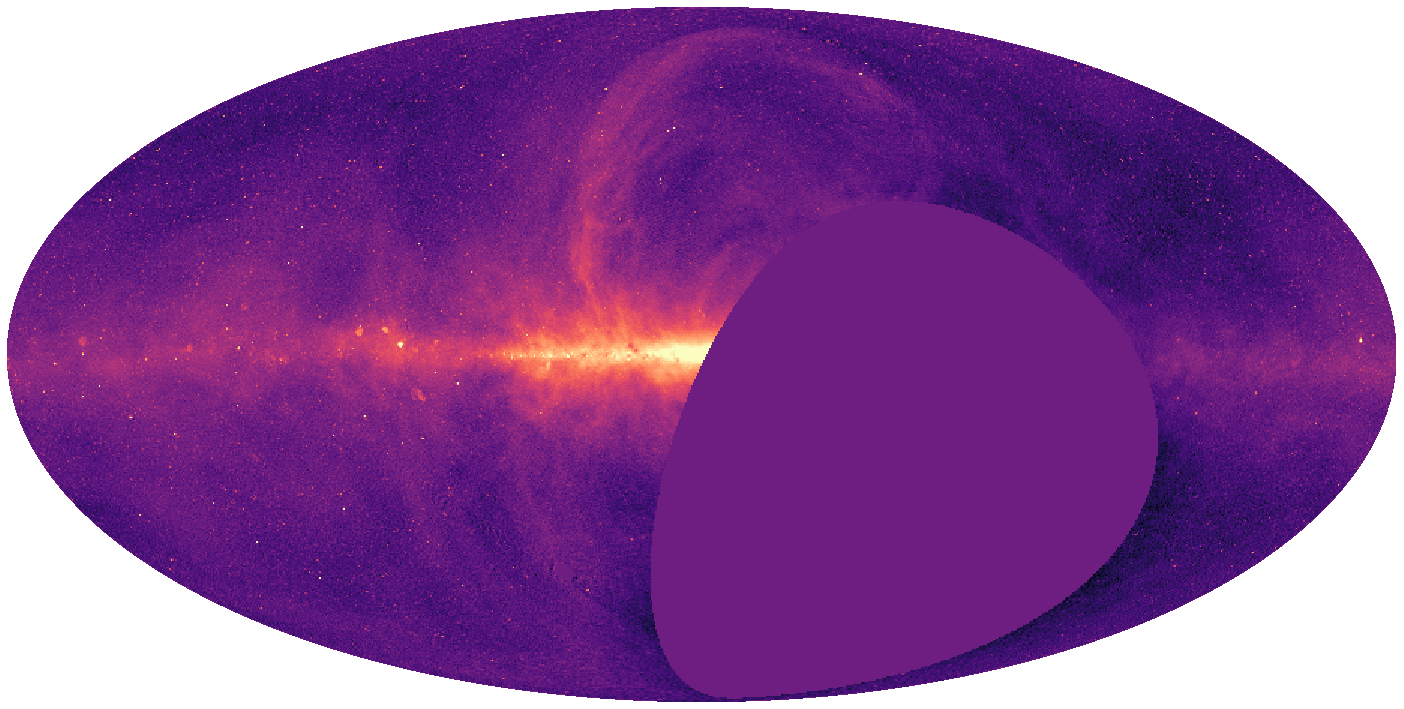
\includegraphics[width=0.25\textwidth]{figures/spw14-notext} &
        \includegraphics[width=0.25\textwidth]{figures/spw16-notext} &
        \includegraphics[width=0.25\textwidth]{figures/spw18-notext} \\
        57.456 MHz & 62.688 MHz & 67.920 MHz & 73.152 MHz \\
    \end{tabular}}
    \begin{center}
        {\tiny Eastwood et al. (2018)}
    \end{center}
    \begin{center}
        {\small \url{https://lambda.gsfc.nasa.gov/product/foreground/ovrolwa_radio_maps_info.cfm}}
    \end{center}
\end{frame}

\begin{frame}{Map Properties}
    \begin{center}
        \begin{tabular}{cccccc}
            \hline
            & \tbf{Frequency} & \tbf{Bandwidth} & \tbf{FWHM} & \multicolumn2c{\tbf{Noise}} \\
            \cline{5-6}
            \tbf{\#} & MHz & kHz & arcmin & K & mJy/beam \\
            \hline
            \rowcolor{red!50!gray} 1 & 36.528 & 24. & 18.5 & 595. & 799. \\
            2 & 41.760 & 24. & 17.2 & 541. & 824. \\
            3 & 46.992 & 24. & 16.3 & 417. & 717. \\
            \rowcolor{green!50!gray} 4 & 52.224 & 24. & 15.6 & 418. & 814. \\
            5 & 57.456 & 24. & 15.4 & 354. & 819. \\
            6 & 62.688 & 24. & 15.3 & 309. & 843. \\
            7 & 67.920 & 24. & 15.3 & 281. & 894. \\
            \rowcolor{blue!50!gray} 8 & 73.152 & 24. & 15.7 & 154. & 598. \\
            \hline
        \end{tabular}
    \end{center}
    \begin{center}
        {\tiny Eastwood et al. (2018)}
    \end{center}
\end{frame}

\begin{frame}{A Three Color Image}
    % Note that all this extra overprint stuff is needed to help make this slide line up with the
    % next one.
    \begin{overprint}
        \onslide<1>
        \Wider[5em]{\includegraphics[width=\textwidth]{figures/ovro-lwa-sky-map-cropped}}
        \begin{center}
            {\tiny Eastwood et al. (2018)} \\
        \end{center}
    \end{overprint}
\end{frame}

\begin{frame}{Comparison with Haslam 408 MHz}
    \begin{overprint}
        \onslide<1>
        \Wider[5em]{\includegraphics[width=\textwidth]{figures/haslam-map}}
        \begin{center}
            {\tiny Haslam et al. (1981, 1982)} \\
        \end{center}
        \onslide<2>
        \Wider[5em]{\includegraphics[width=\textwidth]{figures/ovro-lwa-sky-map-cropped}}
        \begin{center}
            {\tiny Eastwood et al. (2018)} \\
        \end{center}
    \end{overprint}
\end{frame}

\begin{frame}{Comparison with LWA1 (35--80 MHz)}
    \begin{overprint}
        \onslide<1>
        \Wider[5em]{\includegraphics[width=\textwidth]{figures/lwa1}}
        \begin{center}
            {\tiny Dowell et al. (2017)} \\
        \end{center}
        \onslide<2>
        \Wider[5em]{\includegraphics[width=\textwidth]{figures/ovro-lwa-sky-map-cropped}}
        \begin{center}
            {\tiny Eastwood et al. (2018)} \\
        \end{center}
    \end{overprint}
\end{frame}

\begin{frame}{Comparison with Finkbeiner H$\alpha$}
    \begin{overprint}
        \onslide<1>
        \Wider[5em]{\includegraphics[width=\textwidth]{figures/halpha-map}}
        \begin{center}
            {\tiny Finkbeiner et al. (2003)} \\
        \end{center}
        \onslide<2>
        \Wider[5em]{\includegraphics[width=\textwidth]{figures/ovro-lwa-sky-map-cropped}}
        \begin{center}
            {\tiny Eastwood et al. (2018)} \\
        \end{center}
    \end{overprint}
\end{frame}

{
    \usebackgroundtemplate{\includegraphics[height=\paperheight]{figures/before-improved-resolution}}
    \begin{frame}[b]{Higher Resolution, Higher Sensitivity}
        \begin{center}
            {\tiny Eastwood et al. (2018)} \\
        \end{center}
    \end{frame}

    \usebackgroundtemplate{\includegraphics[height=\paperheight]{figures/after-improved-resolution}}
    \begin{frame}[b]{Higher Resolution, Higher Sensitivity}
        \begin{center}
            {\tiny Eastwood et al. (in prep.)} \\
        \end{center}
    \end{frame}
}

{
    \usebackgroundtemplate{\includegraphics[height=\paperheight]{figures/title-slide.jpg}}
    \begin{frame}[t]{Summary}
        \transparent{0.5}
        \colorbox{black}{
            \transparent{1.0}
            \begin{minipage}{\textwidth}
                \begin{itemize}[label=\textbullet]
                    \item Foreground maps are going to be extremely important for 21-cm cosmology
                        experiments going forward.
                    \item Creating high-fidelity foreground maps is also challenging.
                    \item These maps are publicly available online.
                \end{itemize}
                \begin{center}
                    {\small \url{https://lambda.gsfc.nasa.gov/product/foreground/ovrolwa_radio_maps_info.cfm}}
                \end{center}
            \end{minipage}
        }
    \end{frame}
}

%%%%%%%%%%%%%%%%%%%%%%%%%%%%%%%%%%%%%%%%%%%%%%%%%%%%%%%%%%%%%%%%%%%%%%%%%%%%%%%%%%%%%%%%%%%%%%%%%%%%

\section{IV. 21\,cm Power Spectrum}

{
    \usebackgroundtemplate{\includegraphics[height=\paperheight]{figures/waves4}}
    \begin{frame}[t]

        {\large \bfseries IV. Upper Limits on the 21\,cm Power Spectrum ($\b{z>18}$)}
    \end{frame}
}

\begin{frame}{The 3D Spatial Power Spectrum}
    \begin{center}
        \includegraphics[height=0.5\textheight]{figures/cube}
    \end{center}
    Fourier transform and square the brightness temperature in the cosmological cube.
\end{frame}

\begin{frame}{The Foreground Wedge}
    \only<1>{
        \begin{center}
            \includegraphics[height=0.6\textheight]{figures/window}
        \end{center}
    }
    \only<2>{
        \begin{center}
            \includegraphics[height=0.7\textheight]{figures/paper-fringes}
        \end{center}
        \[k_\perp \sim \text{``baseline length''}\]
    }
    \only<3>{
        \begin{block}{XF Correlator}
            \begin{enumerate}
                \item[1.] Cross-correlate voltages at series of time lags (``delays'')
                \item[2.] Fourier transform to obtain frequency spectrum
            \end{enumerate}
        \end{block}

        The Fourier transform along the line of sight undoes the correlator F-stage:

        \[k_\parallel \sim \text{``delay''}\]
    }
    \only<4>{
        \begin{center}
            \includegraphics[height=0.6\textheight]{figures/window}
        \end{center}
    }
\end{frame}

\begin{frame}{Problems with the Foreground Wedge}
    \begin{itemize}[label=\textbullet]
        \item \textbf{Assumes} foreground emission is ``smooth enough''
        \item \textbf{Does not} use any information about the angular structure of the
            foreground emission
        \item \textbf{Does not} use any information about the cosmological emission
        \item \textbf{Does not} account for wide-field effects\\
            {\tiny Thyagarajan et al. 2015}
    \end{itemize}
\end{frame}

\begin{frame}{Covariance Matrices}
    Key advantage of $m$-mode analysis: Full covariance matrices
    \Large
    \[
        \langle \b v \b v^* \rangle =
            \b C = \b C_{\textrm{21}} + \b C_{\textrm{fg}} + \b C_{\textrm{noise}}
    \]
    \normalsize
    Typical size without $m$-mode analysis:
    \Large
    \begin{dmath*}
        (N_{\textrm{baselines}} \times N_{\textrm{frequencies}} \times N_{\textrm{times}})^2
            \times 128\,\textrm{bits} \sim 65\,\textrm{EB}
    \end{dmath*}
    \normalsize
    Typical size with $m$-mode analysis (per matrix block):
    \Large
    \begin{dmath*}
        (l_{\textrm{max}} \times N_{\textrm{frequencies}})^2
            \times 128\,\textrm{bits} \sim 137\,\textrm{MB}
    \end{dmath*}
    \normalsize
\end{frame}

\begin{frame}{The Noise Covariance}
    \only<1>{
        \Large
        \[
            \langle \b v \b v^* \rangle =
                \b C = \b C_{\textrm{21}} + \b C_{\textrm{fg}} + \boxed{\b C_{\textrm{noise}}}
        \]
        \vskip10pt
        \normalsize
        \begin{itemize}[label=\textbullet]
            \item Typically diagonal {\tiny (although see Kulkarni 1989)}
            \item Characterized by the system temperature $T_{\textrm{sys}}$
            \item Measured from variance of visibilities after differencing
            \item Expect sky noise dominated with contribution from receiver
        \end{itemize}
    }
    \only<2>{
        \begin{center}
            \includegraphics[height=0.75\textheight]{figures/system-temperature/system-temperature}
        \end{center}
    }
\end{frame}

\begin{frame}{The Foreground Covariance}
    \only<1>{
        \Large
        \[
            \langle \b v \b v^* \rangle =
                \b C = \b C_{\textrm{21}} + \boxed{\b C_{\textrm{fg}}} + \b C_{\textrm{noise}}
        \]
        \normalsize
        \[
            \Big\langle a_{lm}(\nu)\,a_{l^\prime m^\prime}(\nu + \Delta\nu) \Big\rangle =
                C_l(\nu,\,\Delta\nu)\,\delta_{ll^\prime}\,\delta_{mm^\prime}
        \]
        \vskip10pt
        \begin{itemize}[label=\textbullet]
            \item Dominated by the galactic synchrotron emission
            \item Contribution of point sources increases on small angular scales
            \item Measured $C_l(\nu, 0)$ with an optimal quadratic estimator
        \end{itemize}
    }
    \only<2>{
        \begin{center}
            \includegraphics[height=0.75\textheight]{figures/foreground-covariance/foreground-covariance-06}
        \end{center}
    }
\end{frame}

\begin{frame}{The 21\,cm Signal Covariance}
    \only<1>{
        \Large
        \[
            \langle \b v \b v^* \rangle =
                \b C = \boxed{\b C_{\textrm{21}}} + \b C_{\textrm{fg}} + \b C_{\textrm{noise}}
        \]
        \normalsize
        \[
            P_{\textrm{model}}(k) = \frac{2\pi^2}{k^3}\,\textrm{min}\left[
                40\left(\frac{k}{0.03\,\textrm{Mpc}^{-1}}\right)^2,\,400
            \right]\,\textrm{mK}^2
        \]
        \vskip10pt
        \begin{itemize}[label=\textbullet]
            \item Simple fiducial model {\tiny (Fialkov et al. 2014)}
            \item If EDGES detection is true, power spectrum amplitude reasonably expected to be 50
                times brighter\\
                {\tiny (Bowman et al. 2018, Barkana 2018)}
        \end{itemize}
    }
    \only<2>{
        \begin{center}
            \includegraphics[height=0.75\textheight]{figures/sky-covariance/sky-covariance}
        \end{center}
    }
\end{frame}

\begin{frame}{The Karhunen--Lo\`{e}ve Transform}
    \begin{overprint}
        \onslide<1>
        \begin{center}
            \Wider[4em]{\includegraphics[width=\textwidth]{figures/foreground-filtering-illustration/foreground-filtering-illustration-1}}
        \end{center}
        \onslide<2>
        \begin{center}
            \Wider[4em]{\includegraphics[width=\textwidth]{figures/foreground-filtering-illustration/foreground-filtering-illustration-2}}
        \end{center}
        \onslide<3>
        \begin{center}
            \Wider[4em]{\includegraphics[width=\textwidth]{figures/foreground-filtering-illustration/foreground-filtering-illustration-3}}
        \end{center}
    \end{overprint}
\end{frame}

\begin{frame}{Filtered Image}
    \begin{overprint}
        \onslide<1>
        \begin{center}
            \Wider[3em]{\includegraphics[width=\textwidth]{figures/sky-maps/filtered-sky-map-colorbar}}
        \end{center}
        \onslide<2>
        \begin{center}
            \Wider[3em]{\includegraphics[width=\textwidth]{figures/sky-maps/filtered-sky-map-colorbar-2}}
        \end{center}
    \end{overprint}
\end{frame}

\begin{frame}{Power Spectrum Estimate}
    \begin{overprint}
        \onslide<1>
        \begin{center}
            \includegraphics[height=0.75\textheight]{figures/spherical-power-spectra/spherical-power-spectrum-filter-strength-1.pdf}
        \end{center}
        \onslide<2>
        \begin{center}
            \includegraphics[height=0.75\textheight]{figures/spherical-power-spectra/spherical-power-spectrum-filter-strength-2.pdf}
        \end{center}
        \onslide<3>
        \begin{center}
            \includegraphics[height=0.75\textheight]{figures/spherical-power-spectra/spherical-power-spectrum-filter-strength-3.pdf}
        \end{center}
    \end{overprint}
\end{frame}

\begin{frame}{Power Spectrum Limits}
    \begin{center}
        \includegraphics[height=0.75\textheight]{figures/power-spectrum-upper-limits/power-spectrum-upper-limits}
    \end{center}
\end{frame}

\begin{frame}{Bandpass Errors}
    \begin{center}
        \Wider[3em]{\includegraphics[width=\textwidth]{figures/sky-maps/channel-difference-sky-map-colorbar}}
    \end{center}
\end{frame}

\begin{frame}{Systematic Limitations}
    \begin{overprint}
        \onslide<1>
        \begin{center}
            \includegraphics[height=0.75\textheight]{figures/spherical-power-spectra/spherical-power-spectrum-gain-errors-1.pdf}
        \end{center}
        \onslide<2>
        \begin{center}
            \includegraphics[height=0.75\textheight]{figures/spherical-power-spectra/spherical-power-spectrum-gain-errors-2.pdf}
        \end{center}
        \onslide<3>
        \begin{center}
            \includegraphics[height=0.75\textheight]{figures/spherical-power-spectra/spherical-power-spectrum-gain-errors-3.pdf}
        \end{center}
        \onslide<4>
        \begin{center}
            \includegraphics[height=0.75\textheight]{figures/spherical-power-spectra/spherical-power-spectrum-bandpass-errors.pdf}
        \end{center}
    \end{overprint}
\end{frame}

\begin{frame}{Conclusions}
    \begin{itemize}[label=\textbullet]
        \item
            First measured upper limit of the 21\,cm power spectrum at $z > 18$
        \item
            Lowest upper limit $\Delta_{21}^2 \lesssim (10^4\,\textrm{mK})^2$
        \item
            The double KL transform foreground filter is effective if gain errors $<0.1\%$ and
            bandpass errors $<0.01\%$
        \item
            Current upper limits from the OVRO-LWA are consistent with $\sim 1\%$ errors in the
            bandpass
    \end{itemize}
\end{frame}

\section{Summary}

\begin{frame}{Summary}

    {\Large \bfseries This Thesis}
    \vskip8pt
    \hrule
    \vskip8pt
    \begin{enumerate}
        \item[I.] Introduction to 21\,cm Cosmology
        \item[II.] Commissioning the OVRO-LWA
        \item[III.] New Maps of the Sky at Meter Wavelengths
        \item[IV.] Upper Limits on the 21\,cm Power Spectrum ($z>18$)
    \end{enumerate}
\end{frame}

\begin{frame}{A Three Color Image}
    \Wider[5em]{\includegraphics[width=\textwidth]{figures/ovro-lwa-sky-map-cropped}}
    \begin{center}
        {\tiny Eastwood et al. (2018)} \\
    \end{center}
\end{frame}

\begin{frame}{Power Spectrum Limits}
    \begin{center}
        \includegraphics[height=0.75\textheight]{figures/power-spectrum-upper-limits/power-spectrum-upper-limits}
    \end{center}
\end{frame}

\appendix

\begin{frame}
    \textbf{\huge Backup Slides}
\end{frame}

\begin{frame}{Comparison with Guzm\'{a}n 45 MHz}
    \begin{overprint}
        \onslide<1>
        \Wider[5em]{\includegraphics[width=\textwidth]{figures/ovro-lwa-sky-map-cropped}}
        \begin{center}
            {\tiny Eastwood et al. (2018)} \\
        \end{center}
        \onslide<2>
        \Wider[5em]{\includegraphics[width=\textwidth]{figures/guzman}}
        \begin{center}
            {\tiny Guzm\'{a}n et al. (2011)} \\
        \end{center}
    \end{overprint}
\end{frame}

\begin{frame}{Comparison with DRAO 22 MHz}
    \begin{overprint}
        \onslide<1>
        \Wider[5em]{\includegraphics[width=\textwidth]{figures/ovro-lwa-sky-map-cropped}}
        \begin{center}
            {\tiny Eastwood et al. (2018)} \\
        \end{center}
        \onslide<2>
        \Wider[5em]{\includegraphics[width=\textwidth]{figures/drao}}
        \begin{center}
            {\tiny Roger et al. (1999)} \\
        \end{center}
    \end{overprint}
\end{frame}

\begin{frame}{Even--Odd Jackknife}
    \begin{center}
        \Wider[3em]{\includegraphics[width=\textwidth]{figures/sky-maps/even-odd-sky-map-colorbar}}
    \end{center}
\end{frame}

\begin{frame}{Day--Night Jackknife}
\end{frame}

\begin{frame}{Filtering Illustration}
    \begin{center}
        \Wider[3em]{\includegraphics[width=\textwidth]{figures/foreground-filtering-schematic/foreground-filtering-schematic}}
    \end{center}
\end{frame}

\end{document}

